%%% LaTeX Template
%%% This template is made for project reports
%%%	You may adjust it to your own needs/purposes
%%%
%%% Copyright: http://www.howtotex.com/
%%% Date: March 2011

%%% Preamble
\documentclass[10pt]{report}	% Article class of KOMA-script with 11pt font and a4 format

\usepackage[T1]{fontenc}
\usepackage{color}
\usepackage{framed}
\usepackage{textcomp}
\usepackage{listings}
\usepackage{hyperref}
\usepackage[page]{appendix}
\usepackage{graphicx}
\usepackage{verbatim}
\usepackage{amsmath}
\usepackage{xspace}
\usepackage[tt]{titlepic}

\usepackage{sstmacro}

\usepackage[textwidth=7.5in]{geometry}

\definecolor{shadecolor}{rgb}{1,0.8,0.3}
\definecolor{dkgreen}{rgb}{0,0.6,0}
\definecolor{purple}{rgb}{1,0,1}

\newcommand{\todo}[1] {\textcolor{red}{-[#1]-}}


\newcommand{\mytilde}{{\raise.17ex\hbox{$\scriptstyle\sim$}}}

\newcommand{\sstmacro}{{SST/\raise.35ex\hbox{macro}}\xspace}
\newcommand{\eg}{\textit{e.g.}}

\newcommand{\aside}[1]{\begin{framed} #1 \end{framed}}

\newcommand{\inlinefile}[1]{{\lstset{basicstyle=\ttfamily,keywordstyle={}}\lstinline$#1$}}
\newcommand{\inlinecode}[1]{{\lstset{basicstyle=\ttfamily,keywordstyle={},showstringspaces=false}\lstinline$#1$}}
\newcommand{\inlineshell}[1]{{\lstset{basicstyle=\ttfamily,keywordstyle={},showstringspaces=false}\lstinline$#1$}}

\newcommand{\startcpp}{\begin{CppCode}}
\newcommand{\stopcpp}{\end{CppCode}}
\newcommand{\startshell}{\begin{ShellCmd}}
\newcommand{\stopshell}{\end{ShellCmd}}
\newcommand{\startvi}{\begin{ViFile}}
\newcommand{\stopvi}{\end{ViFile}}

\newcommand{\tableConfig}{| p{5cm} | p{2cm} | p{3cm} | p{8cm} |}
\newcommand{\openTable}{\begin{tabular}{\tableConfig}}
\newcommand{\paramType}[1]{\newline (#1)}
\hyphenpenalty=10000
\pagestyle{empty}


\title{SST/macro 7.2: User's Manual}
\titlepic{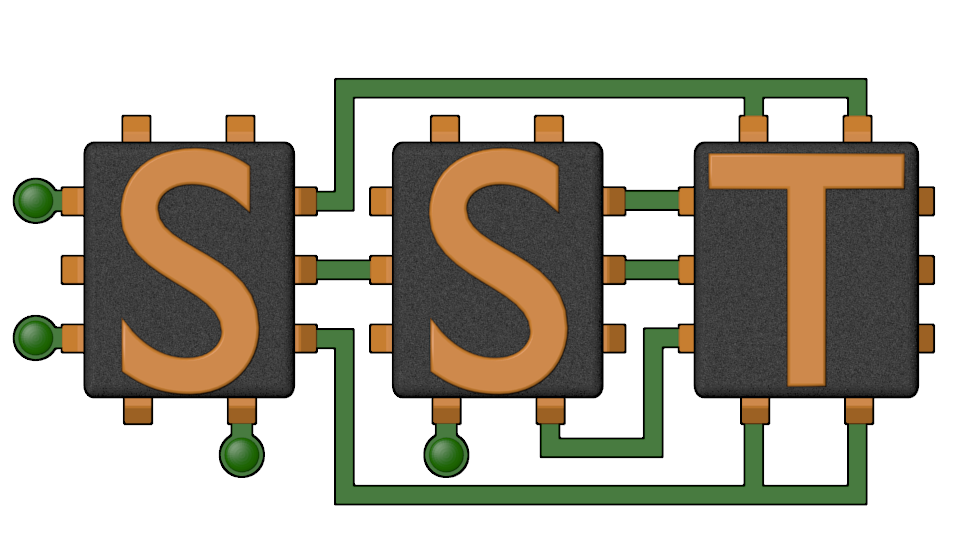
\includegraphics[width=0.3\textwidth]{figures/sstlogo.png}}
\author{Sandia National Labs \\ Livermore, CA}


\setlength{\parindent}{0cm} % Default is 15pt.
\setlength{\parskip}{2mm plus1mm minus1mm}

\begin{document}
\maketitle 


\tableofcontents
%% !TEX root = manual.tex

\chapter{Introduction}
\label{sec:intro}

\section{Overview}
\label{sec:intro:overview}

The \sstmacro software package provides a simulator for large-scale parallel computer architectures. 
It permits the coarse-grained study of distributed-memory applications. 
The simulator is driven from either a trace file or skeleton application. 
The simulator architecture is modular, allowing it to easily be extended with additional network models, 
trace file formats, software services, and processor models.

Simulation can be broadly categorized as either off-line or on-line.
Off-line simulators typically first run a full parallel application on a real machine,
recording certain communication and computation events to a simulation trace.
This event trace can then be replayed post-mortem in the simulator.
Most common are MPI traces which record all MPI events, and
\sstmacro provides the DUMPI utility (\ref{sec:tutorial:dumpi}) for collecting and replaying MPI traces. 
Trace extrapolation can extend the usefulness of off-line simulation by estimating large or untraceable system scales without   
having to collect a trace, but it is limited.

We turn to on-line simulation when the hardware or applications parameters need to change.
On-line simulators instead run real application code, allowing native C/C++ to be compiled directly into the simulator.
\sstmacro intercepts certain function calls, estimating how much time passes rather than actually executing the function.
In MPI programs, for example, calls to MPI\_Send are linked to the simulator instead of passing to the real MPI library.
If desired, \sstmacro can actually be a full MPI \emph{emulator}, delivering messages between ranks and replicating the behavior of a full MPI implementation.

Although \sstmacro supports both on-line and off-line modes, on-line simulation is encouraged because
event traces are much less flexible, containing a fixed sequence of events.
Application inputs and number of nodes cannot be changed. 
Without a flexible control flow, it also cannot simulate dynamic behavior like load balancing or faults.
On-line simulation can explore a much broader problem space since they evolve directly in the simulator.

For large, system-level experiments with thousands of network endpoints, high-accuracy cycle-accurate simulation is not possible,
or at least not convenient.
Simulation requires coarse-grained approximations to be practical.
\sstmacro is therefore designed for specific cost/accuracy tradeoffs.
It should still capture complex cause/effect behavior in applications and hardware, but be efficient enough to simulate at the system-level. 
For speeding up simulator execution, we encourage \textit{skeletonization}, discussed further in Chapter \ref{chap:appsAndSkeletonization}. 
A high-quality skeleton is an application model that reproduces certain characteristics with only limited computation.  
We also encourage uncertainty quantification (UQ) for validating simulator results.
Skeletonization and UQ are the two main elements in the ``canonical'' \sstmacro workflow (Figure \ref{fig:workflow}).

\begin{figure}[t]
  \centering
    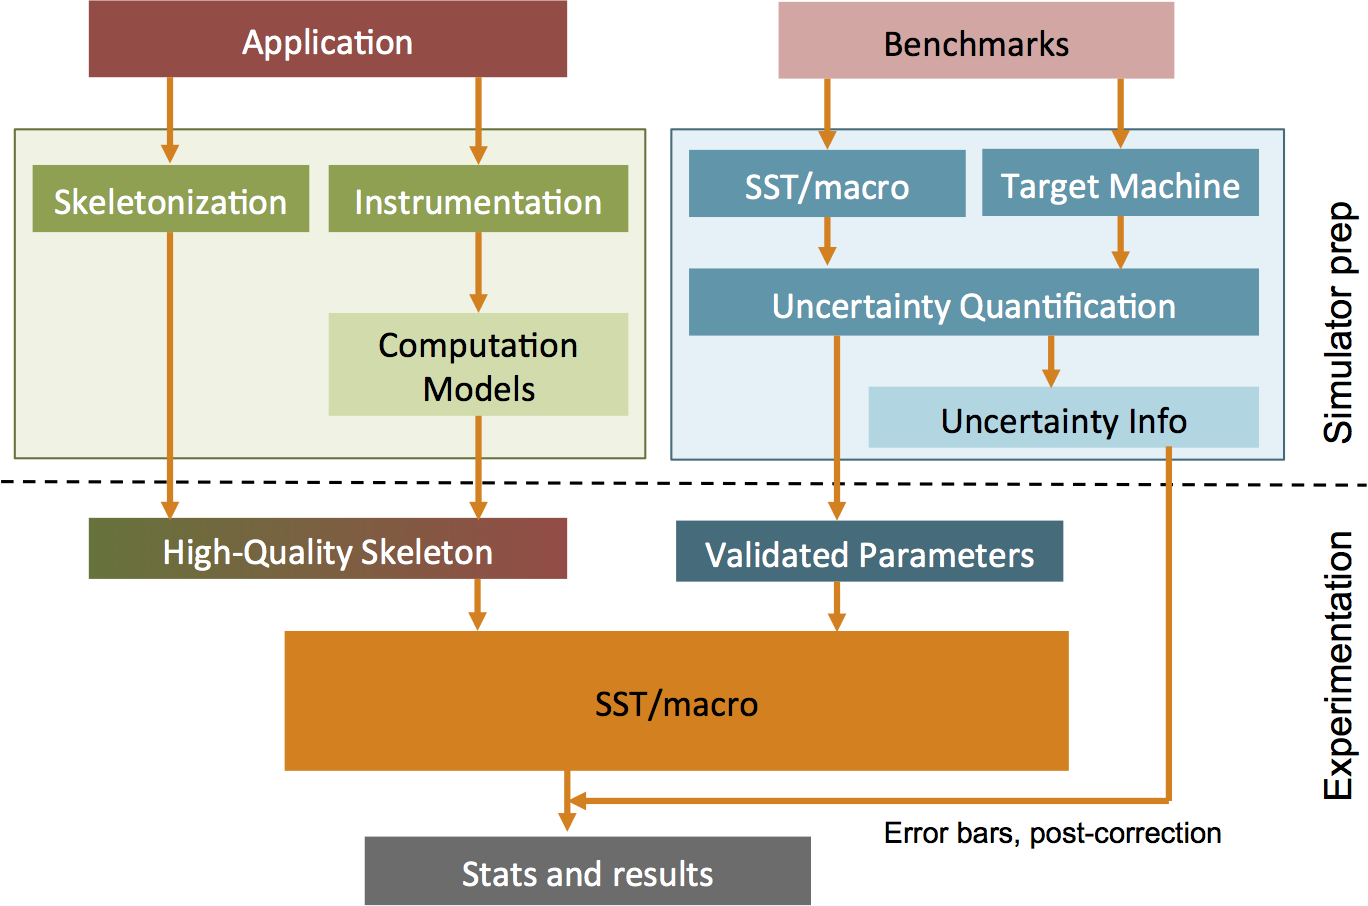
\includegraphics[width=0.99\columnwidth]{figures/workflow.png}
      \caption{SST/macro workflow.}
      \label{fig:workflow}
\end{figure}

Because of its popularity, MPI is one of our main priorities in providing programming model support.  
Some MPI-3 functions and MPI one-sided functions are not implemented.
This will lead to compile errors with an obvious ``not implement'' compiler message.

\section{Preview of Things to Come}
Suppose you have the basic MPI application below that executes a simple send/recv operation.
One could use \inlineshell{mpicc} or \inlineshell{mpic++} to compile and run as an actual MPI program.
This requires spawning all the processes and running them in parallel.
Suppose, however, you wanted to simulate an entire MPI job launch within a single simulator process.
This might prove very useful for debugging since you could just run GDB or Valgrind on a single process.
It might take a while, but for small runs (16 ranks or so) you could debug right on your laptop just as you do for a serial program.

\begin{CppCode}
int size = atoi(argv[1]);
if (rank == 0){
 int partner = 1;
  MPI_Send(buffer, size, MPI_INT, partner, tag, MPI_COMM_WORLD);
} else {
  int partner = 0;
  MPI_Recv(buffer, size, MPI_INT, partner, tag, MPI_COMM_WORLD, MPI_STATUS_IGNORE);
}
MPI_Barrier(MPI_COMM_WORLD);

if (rank == 0){
  printf("Rank 0 finished at t=%8.4f ms\n", MPI_Wtime()*1e3);
}
\end{CppCode}

This is exactly the functionality that SST/macro provides.
Instead of using \inlineshell{mpic++}, you compile the code with \inlineshell{sst++}.
This modifies your code and intercepts MPI calls, running them through the simulator instead of an actual MPI implementation.
Your code will execute and run exactly the same, and your application won't even know the difference.
You now need a parameter file with information like:

\begin{ViFile}
node {
 app1 {
  name = send_recv
  launch_cmd = aprun -n 2
  argv = 20
 }
}
\end{ViFile}
Rather than launching your code using \inlineshell{mpirun} or similar, you put all your command line parameters into a \inlineshell{parameters.ini} file.
The simulator then executes your application exactly as if you had been a real system and run:

\begin{ShellCmd}
shell> aprun -n 2 ./send_recv 20
\end{ShellCmd}
Things get more complicated when you bring skeletonization into play.
The use case above is \emph{emulation}, exactly reproducing MPI functionality.
In \emph{skeletonization} or \emph{simulation}, SST/macro will mimic as closely as possible the original application,
but avoids as much computation and as much memory allocation as possible.
This allows packing in as many simulated (virtual) MPI ranks as possible into your single \inlineshell{sstmac} process.

\section{What To Expect In The User's Manual}
This user's manual is mainly designed for those who wish to perform experiments with \emph{new} applications using \emph{existing} hardware models.
This has been the dominant use case and we therefore classify those doing application experiments as ``users'' and those making new hardware models ``developers.''
Getting applications to run in SST/macro should be very straightforward and requires no knowledge of simulator internal code.
Making new hardware models is much more in depth and requires learning some basics of core simulator code.
Those interested in making new hardware models should consult the developer's manual in the top-level source directory.

%% !TEX root = manual.tex

\chapter{Building and Running SST/macro}
\label{chapter:building}

\section{Build and Installation of \sstmacro}
\label{sec:buildinstall}


\subsection{Downloading}
\label{subsec:build:downloading}

\sstmacro is available at \url{https://github.com/sstsimulator/sst-macro}

\begin{ShellCmd}
shell> git clone https://github.com/sstsimulator/sst-macro.git 
\end{ShellCmd}
or for ssh

\begin{ShellCmd}
shell> git clone ssh://git@github.com/sstsimulator/sst-macro.git 
\end{ShellCmd}

\subsection{Dependencies}
\label{subsec:build:dependencies}
The most critical change is that C++11 is now a strict prerequisite. 
Workarounds had previously existed for older compilers. 
These are no longer supported.
The following are dependencies for \sstmacro.

\begin{itemize}
\item (optional) Git is needed in order to clone the source code repository, but you can also download a tar (Section \ref{subsec:build:downloading}).
\item (Mac) You need the GNU pth library. Downloadable from MacPorts (see Section \ref{subsubsec:pth})
\item Autoconf: 2.68 or later 
\item Automake: 1.11.1 or later 
\item Libtool: 2.4 or later 
\item A C/C++ compiler is required with C++11 support.  gcc >=4.8 and clang >= 3.7 are known to work.
\item (optional) OTF2: 2.0 or later for OTF2 trace replay.
\item (optional) Doxygen and Graphviz are needed to build the documentation.
\item (optional) KCacheGrind or QCacheGrind to display call graphs
\item (optional) Clang development libraries to enable SST source-to-source compiler
\end{itemize}

\subsection{Configuration and Building}
\label{subsec:build:configure}

SST/macro is an SST element library, proving a set of simulation components that run on the main SST core.  
The SST core provides the parallel discrete event simulation manager that manages time synchronization and sending events in serial, MPI parallel, multi-threaded, or MPI + threaded mode.  
The core does not provide any simulation components like node models, interconnect models, MPI trace readers, etc.  
The actual simulation models are contained in the element library.  

The SST core is a standalone executable that dynamically loads shared object files containing the element libraries.  
For many element libraries, a Python input file is created that builds and connects the various simulation components.  
For maximum flexibility, this will become the preferred mode.  
However, SST/macro has historically had a text-file input \inlineshell{parameters.ini} that configures the simulation.  
To preserve that mode for existing users, a wrapper Python script is provided that processes SST/macro input files.  
SST/macro can also be compiled in standalone mode that uses its own simulation core.

The workflow for installing and running on the main SST core is:
\begin{itemize}
\item	Build and install SST core
\item Build and install the SST/macro element library \inlineshell{libmacro.so} 
\item Make sure paths are properly configured for \inlineshell{libmacro.so} to be visible to the SST core (\inlineshell{SST_LIB_PATH})
\item Run the \inlineshell{pysstmac} wrapper Python script that runs SST/macro-specific parameters OR
\item Write a custom Python script 
\end{itemize}

The workflow for installing and running on the standalone SST/macro core (for debugging, not for production):
\begin{itemize}
\item Build and install SST/macro standalone to generate \inlineshell{sstmac} executable
\item Run \inlineshell{sstmac} with \inlineshell{*.ini} parameter files
\end{itemize}

\subsubsection{Build SST core}\label{subsec:buildSSTCore}
The recommended mode for maximum flexibility is to run using the SST core downloadable from \url{http://sst-simulator.org/SSTPages/SSTMainDownloads/}.
Building and installing sets up the discrete event simulation core required for all SST elements.
SST core no longer has Boost dependencies! Directions for building Boost (if desired) are still below in \ref{subsubsec:boost}

\subsubsection{Build SST/macro element library}\label{subsec:buildElementLib}
Once \sstmacro is extracted to a directory, we recommend the following as a baseline configuration, including building outside the source tree:

\begin{ShellCmd}
sst-macro> ./bootstrap.sh
sst-macro> mkdir build
sst-macro> cd build
sst-macro/build> ../configure --prefix=$PATH_TO_INSTALL --with-sst-core=$PATH_TO_SST_CORE CC=$MPICC CXX=$MPICXX
\end{ShellCmd}
\inlinecode{PATH_TO_SST_CORE} should be the prefix install directory used when installing the core.  
The MPI compilers should be the same compilers used for building Boost and SST core.

SST/macro can still be built in standalone mode for a select set of features that have not been fully migrated to the SST core.  
The installation and running are the same for both modes - simply remove the \inlineshell{--with--sst-core} parameter.  
A complete list of options for standalone building can be seen by running \inlineshell{../configure --help}.   Some common options include:

\begin{itemize}
\item --(dis|en)able-graphviz : Enables the collection of simulated call graphs, which can be viewed with graphviz.
Enabled by default. Disable if not using Boost or C++11. Ordered maps can be used as a replacement, but with lower performance.
\item --(dis|en)able-regex : Regular expressions can be used to proofread input files, but this requires either Boost or C++11.
Enabled by default. Disable if not using Boost or C++11.
\item --(dis|en)able-custom-new : Memory is allocated in larger chunks in the simulator, which can speed up large simulations.
\item --(dis|en)able-multithread : This configures for thread-level parallelism for (hopefully) faster simulation
\item --(dis|en)able-otf2: Enable OTF2 trace replay, requires a path to OTF2 installation.
\item --with-clang[=location]: Enable Clang source-to-source tools by pointing to Clang development libraries
\end{itemize}

Once configuration has completed, printing a summary of the things it found, simply type \inlineshell{make}.  

\subsection{Post-Build}
\label{subsec:postbuild}

If the build did not succeed, check \ref{subsec:build:issues} for known issues, or contact \sstmacro support for help (sst-macro-help@sandia.gov).

If the build was successful, it is recommended to run the range of tests to make sure nothing went wrong.  
To do this, and also install \sstmacro  to the install path specified during installation, run the following commands:

\begin{ShellCmd}
sst-macro/build> make check
sst-macro/build> make install
sst-macro/build> make installcheck
\end{ShellCmd}
Make check runs all the tests we use for development, which checks all functionality of the simulator.  
Make installcheck compiles some of the skeletons that come with \sstmacro, linking against the installation.  

\aside{
Important:  Applications and other code linking to \sstmacro use Makefiles that use the sst++/sstcc compiler wrappers
that are installed there for convenience to figure out where headers and libraries are.  Make sure your path is properly configured.
}

\subsection{GNU pth for user-space threading}\label{subsubsec:pth}
By default, Linux usually ships with \inlineshell{ucontext} which enables user-space threading.
Mac OS X does not support \inlineshell{ucontext} and requires an extra library be installed (GNU pth).
GNU pth is easy to download and install from source.
Even easier is MacPorts. 

\begin{ShellCmd}
shell> sudo port install pth
\end{ShellCmd}

MacPorts installed all libraries to \inlineshell{/opt/local}. 
When configuring, simply add \inlineshell{--with-pth=\$PATH_TO_PTH} as an argument.
For MacPorts installation, this means configuring SST/macro with:

\begin{ShellCmd}
../configure --with-pth=/opt/local
\end{ShellCmd}

\subsection{Building Boost (no longer required)}\label{subsubsec:boost}
We recommend two files: \inlineshell{user-config.jam} to configure the Boost compiler flags and a \inlineshell{runme.sh} that bootstraps, compiles, and installs the prerequisite Boost libraries. For GCC, the \inlineshell{user-config.jam} should go in the top-level home directory and the file should contain the line:

\begin{ViFile}
using gcc : : $PATH_TO_MPIC++  : <compileflags>-std=c++1y ;
\end{ViFile}
For Clang on Mac, use:

\begin{ViFile}
using clang : : $PATH_TO_CLANG_MPIC++  : <compileflags>-std=c++1y <linkflags>-stdlib=libc++ 
\end{ViFile}

We recommend Boost 1.59.  Other Boost versions should work as well, but this seems the most stable.  In the top-level Boost directory, make a script \inlineshell{runme.sh} that contains:

\begin{ViFile}
./bootstrap.sh \
  --with-libraries=program_options,serialization,filesystem \
  --with-toolset=gcc

./b2 ---prefix=$INSTALL
./b2 --layout=tagged --prefix=$INSTALL
\end{ViFile}

The toolset can be changed from gcc to clang, as needed.  For maximum safety, Boost should install both ``tagged" versions of libraries and un-tagged versions.  Once Boost is installed with these options, configuration and installation of SST core should be straightforward following documentation in the core library.

\subsection{Known Issues}
\label{subsec:build:issues}


\begin{itemize}
\item Any build or runtime problems should be reported to sst-macro-help@sandia.gov.  We try to respond as quickly as possible.
\item make -j: When doing a parallel compile dependency problems can occur.  
There are a lot of inter-related libraries and files.  
Sometimes the Makefile dependency tracker gets ahead of itself and you will get errors about missing libraries and header files.
If this occurs, restart the compilation.  If the error vanishes, it was a parallel dependency problem.
If the error persists, then it's a real bug.
\item GNU pth: For Mac, make sure to follow directions in \ref{subsubsec:pth} to ensure pth is correctly installed.
\item Ubuntu: The Ubuntu linker performs too much optimization on dynamically linked executables.
Some call it a feature.  I call it a bug.
In the process it throws away symbols it actually needs later. The build system should automatically fix Ubuntu flags.
If still having issues, make sure that '-Wl,--no-as-needed' is given in LDFLAGS.

The problem occurs when the executable depends on libA which depends on libB.
The executable has no direct dependence on any symbols in libB.
Even if you add \inlineshell{-lB} to the \inlineshell{LDFLAGS} or \inlineshell{LDADD} variables,
the linker ignores them and throws the library out.
It takes a dirty hack to force the linkage.
If there are issues, contact the developers at sst-macro-help@sandia.gov and report the problem. 
\end{itemize}

\section{Building DUMPI}
\label{sec:building:dumpi}

By default, DUMPI is configured and built along with SST/macro with support for reading and parsing DUMPI traces, known as libundumpi.  
DUMPI binaries and libraries are also installed along with everything for \sstmacro during make install.   
DUMPI can be used as its own library within the \sstmacro source tree by changing to \inlineshell{sst-macro/sst-dumpi}, 
where you can change its configuration options.  

DUMPI can also be used as stand-alone tool (\eg~for simplicity if you're only tracing). 
To get DUMPI by itself, either copy the \inlineshell{sstmacro/dumpi} directory somewhere else or visit \url{https://github.com/sstsimulator/sst-dumpi} and follow similar instructions for obtaining \sstmacro.

To see a list of configuration options for DUMPI, run \inlineshell{./configure --help}.  
If you're trying to configure DUMPI for trace collection, use \inlineshell{--enable-libdumpi}.
Your build process might look like this (if you're building in a separate directory from the dumpi source tree) :

\begin{ShellCmd}
sst-dumpi/build> ../configure --prefix=/path-to-install --enable-libdumpi
sst-dumpi/build> make
sst-dumpi/build> sudo make install
\end{ShellCmd}

\subsection{Known Issues}
\label{subsubsec:building:dumpi:issues}

\begin{itemize}
\item When compiling on platforms with compiler/linker wrappers, e.g. ftn (Fortran) and CC (C++) compilers 
at NERSC, the libtool configuration can get corrupted.  The linker flags automatically added by the 
wrapper produce bad values for the predeps/postdeps variable in the libtool script in the top 
level source folder.  When this occurs, the (unfortunately) easiest way to fix this is to manually modify
the libtool script.  Search for predeps/postdeps and set the values to empty.
This will clear all the erroneous linker flags.  The compilation/linkage should still work since 
all necessary flags are set by the wrappers. 
\end{itemize}

\section{Building with OTF2 (Beta)}
\label{sec:buildingOtf2}
OTF2 is a general purpose trace format with specialized callbacks for the MPI API. OTF2 traces are generated by programs compiled with Score-P compiler wrappers. SST/macro 7.0 supports OTF2 trace replay when configured with 

\begin{ViFile}
./configure --enable-otf2=<OTF2-root>	
\end{ViFile}
where the OTF2 root is the installation prefix for a valid OTF2 build. OTF2 can be obtained from the Score-P project at {http://www.vi-hps.org/projects/score-p}.
Detailed build and usage instructions can be found on the website.


\section{Building Clang source-to-source support}
\label{sec:buildingClang}

To enable Clang source-to-source support it is not sufficient to have a Clang compiler.  You have to install a special libTooling library for Clang.

\subsection{Building Clang libTooling}
\label{subsec:buildingClanglibTooling}

\subsubsection{The Easy Way: Mac OS X}
\label{subsubsec:libToolingOSX}
Using MacPorts on OS X, it is trivial to obtain a Clang installation that includes libTooling:

\begin{ViFile}
port install clang-devel
\end{ViFile}

MacPorts will place the Clang compilers in \inlineshell{/opt/local/bin}.  Enable the devel version of Clang with:

\begin{ViFile}
port select --set clang mp-clang-devel
\end{ViFile}

The Clang libraries will be placed into \inlineshell{/opt/local/libexec/llvm-devel/lib}, so the appropriate option to the sst-macro configure script is \inlineshell{--with-clang=/opt/local/libexec/llvm-devel}.

\subsubsection{The Hard Way}
\label{subsubsec:libTooling}
For operating systems other than OS X, building Clang support has a few steps (and takes quite a while to build), but is straightforward.
Instead of having an all-in-one tarball, you will have to download 2 different components. You can install more if you want build libc++, but these are not required.
Obtain the following from \url{http://releases.llvm.org/download.html}.

\begin{itemize}
\item LLVM source code
\item Clang source code
\item (optional, not recommended unless needed) libc++ source code
\item (optional, not recommended unless needed) libc++abi source code
\item (optional, not recommended) compiler-rt source code
\item (optional, not recommended) OpenMP source code
\end{itemize}

Setting up the folders can be done automatically using the \inlineshell{setup-clang} script in \inlineshell{bin/tools} folder in sst-macro. Put all of downloaded tarballs in a folder, e.g. \inlineshell{clang-llvm}. Then run \inlineshell{setup-clang} in the directory. 
It will automatically place files where LLVM needs them.
LLVM is the ``driver'' for the entire build. Everything else is a subcomponent. 
The setup script places each tarball in the following subfolders of the main LLVM folder

\begin{itemize}
\item tools/clang
\item projects/compiler-rt
\item projects/libc++
\item projects/libc++abi
\item projects/openmp
\end{itemize}

Only Clang is a strict dependency. Using CMake (assuming you are in a build subdirectory of the LLVM tree), you would run the script below to configure.
You MUST use another Clang compiler to build. If not, then you need to bootstrap (use GCC to build Clang, then use that Clang to build itself).

\begin{ViFile}
cmake ../llvm \
  -DCMAKE_CXX_COMPILER=clang++ \
  -DCMAKE_C_COMPILER=clang \
  -DCMAKE_CXX_FLAGS="-O3" \
  -DCMAKE_C_FLAGS="-O3" \
  -DCMAKE_INSTALL_PREFIX=$install
\end{ViFile}

To build a complete LLVM/Clang (again, not required unless you absolutely need a new libc++), run:

\begin{ViFile}
cmake ../llvm \
  -DCMAKE_CXX_COMPILER=clang++ \
  -DCMAKE_C_COMPILER=clang \
  -DCMAKE_CXX_FLAGS="-O3" \
  -DCMAKE_C_FLAGS="-O3" \
  -DLLVM_ENABLE_LIBCXX=ON \
  -DLLVM_TOOL_COMPILER_RT_BUILD=ON \
  -DLLVM_TOOL_LIBCXXABI_BUILD=ON \
  -DLLVM_TOOL_LIBCXX_BUILD=ON \
  -DCMAKE_INSTALL_PREFIX=$install
\end{ViFile}

On some systems, linking Clang might blow out your memory. If that is the case, you have to set \inlineshell{LD=ld.gold} for the linker.
Run \inlineshell{make install}. The libTooling library will now be available at the \inlineshell{\$install} location.

\subsection{Building SST/macro with Clang}
Now that clang is installled, you only need to add the configure flag \inlineshell{--with-clang} pointing it to the install location from above.
You must use the same Clang compiler to build SST that you used to build libTooling.

\begin{ShellCmd}
../configure CXX=clang++ CC=clang --with-clang=$install
\end{ShellCmd}

Clang source-to-source support will now be built into the \inlineshell{sst++} compiler.

\section{Running an Application}\label{sec:building:running}
\subsection{SST Python Scripts}
\label{subsec:SSTPythonScripts}

Full details on building SST Python scripts can be found at \url{http://sst-simulator.org}.  To preserve the old parameter format in the near-term, SST/macro provides the \inlineshell{pysstmac} script:

\begin{ViFile}
export SST_LIB_PATH=$SST_LIB_PATH:$SSTMAC_PREFIX/lib

options="$@"
$SST_PREFIX/bin/sst $SSTMAC_PREFIX/include/python/default.py --model-options="$options"
\end{ViFile}

The script configures the necessary paths and then launches with a Python script \inlineshell{default.py}.  Interested users can look at the details of the Python file to understand how SST/macro converts parameter files into a Python config graph compatible with SST core.
Assuming the path is configured properly, users can run

\begin{ShellCmd}
>pysstmac -f parameters.ini
\end{ShellCmd}
with a properly formatted parameter file. If running in standalone mode, the command would be similarly (but different).

\begin{ViFile}
from sst.macro import *
setupDeprecated()
\end{ViFile}

\begin{ShellCmd}
>sstmac -f parameters.ini
\end{ShellCmd}
since there is no Python setup involved.

\subsection{Building Skeleton Applications}
\label{sec:tutorial:runapp}

To demonstrate how an external skeleton application is run in \sstmacro, we'll use a very simple send-recv program located in \inlineshell{skeletons/sendrecv}.
We will take a closer look at the actual code in Section \ref{sec:tutorial:basicmpi}.
After \sstmacro has been installed and your PATH variable set correctly, for standalone core users can run:

\begin{ShellCmd}
sst-macro> cd skeletons/sendrecv
sst-macro/skeletons/sendrecv> make
sst-macro/skeleton/sendrecv> ./runsstmac -f parameters.ini
\end{ShellCmd}

You should see some output that tells you 1) the estimated total (simulated) runtime of the simulation, and 
2) the wall-time that it took for the simulation to run.  
Both of these numbers should be small since it's a trivial program. 

This is how simulations generally work in \sstmacro: you build skeleton code and link it with the simulator to produce a binary.  
Then you run that binary and pass it a parameter file which describes the machine model to use.  For running on the main SST core, a few extra flags are required.  Rather than generating a standalone executable, the compiler wrapper generates a shared library. Users can always write their own Python scripts, which will be required for more advanced usage. However, users can also just use the \inlineshell{pysstmac} script.

\begin{ShellCmd}
>sst-macro/skeletons/sendrecv> pysstmac librunsstmac.so -f parameters.ini
\end{ShellCmd}
Any extra shared libraries can be given as the first few parameters and these will automatically be imported.

\subsection{Makefiles}
\label{subsec:tutorial:makefiles}

We recommend structuring the Makefile for your project like the one seen in \inlineshell{skeletons/sendrecv/Makefile} :

\begin{ViFile}
TARGET := runsstmac
SRC := $(shell ls *.c) 

CXX :=      $(PATH_TO_SST)/bin/sst++
CC :=        $(PATH_TO_SST)/bin/sstcc
CXXFLAGS := ...
CPPFLAGS := ...
LIBDIR :=  ...
PREFIX :=   ...
LDFLAGS :=  -Wl,-rpath,$(PREFIX)/lib
...
\end{ViFile}
The SST compiler wrappers \inlineshell{sst++} and \inlineshell{sstcc} automagically configure and map the code for simulation. 

\subsection{Command-line arguments}
\label{subsec:tutorial:cmdline}

There are only a few basic command-line arguments you'll ever need to use with \sstmacro, listed below

\begin{itemize}
\item -h/--help: Print some typical help info
\item -f [parameter file]: The parameter file to use for the simulation.  
This can be relative to the current directory, an absolute path, or the name of a pre-set file that is in sstmacro/configurations 
(which installs to /path-to-install/include/configurations, and gets searched along with current directory). 
\item --dumpi: If you are in a folder with all the DUMPI traces, you can invoke the main \inlinecode{sstmac} executable with this option.  This replays the trace in a special debug mode for quickly validating the correctness of a trace.
\item -d [debug flags]: A list of debug flags to activate as a comma-separated list (no spaces) - see Section \ref{sec:dbgoutput}
\item -p [parameter]=[value]: Setting a parameter value (overrides what is in the parameter file)
\item -t [value]: Stop the simulation at simulated time [value]
\item -c: If multithreaded, give a comma-separated list (no spaces) of the core affinities to use - see Section \ref{subsec:parallelopt}
\end{itemize}

\section{Parallel Simulations in Standalone Mode}
\label{sec:PDES}

\sstmacro supports running parallel discrete event simulation (PDES) in distributed memory (MPI), threaded shared memory (pthreads) and hybrid (MPI+pthreads) modes.  Running these in standalone mode will be discouraged as parallel simulations should use the unified SST core. However, near-term, hybrid modes and other optimizations are not fully supported in the unified SST core. They standalone core may still be required for certain cases.

\subsection{Distributed Memory Parallel}
\label{subsec:mpiparallel}
Configure will automatically check for MPI.
Your configure should look something like:

\begin{ShellCmd}
sst-macro/build> ../configure CXX=mpicxx CC=mpicc ...
\end{ShellCmd}
With the above options, you can just compile and go.
\sstmacro is run exactly like the serial version, but is spawned like any other MPI parallel program.
Use your favorite MPI launcher to run, e.g. for OpenMPI

\begin{ShellCmd}
mysim> mpirun -n 4 sstmac -f parameters.ini
\end{ShellCmd}
or for MPICH

\begin{ShellCmd}
mysim> mpiexec -n 4 sstmac -f parameters.ini
\end{ShellCmd}

Even if you compile for MPI parallelism, the code can still be run in serial with the same configuration options.
\sstmacro will notice the total number of ranks is 1 and ignore any parallel options.
When launched with multiple MPI ranks, \sstmacro will automatically figure out how many partitions (MPI processes) 
you are using, partition the network topology into contiguous blocks, and start running in parallel.   

\subsection{Shared Memory Parallel}
\label{subsec:parallelopt}
In order to run shared memory parallel, you must configure the simulator with the \inlineshell{--enable-multithread} flag.
Partitioning for threads is currently always done using block partitioning and there is no need to set an input parameter.
Including the integer parameter \inlineshell{sst_nthread} specifies the number of threads to be used (per rank in MPI+pthreads mode) in the simulation.
The following configuration options may provide better threaded performance.
\begin{itemize}
\item\inlineshell{--enable-spinlock} replaces pthread mutexes with spinlocks.  Higher performance and recommended when supported.
\item\inlineshell{--enable-cpu-affinity} causes \sstmacro to pin threads to specific cpu cores.  When enabled, \sstmacro will require the
\inlineshell{cpu_affinity} parameter, which is a comma separated list of cpu affinities for each MPI task on a node.  \sstmacro will sequentially
pin each thread spawned by a task to the next next higher core number.  For example, with two MPI tasks per node and four threads per MPI task,
\inlineshell{cpu_affinity = 0,4} will result in MPI tasks pinned to cores 0 and 4, with pthreads pinned to cores 1-3 and 5-7.
For a threaded only simulation \inlineshell{cpu_affinity = 4} would pin the main process to core 4 and any threads to cores 5 and up.
The affinities can also be specified on the command line using the \inlineshell{-c} option.
Job launchers may in some cases provide duplicate functionality and either method can be used.
\end{itemize}

\subsection{Warnings for Parallel Simulation}
\label{subsec:parallelwarn}
\begin{itemize}
\item Watch your \inlineshell{LD_LIBRARY_PATH} if you have multiple different builds. If your paths get scrambled and the wrong libraries are being read, you will get bizarre, inscrutable errors.
\item If the number of simulated processes specified by e.g. \inlinefile{aprun -n 100} does not match the number of nodes in the topology (i.e. you are not space-filling the whole simulated machine), parallel performance will suffer. \sstmacro partitions nodes, not MPI ranks.
\end{itemize}

\aside{
Parallel simulation speedups are likely to be modest for small runs.
Speeds are best with serious congestion or heavy interconnect traffic.
Weak scaling is usually achievable with 100-500 simulated MPI ranks per logical process.
Even without speedup, parallel simulation can certainly be useful in overcoming memory constraints, expanding the maximum memory footprint. 
}

\section{Debug Output}
\label{sec:dbgoutput}
\sstmacro defines a set of debug flags that can be specified in the parameter file to control debug output printed by the simulator.
To list the set of all valid flags with documentation, the user can run

\begin{ShellCmd}
bin> ./sstmac --debug-flags
\end{ShellCmd}

which will output something like

\begin{ViFile}
    mpi
        print all the basic operations that occur on each rank - only API calls are
        logged, not any implementation details
    mpi_check
        validation flag that performs various sanity checks to ensure MPI application
        runs and terminates cleanly
    mpi_collective
        print information about MPI collective calls as well as implementation details
    mpi_pt2pt
        print information about MPI point-to-point calls as well as implementation
        details
     ....
\end{ViFile}
The most important flag for validating simulations is the \inlineshell{mpi_check} flag,
which causes special sanity checks and a final validation check to ensure the simulation has finished cleanly.
Some of the debug flags can generate information overload and will only be useful to a serious developer, rather than a user.

To turn on debug output, add the following to the input file

\begin{ViFile}
debug = mpi  mpi_check
\end{ViFile}
listing all flags you want separated by spaces.
Note: this is a major shift from the previous (and really tedious, unfriendly) debug system of past versions.
The new system allows much finer-grained, simpler printing of debug output.
Additionally, it allows new debug flags to very easily defined.
More info on declaring new debug flags in your own code can be found in the developer's reference.

%% !TEX root = manual.tex

\chapter{Basic Tutorials}
\label{chapter:tutorials}

%% !TEX root = manual.tex

\section{SST/macro Parameter files}
\label{sec:parameters}
A minimal parameter file setting up a 2D-torus topology is shown below. 
A detailed listing of parameter namespaces and keywords is given in Section \ref{chapter:parameters}.
The preferred input files now use namespaces.
However, for consistency with previous versions, we also show the deprecated parameters.

\begin{ViFile}
# Launch parameters
app1.launch_indexing = block
app1.launch_allocation = first_available
app1.launch_cmd = aprun -n8 -N1
app1.name = sstmac_mpi_testall
app1.argv =
# Application parameters
app1.sendrecv_message_size = 128
# Network parameters
amm_model = amm1
congestion_model = simple
switch.ejection.bandwidth = 1GB/s
switch.ejection.latency = 100ns
switch.link.bandwidth = 1.0GB/s
switch.link.latency = 100ns
# Topology - 4x4 Torus
topology.name = hdtorus
topology.geometry = 4,4
# Node parameters
node.ncores = 1
node.model = simple
node.memory.model = simple
node.memory.bandwidth = 1GB/s
node.memory.latency = 10ns
node.proc.frequency = 1GHz
nic.model = simple
nic.injection.bandwidth = 1GB/s
nic.injection.latency = 1us
\end{ViFile}
The input file follows a basic syntax of \inlinefile{parameter = value}.  
Parameter names follow C++ variable rules (letters, numbers, underscore) while parameter values can contain spaces.  Trailing and leading whitespaces are stripped from parameters.
Comments can be included on lines starting with \#.

\subsection{Parameter Namespace Rules}
Periods denote nesting of parameter namespaces.
The parameter \inlineshell{node.memory.model} will be nested in namespace \inlineshell{memory} inside namespace \inlineshell{node}.
SST/macro generally requests variable values via the inner-most namespace only.
This means rather than asking for variable \inlineshell{node::memory::model} it will actually look for variable \inlineshell{memory::model} starting with the most deeply nested namespace.
This exactly follows C++ namespace rules.

For example, consider the following:

\begin{ViFile}
memory.model = simple
node.memory.model = pisces
\end{ViFile}
If I am building the node's memory system, the initialization will look for \inlineshell{memory::model} inside namespace \inlineshell{node} first, returning the value \inlineshell{pisces}.
If node initialization had been unable to find the variable in the \inlineshell{node} namespace,
it would have moved up and looked in the global namespace, returning the value \inlineshell{simple}.

A new syntax supported in 6.1 more closely resembles C++ namespace declarations. 
Namespaces can be scoped using brackets \{\}:

\begin{ViFile}
node {
 model = simple
 memory {
   model = simple
   bandwidth = 1GB/s
   latency = 10ns
 }
}
\end{ViFile}
Any line containing a single string with an opening \{ starts a new namespace.
A line containing only a closing \} ends the innermost namespace.
The syntax is not as flexible as C++ since the opening \{ must appear on the same line as the namespace and the closing \} must be on a line of its own.

Using the new syntax, the parameter file above now becomes:

\begin{ViFile}
amm_model = amm1
congestion_model = simple

app1 {
 launch_indexing = block
 launch_allocation = first_available
 launch_cmd = aprun -n8 -N1
 name = sstmac_mpi_testall
 argv =
 sendrecv_message_size = 128
}

switch {
 ejection {
  bandwidth = 1GB/s
  latency = 100ns
 }
 link {
  bandwidth = 1.0GB/s
  latency = 100ns
 }
}

topology {
 name = hdtorus
 geometry = 4,4
}

node {
 ncores = 1
 model = simple
 memory {
  bandwidth = 1GB/s
  latency = 10ns
  model = simple
 }
 proc.frequency = 1GHz
 nic {
  injection.bandwidth = 1GB/s
  injection.latency = 1us
 }
}
\end{ViFile}
Again, a detailed listing of parameter namespaces and keywords is given in Section \ref{chapter:parameters}.

\subsection{Initial Example}
Continuing with the example above, we see the input file is broken into sections via comments.  
First, application launch parameters must be chosen determining what application will launch, 
how nodes will be allocated, how ranks will be indexed, and finally what application will be run.  
Additionally, you must specify how many processes to launch and how many to spawn per node.  
We currently recommend using aprun syntax (the launcher for Cray machines), 
although support is being added for other process management systems.
\sstmacro can simulate command line parameters by giving a value for \inlinefile{app1.argv}.

A network must also be chosen.  
In the simplest possible case, the network is modeled via a simple latency/bandwidth formula.  
For more complicated network models, many more than two parameters will be required. 
See \ref{sec:tutorial:networkmodel} for a brief explanation of \sstmacro network congestion models. 
A topology is also needed for constructing the network.  
In this case we choose a 2-D 4$\times$4 torus (16 switches).  The \inlinefile{topology_geometry} 
parameter takes an arbitrarily long list of numbers as the dimensions to the torus.

Finally, we must construct a node model.  
In this case, again, we use the simplest possible models (null model) for the node, 
network interface controller (NIC), and memory.  
The null model is essentially a no-op, generating the correct control flow but not actually simulating any computation. 
This is useful for validating program correctness or examining questions only related to the network.  
More accurate (and complicated) models will require parameters for node frequency, memory bandwidth, injection latency, etc.

Parameter files can be constructed in a more modular way through the \inlinefile{include} statement.  
An alternative parameter file would be:

\begin{ViFile}
include machine.ini
# Launch parameters
app1.launch_indexing = block
app1.launch_allocation = first_available
app1.launch_cmd = aprun -n2 -N1
app1.name = user_mpiapp_cxx
app1.argv = 
# Application parameters
app1.sendrecv_message_size = 128
\end{ViFile}
where in the first line we include the file \inlinefile{machine.ini}.  
All network, topology, and node parameters would be placed into a \inlinefile{machine.ini} file.  
In this way, multiple experiments can be linked to a common machine.  
Alternatively, multiple machines could be linked to the same application by creating and including an \inlinefile{application.ini}.

Using the deprecated (non-namespace) parameters the file would be:

\begin{ViFile}
# Launch parameters
launch_indexing = block
launch_allocation = first_available
launch_app1_cmd = aprun -n2 -N1
launch_app1 = user_mpiapp_cxx
launch_app1_argv = 
# Network parameters
network_name = simple
network_bandwidth = 1.0GB/s
network_hop_latency = 100ns
# Topology - Ring of 4 nodes
topology_name = hdtorus
topology_geometry = 4,4
# Node parameters
node_cores = 1
node_name = null
node_memory_model = null
nic_name = null
# Application parameters
sendrecv_message_size = 128
\end{ViFile}


%% !TEX root = manual.tex

\section{Abstract Machine Models}
\label{sec:amm}

The preferred mode for usage of \sstmacro will be through specifying parameters for well-defined abstract machine models.
This represents an intermediate-level mode that should cover the vast majority of use cases.
The highly configurable, detailed parameter files will remain valid but will represent advanced usage mode for corner cases.
The primary advantage of the abstract machine models is a uniform set of parameters regardless of the underlying congestion model or accuracy level (e.g. packet, flow, train, packet-flow, LogGOPSim).
Each input file requires the usual set of software parameters given in \ref{sec:parameters}.
For hardware parameters, two initial parameters are required and one is optional.

\begin{ViFile}
congestion_model = packet_flow
amm_model = amm1
accuracy_parameter = 1024
\end{ViFile} 

Here we indicate the congestion model to be used (the packet-flow) and the overall machine model (abstract machine model \#1).
Currently valid values for the congestion model are \inlinefile{packet_flow} (most accurate, slowest) and \inlinefile{simple} (least accurate, fastest),
but more congestion models should be supported in future versions.
Currently valid values for the abstract machine model are \inlinefile{amm1}, \inlinefile{amm2}, \inlinefile{amm3}, see details below. 
Another model, \inlinefile{amm4}, that adds extra detail to the NIC is pending and should be available soon.
The details of individual abstract machine models are given in the following sections.
The optional accuracy parameter is less well-defined and the exact meaning varies considerably between congestion models.
In general, the accuracy parameter represents how coarse-grained the simulation is in bytes.
It basically corresponds to a packet-size. How many bytes are modeled moving through the machine separately at a time?
If the parameter is set to 8 bytes, e.g., that basically means we are doing flit-level modeling.
If the parameter is set to 8192 bytes, e.g. that means we are doing very coarse-grained modeling which only really affects large messages.
If the parameter is set to 100-1000 bytes, e.g., that means we are doing more fine-grained modeling on real packet sizes, but we are ignoring flit-level details.

\subsection{Common Parameters}
The following parameters define the CPU and compute power of the node (independent of memory subsystem).
They are universal and are valid for all abstract machine models.

Using the preferred (current) namespace parameters:
\begin{ViFile}
node.model = simple
node.frequency = 2.1ghz
node.ncores = 24
node.nsockets = 4
\end{ViFile}

or using the deprecated parameters:
\begin{ViFile}
node_name = simple
node_frequency = 2.1ghz
node_ccores = 24
node_sockets = 4
\end{ViFile}

\subsection{AMM1}
\label{subsec:ammOne}

\begin{center}
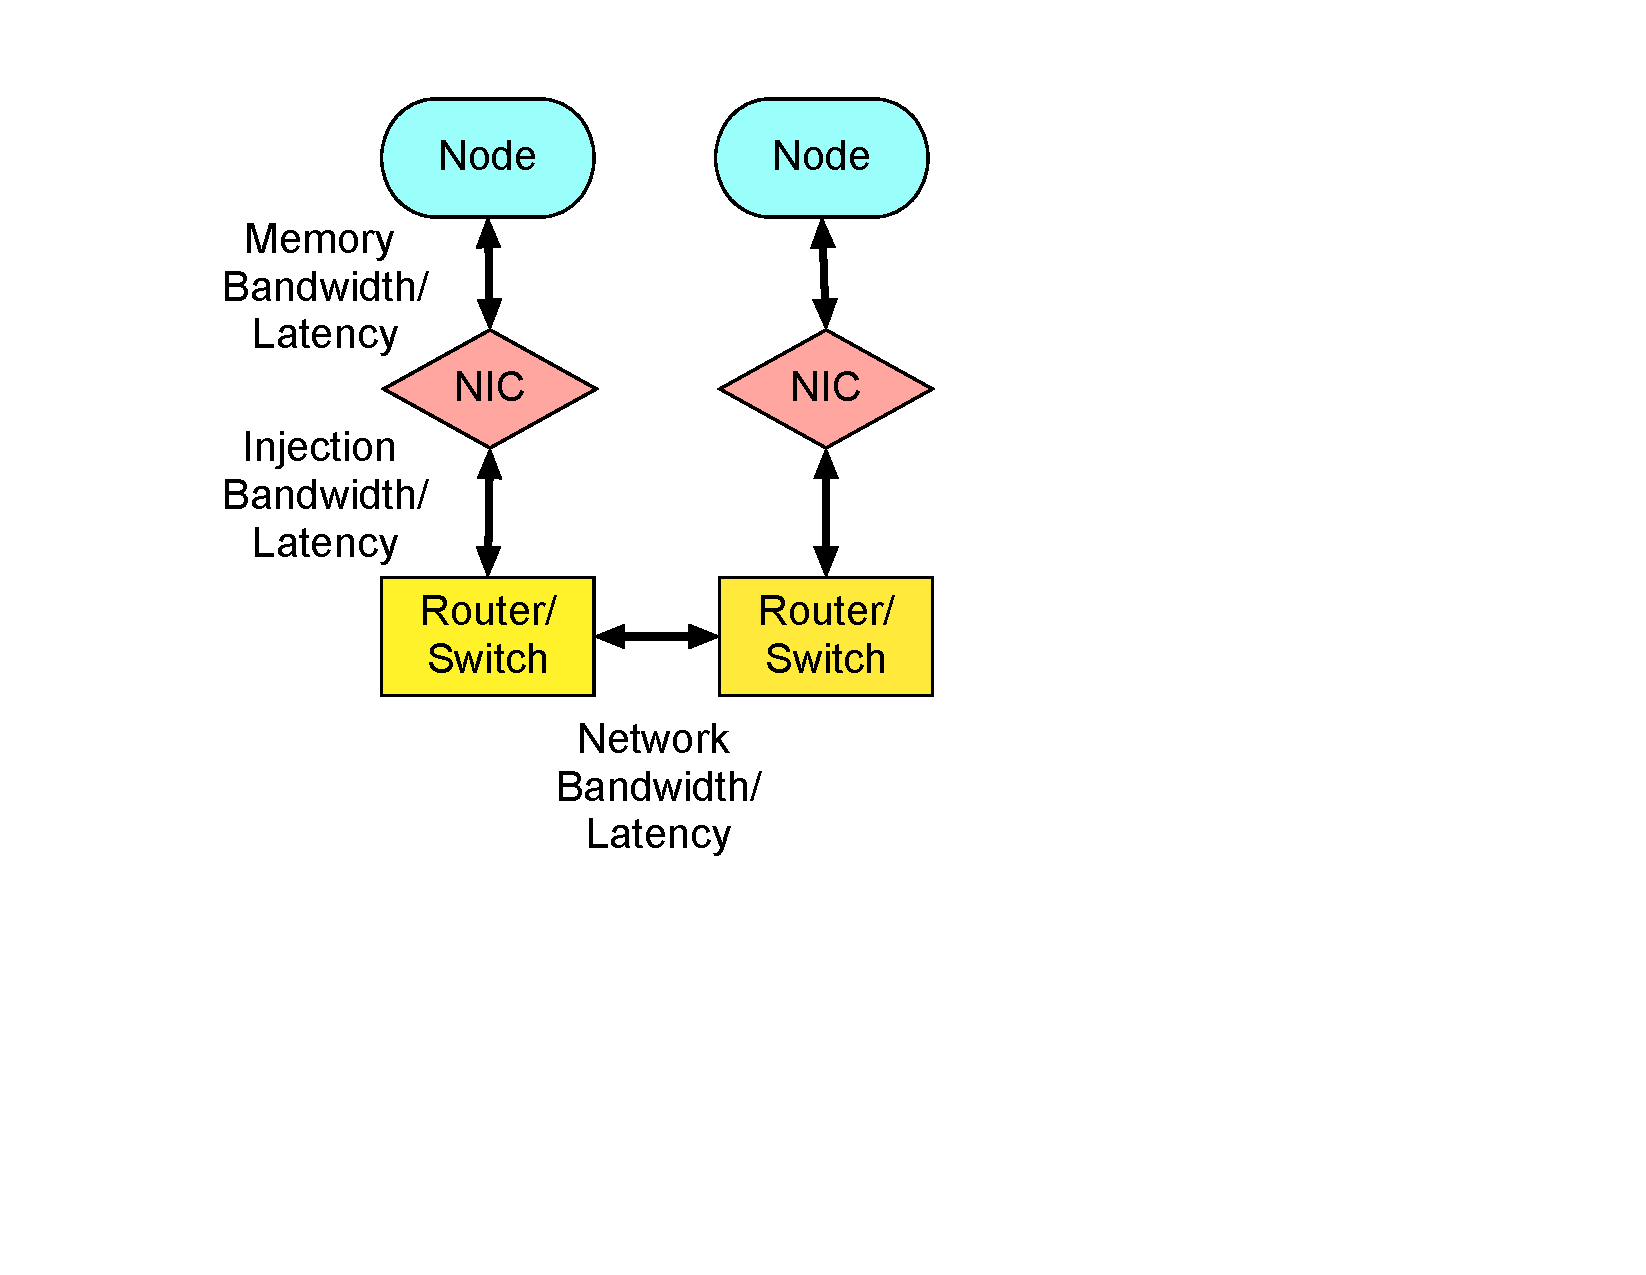
\includegraphics[width=0.4\textwidth]{figures/amm/AMM1.pdf}
\end{center}

This is simplest abstract machine model and incorporates three basic components (i.e. congestion points).
Each node has a memory subsystem and NIC (injection/ejection).
Once packets are injected, they traverse a series of network switches.
The memory, injection, and network are all defined by a bandwidth/latency parameter pair.

\begin{ViFile}
network_bandwidth = 6GB/s
network_hop_latency = 100ns
injection_bandwidth = 10GB/s
injection_latency = 1us
memory_bandwidth = 10GB/s
memory_latency = 15ns
\end{ViFile}

These are special parameters used by the AMM configurations.
They can be by-passed by directly using fully namespaced parameters (not shown).

NOTE: there is no parameter \inlinefile{network_latency}.
The parameter is \inlinefile{network_hop_latency}.
This is the latency required for a single packet to traverse one switch and hop to the next one in the network.
Thus, even in the most basic of network models, there is a still a notion of topology that affects the number of hops and therefore the latency.
To compute the total network network latency as one would observe in an MPI ping-ping benchmark, one would compute
\[
lat = n_{hops} * lat_{hop} + 2*lat_{inj}
\]
using the hop latency and the injection latency.

This abstract machine model is a good place to start for getting a ``lay of the land'' for simulations - and the simplest to configure.
However, it has a few deficiencies that can cause problems when there is serious memory or network congestion.
More details (and their fixes) are given in the next abstract machine models. 	

\subsection{AMM2}

\begin{center}
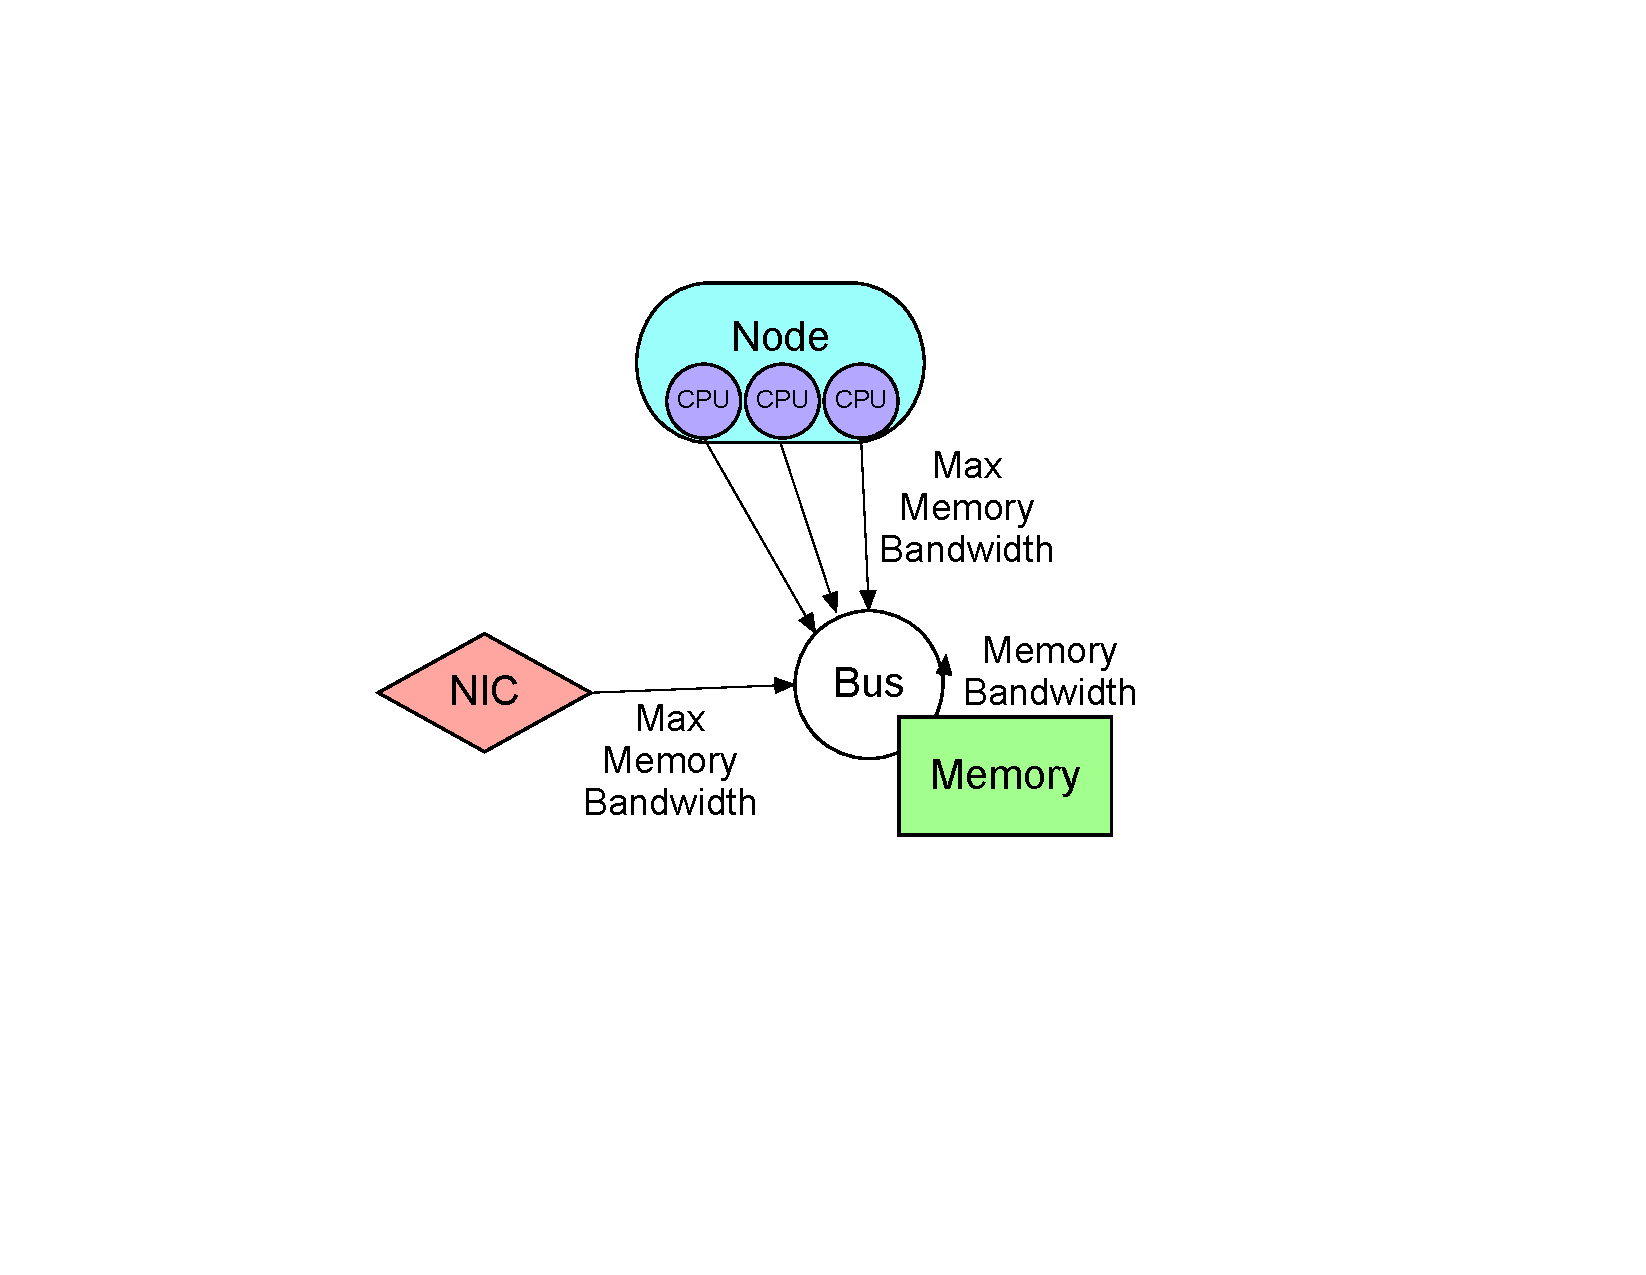
\includegraphics[width=0.4\textwidth]{figures/amm/amm2_membus.pdf}
\end{center}

\label{subsec:ammTwo}
A major deficiency of AMM1 is that it grants exclusive access to memory resources.
Two CPUs or the NIC cannot be using the memory subsystem in parallel.
This is particularly problematic for large memory transfers (1 MB or greater).
The memory system might be blocked for approx 1 ms,
creating unphysical delays while other resources wait for access.
A more realistic model allows multiple resources to access the memory,
albeit with reduced bandwidth when congestion is observed.
In many cases, multiple memory links or management units are connect to a shared bus.
The bus determines to the total, aggregate memory bandwidth.
However, the individual links determine the maximum observed bandwidth by any single component.
AMM2 has all the same parameters as AMM1, but now allows an additional parameter for memory.
These are special parameters used by the AMM configurations.
They can be by-passed by directly using fully namespaced parameters (not shown).

\begin{ViFile}
max_memory_bandwidth = 5GB/s
memory_bandwidth = 10GB/s
memory_latency = 15ns
\end{ViFile}
The new parameter \inlinefile{max_memory_bandwidth} now defines the maximum bandwidth any single component is allowed.
Thus, even if the CPU is doing something memory intensive, 5 GB/s is still available to the NIC for network transfers.
We remark here that the memory parameters might be named something slightly more descriptive.
However, as a rule, we want the AMM1 parameters to be a proper subset of the AMM2 parameters.
Thus parameter names should not change - only new parameters should be added.

\subsection{AMM3}
\label{subsec:ammThree}

\begin{center}
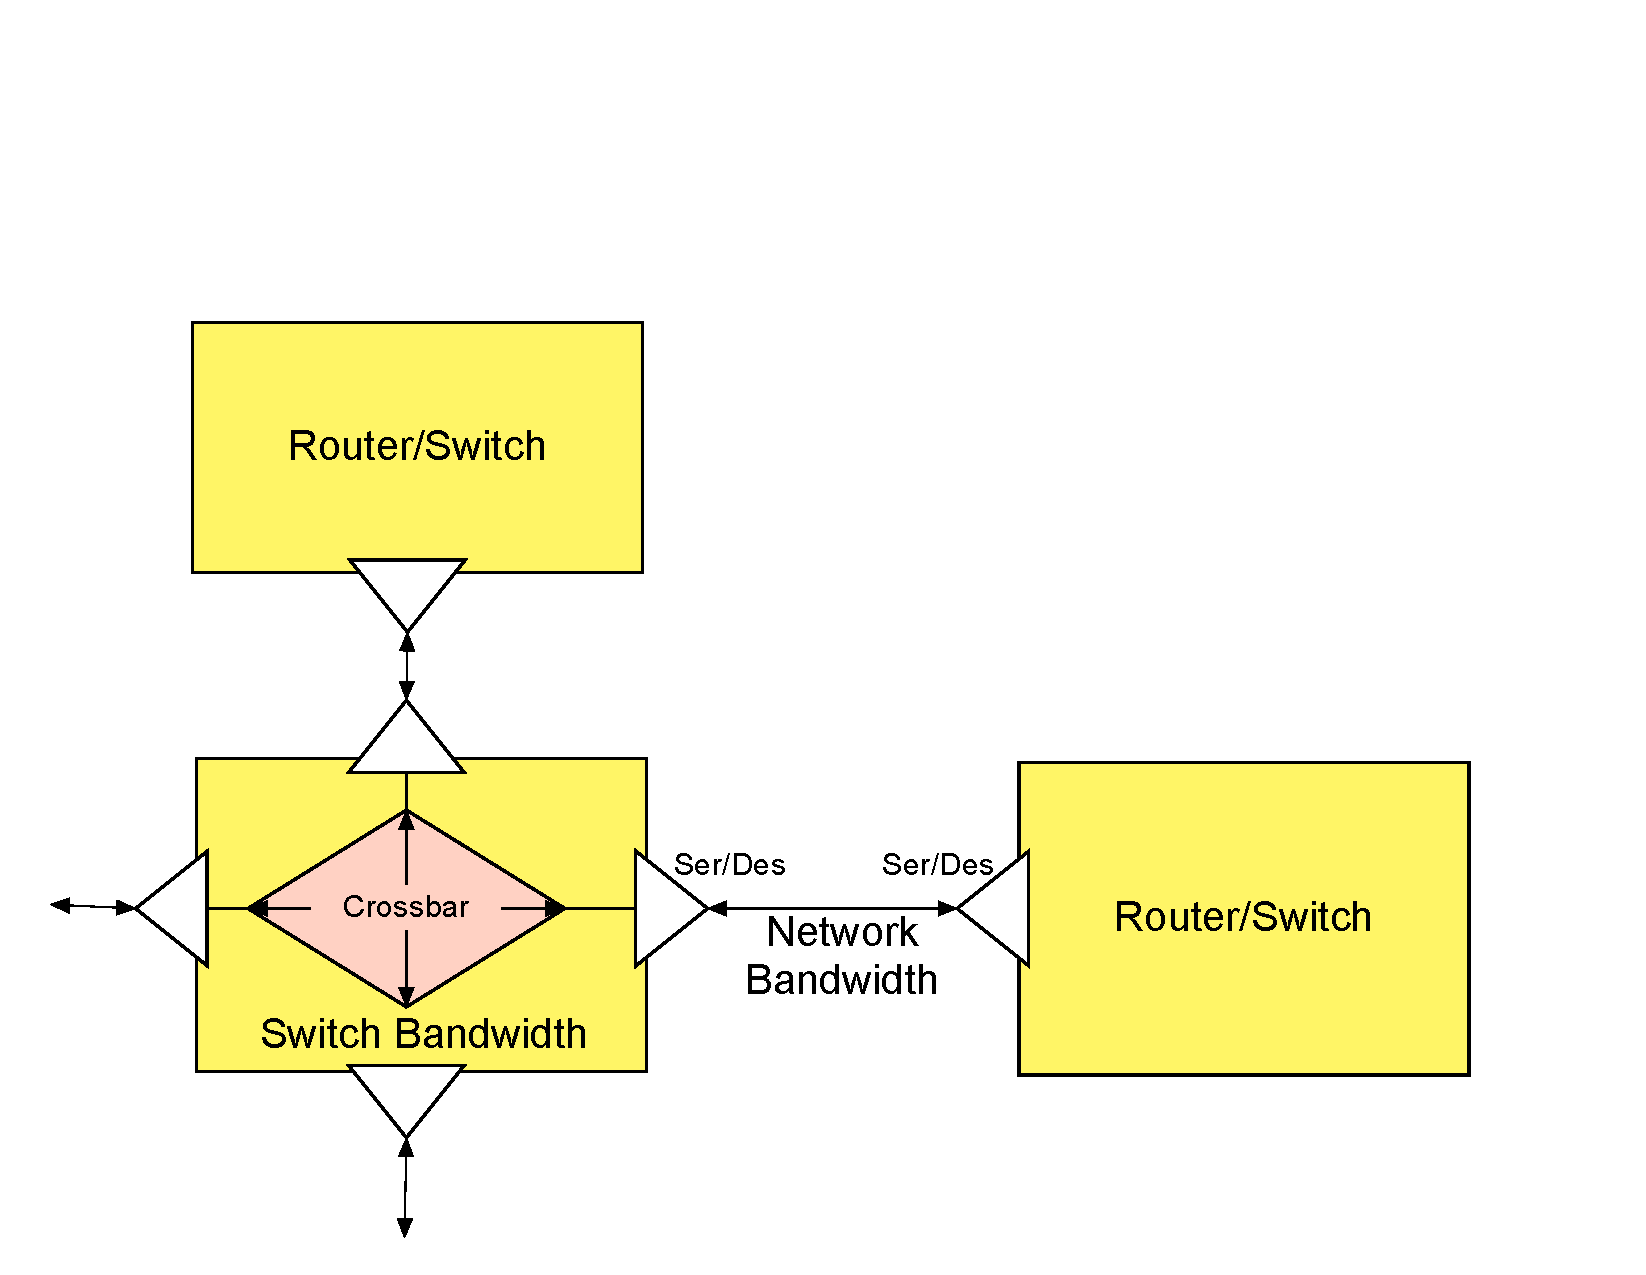
\includegraphics[width=0.5\textwidth]{figures/amm/amm3_switch.pdf}
\end{center}

A major deficiency of AMM2 is its inability to distinguish between the network link bandwidth (associated with the outport port serializer/deserializer) and the switch bandwidth (associated with the crossbar that arbitrates packets).  
Only packets traveling the same path cause congestion on the network links in AMM1 and AMM2.
However, packets ``intersecting'' at a switch - even if following separate paths - can cause congestion through sharing the switching fabric.
AMM3 generalize the network parameters by adding a switch bandwidth.
We note again here that AMM3 has all the same parameters as AMM2, plus the additional switch bandwidth parameter.
Thus, higher-numbered abstract machine models always add more detail.
These are special parameters used by the AMM configurations.
They can be by-passed by directly using fully namespaced parameters (not shown) for more detailed configurations.

\begin{ViFile}
network_switch_bandwidth = 12GB/s
network_bandwidth = 6GB/s
network_hop_latency = 100ns
\end{ViFile}

%% !TEX root = manual.tex

\section{Network Topologies and Routing}
\label{sec:tutorial:topology}
We here give a brief introduction to specifying different topologies and routing strategies.  
We will only discuss one basic example (torus).  
A more thorough introduction covering all topologies is planned for future releases.
Excellent resources are ``Principles and Practices of Interconnection Networks'' by Brian Towles and William Dally published by Morgan Kaufman and ``High Performance Datacenter Networks'' by Dennis Abts and John Kim published by Morgan and Claypool.

\subsection{Topology}
\label{subsec:tutorial:topology}

Topologies are determined by two mandatory parameters.
\begin{ViFile}
topology.name = torus
topology.geometry = 4 4
\end{ViFile}
Here we choose a 2D-torus topology with extent 4 in both the $X$ and $Y$ dimensions for a total of 16 nodes (Figure \ref{fig:hdtorus:basic})
The topology is laid out in a regular grid with network links connecting nearest neighbors.  
Additionally, wrap-around links connect the nodes on each boundary.  
\begin{figure}[h]
\centering
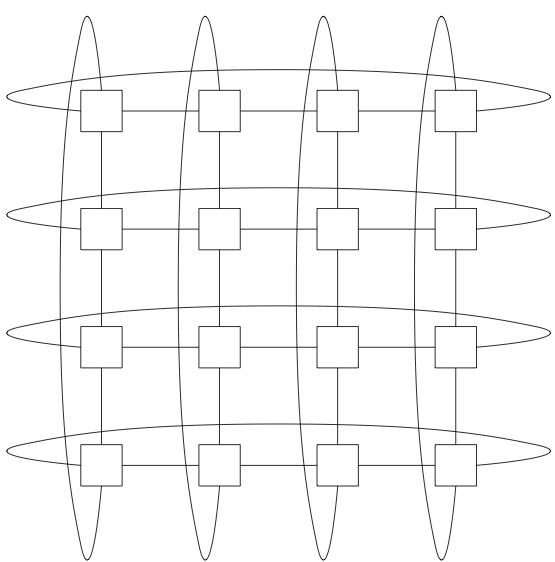
\includegraphics[width=0.5\textwidth]{figures/tikz/torus/torus.png}
\caption{4 x 4 2D Torus}
\label{fig:hdtorus:basic}
\end{figure}


The figure is actually an oversimplification.  
The \inlinefile{topology_geometry} parameter actually specifies the topology of the \emph{network switches}, not the compute nodes. 
A torus is an example of a direct network in which each switch has one or more nodes ``directly'' connected to it.  
A more accurate picture of the network is given in Figure \ref{fig:hdtorus:withnodes}.
\begin{figure}[h]
\centering
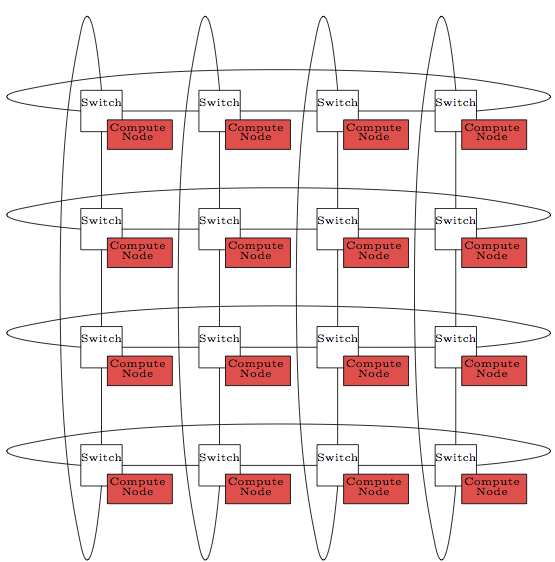
\includegraphics[width=0.4\textwidth]{figures/tikz/torus/withnodes.png}
\caption{4 x 4 2D Torus of Network Switches with Compute Nodes}
\label{fig:hdtorus:withnodes}
\end{figure}
While in many previous architectures there was generally a one-to-one correspondence between compute nodes and switches, more recent architectures have multiple compute nodes per switch (e.g. Cray Gemini with two nodes).  
Multinode switches can be specified via

\begin{ViFile}
topology.name = torus
topology.geometry = 4 4
topology.concentration = 2
\end{ViFile}
which would now generate a torus topology with 16 switches and 32 compute nodes.

Another subtle modification of torus (and other networks) can be controlled by giving the $X$, $Y$, and $Z$ directions different bandwidth.  
The above network could be modified as

\begin{ViFile}
topology.name = torus
topology.geometry = 4 4
topology.redundant = 2 1
\end{ViFile}
giving the the $X$-dimension twice the bandwidth of the $Y$-dimension.  
This pattern DOES exist in some interconnects as a load-balancing strategy.  
A very subtle point arises here. Consider two different networks:

\begin{ViFile}
topology.name = torus
topology.geometry = 4 4
topology.redundant = 1 1
network_bandwidth = 2GB/s
\end{ViFile}
\begin{ViFile}
topology.name = torus
topology.geometry = 4 4
topology.redundant = 2 2
network_bandwidth = 1GB/s
\end{ViFile}
For some coarse-grained models, these two networks are exactly equivalent.  
In more fine-grained models, however, these are actually two different networks.  
The first network has ONE link carrying 2 GB/s. The second network has TWO links each carrying 1 GB/s.

\subsection{Routing}
\label{subsec:tutorial:routing}
By default, \sstmacro uses the simplest possible routing algorithm: dimension-order minimal routing (Figure \ref{fig:torus:basicrouting}).
\begin{figure}[h]
\centering
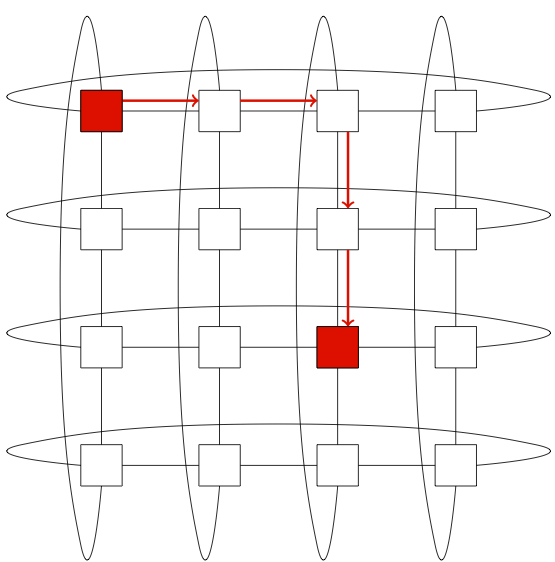
\includegraphics[width=0.4\textwidth]{figures/tikz/torus/minroutetorus.png}
\caption{Dimension-Order Minimal Routing on a 2D Torus}
\label{fig:torus:basicrouting}
\end{figure}
In going from source to destination, the message first travels along the $X$-dimension and then travels along the $Y$-dimension.
The above scheme is entirely static, making no adjustments to avoid congestion in the network.  
\sstmacro supports a variety of adaptive routing algorithms.  This can be specified:

\begin{ViFile}
router = min_ad
\end{ViFile}
which specifies minimal adaptive routing. 
There are now multiple valid paths between network endpoints, one of which is illustrated in Figure \ref{fig:torus:minadrouting}.
\begin{figure}[h!]
\centering
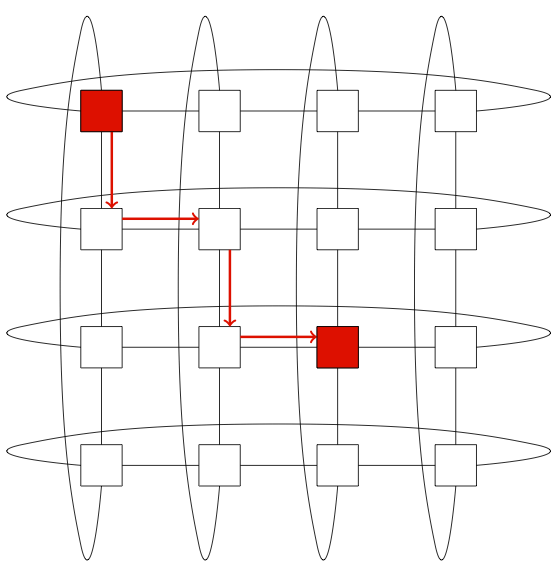
\includegraphics[width=0.4\textwidth]{figures/tikz/torus/minadroutetorus.png}
\caption{Adaptive Minimal Routing on a 2D Torus}
\label{fig:torus:minadrouting}
\end{figure}
At each network hop, the router chooses the \emph{productive} path with least congestion.  
In some cases, however, there is only one minimal path (node $(0,0)$ sending to $(2,0)$ with only $X$ different).
For these messages, minimal adaptive is exactly equivalent to dimension-order routing.  
Other supported routing schemes are valiant and UGAL.  More routing schemes are scheduled to be added in future versions.  
A full description of more complicated routing schemes will be given in its own chapter in future versions. 
For now, we direct users to existing resources such as ``High Performance Datacenter Networks'' by Dennis Abts and John Kim.

%% !TEX root = manual.tex

\section{Network Model}
\label{sec:tutorial:networkmodel}

Network models can be divided into several categories.  SST/macro supports analytic models, which estimate network delays via basic latency/bandwidth formulas, and packet models, which model step-by-step the transit of individuals through the interconnect.
A third class of models (flow models), was previously supported but are now discontinued due to the much better scalability of packet models.

\subsection{Analytic Models: MACRELS}
\label{subsec:tutorial:macrels}

The analytic models in SST/macro are colloqiually referred to as MACRELS (MTL for AnalytiC REally Lightweight Simulation).
An example file running a simple application can be found in the top-level examples folder.
The MTL (message transfer layer) moves entire network flows from point-to-point without packetizing them into smaller chunks.
Thus an entire 1 MB MPI message is transported as a single chunk of data.  
The majority of MACRELS models are based on the LogP set of approximations:

\[
\Delta t = \alpha + \beta N
\]
where $\Delta t$ is the time delay, $\alpha$ is the minimum latency of the communication, $\beta$ is the inverse bandwidth (s/B), and N is the number of bytes.
In abstract machine models, these methods are selected as:

\begin{ViFile}
congestion_model = logP
\end{ViFile}
Details are shown for traffic moving from source to destination in Figure \ref{fig:macrelsOverview}.
Modeling occurs on entire flows, rather than individual packets. 

\begin{enumerate}
\item Flows queue waiting for NIC injection link to become available. Flow is forwarded to destination NIC based after computed delay. 
\item Flows queue waiting for NIC ejection link to become available. Flow finishes after ejection link becomes available.
\end{enumerate}

\begin{figure}
\centering
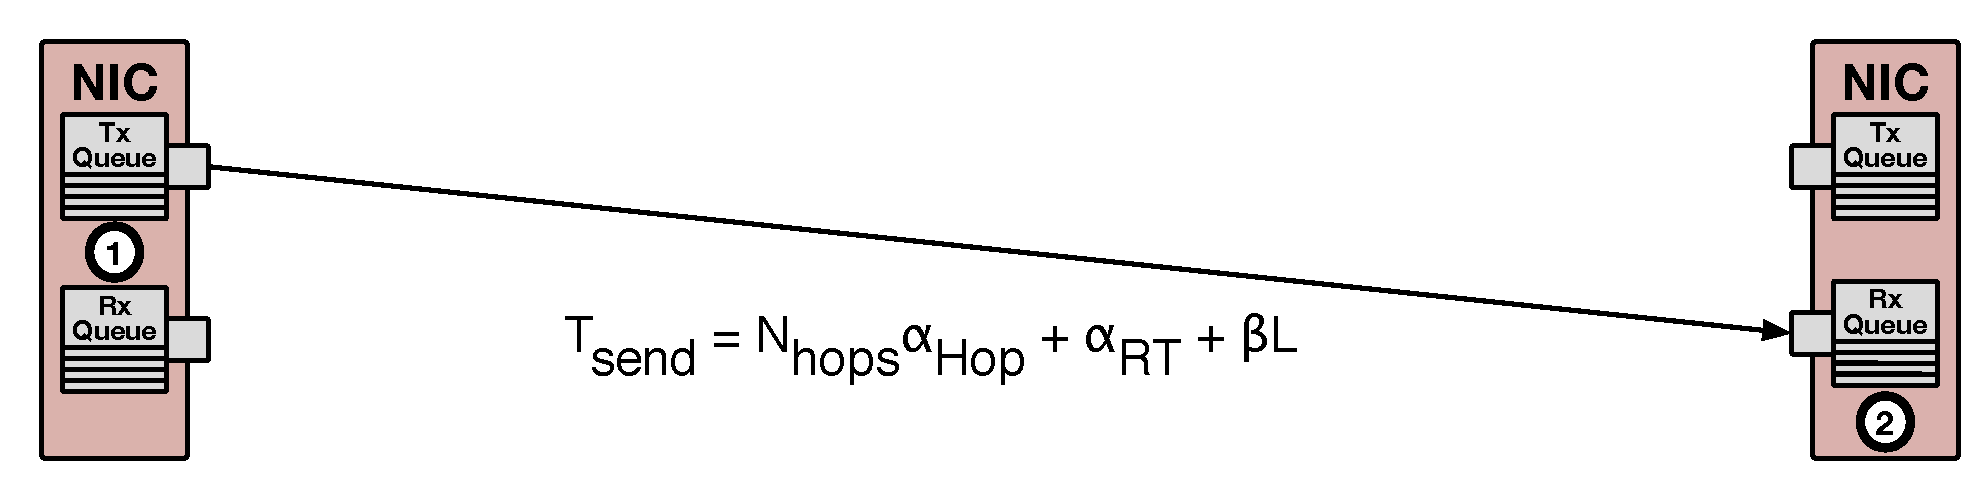
\includegraphics[width=0.9\textwidth]{figures/macrels.pdf}
\caption{MACRELS (Messages with AnalytiC REally Lightweight Simulation) skips congestion modeling and approximates send delays using a simple latency/bandwidth estimate, similar to the LogGOP model. Modeling occurs on entire flows, rather than individual packets. For details on numbered steps, see text.}
\label{fig:macrelsOverview}
\end{figure}


\subsection{Packet Models: PISCES}
\label{subsec:tutorial:pisces}

PISCES (Packet-flow Interconnect Simulation for Congestion at Extreme Scale) breaks network flows (MPI messages) into individual packets and models each packet individually.
An example file running a simple application can be found in the top-level examples folder.
In reality, packets are further subdivided into flits (flow-control units).
Flit-level detail would be way too computationally intense for large-scale simulation.
All routing decisions are made on packets as a while. 
Two flits in the same packet cannot take different paths through the network.
However, they may not travel together.

PISCES (Packet-flow Interconnect Simulation for Congestion at Extreme-Scale) models individual packets moving through the network. Flits (flow-control units) are approximately modeled using flow-like approximations. Packets can have partial occupancies in several different buffers, approximating wormhole routing. However, arbitration is modeled on whole packets, not individual flits (see Figure \ref{fig:piscesOverview})
\begin{enumerate}
\item A message (flow) is broken up into packets. Depending on available space in the Tx buffer, a limited number of packets may be able to queue up in the buffer. If credits are available in the Rx buffer for the link and the link is idle, the packet moves into the next Rx buffer after a computed delay.
\item The router selects a path for the packet and the packet requests to the crossbar to transmit to the corresponding output port. If credits are available for the Rx buffer, the crossbar may select the packet in arbitration and move it to the output buffer. After moving, the Rx buffer returns credits to the previous Tx buffer for that packet.
\item Step 1 is repeated for the next Rx buffer, waiting for credits and link availability.
\item Repeat Step 2
\item Repeat Step 3
\item Packet arrives in NIC Rx queue and queues waiting to inject into local memory. After injection, the Rx buffer returns credits to the corresponding Tx buffer.
\end{enumerate}

\begin{figure}[h!]
\centering
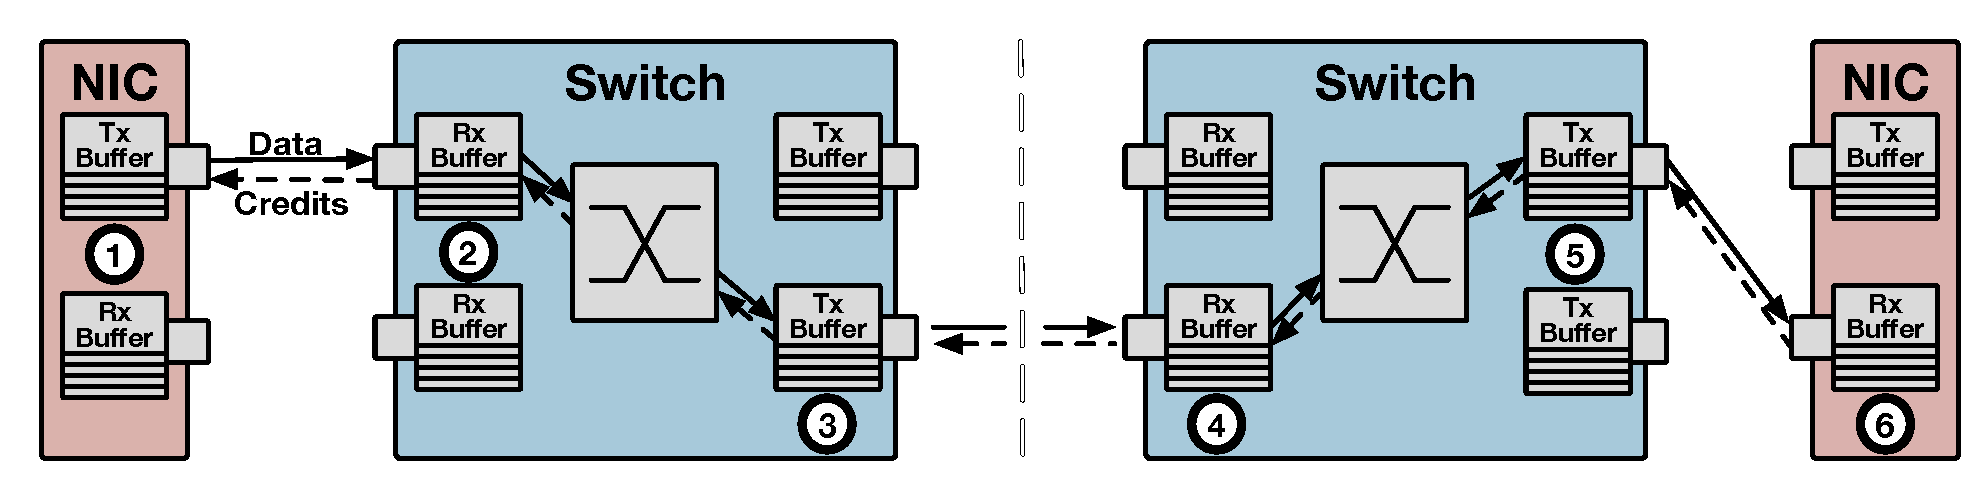
\includegraphics[width=0.9\textwidth]{figures/pisces_overview.pdf}
\caption[PISCES model]{PISCES (Packet-flow Interconnect Simulation for Congestion at Extreme-Scale) models individual packets moving through the network. Flits (flow-control units) are approximately modeled using flow-like approximations. For details on numbered steps, see text.}
\label{fig:piscesOverview}
\end{figure}


PISCES provides two mechanisms for treating flit-level flow control discussed next.

\subsubsection{PISCES simple model}
\label{subsubsec:tutorial:simplePisces}
In the simple model, each router uses a basic store-and-forward mechanism.
Flits are not allowed to ``separate'' and always travel as a single unit.
The entire packet has to be stored within a router before it can be forwarded to the next router.
The simple model affects the arbitrator that decided when and how to transmit flits.
To select a simple model:

\begin{ViFile}
arbitrator = simple
\end{ViFile}
The simple model is the least computationally expensive. 
However, for large packet sizes, it can produce erroneously high latencies.
To tune the packet size for abstract machine models, set:

\begin{ViFile}
switch.mtu = 1024B
node.nic.mtu = 1024B
\end{ViFile}
which sets the packet size to 1024B. 
For the simple model, packet sizes larger than 256-512B are not recommended.
Packet sizes on production supercomputers are often small (96-128B).
Small packet sizes with the simple model can be a good compromise for having more fine-grained routing but cheaper congestion modeling in the arbitrator.
More details are given in Figure \ref{fig:piscesOverview}.

\subsubsection{PISCES cut-through model}
\label{subsubsec:tutorial:cutThroughPisces}

\begin{figure}
\centering
\includegraphics[width=0.6\textwidth]{figures/pisces}
\caption{Timeline of four different packets passing through a PISCES cut-through bandwidth arbitrator. The incoming bandwidth (I) and outgoing bandwidth (O) are shown for each packet.  Time is the horizontal axis. Bandwidth consumed by a packet is shown by the vertical extent of each packet. The individual events are 1) First packet arrives 2) Second packet arrives with reduced bandwidth but no available bandwidth 3) First packet finishes. Second packet can begin sending. 4) Third packet arrives and begins sending with remaining bandwidth. 5) Fourth packet arrives, but no available bandwidth. 6) Second packet finishes. Third packet increases bandwidth. Fourth packet can begin sending. 7) Third packet finishes. Fourth packet increases bandwidth. 8) Fourth packet finishes.
Full details are given in the text.}
\label{fig:pisces}
\end{figure}

In the cut-through model, routing decisions still occur at the packet-level.
However, some attempt is made to account for pipelining of flits across different router stages.
Somewhat similar to the LogP models used above, latency/bandwidth formulas are used to estimate packet delays.
However, the cut-through model adds more details.
It's requested as:

\begin{ViFile}
arbitrator = cut_through
\end{ViFile}
Figure \ref{fig:pisces} shows a timeline for the data being transmitted through a crossbar, SerDes, or other network component with a ``fixed bandwidth.'' 
Each component is essentially a pipe with some flow bandwidth.
The arbitrator divides its limited bandwidth amongst incoming packets.
Packets fill the pipeline, consuming bandwidth.
In contrast to the completely discrete simple model, packets can ``multiplex'' in the component sharing an arbitrary bandwidth partition.
Modeling a packet delay starts with two input parameters and computes three output parameters.

\begin{itemize}
\item $A$: Packet head arrival (input)
\item $I$: Packet incoming bandwidth (input)
\item $H$: Packet head departure (output)
\item $T$: Packet tail departure (output)
\item $O$: Packet outgoing bandwidth (output)
\end{itemize}

In the simple model, a packet either consumes all the bandwidth or none of the bandwidth.
To account for flit-level pipelining, the cut-through model allows packets to consume partial bandwidths.
Consider an aribitrator that has a maximum bandwidth of 1.0.
The first packet (purple, Figure \ref{fig:pisces}) arrives with a full incoming bandwidth of 1.0 and head arrival of t=0.0.
It therefore consumes all the available bandwidth. 
The head of the packet can actually leave immediately (as it must to properly pipeline or cut-through).
The tail leaves after all bytes have sent at t=1.0.
Thus for the first packet we have $H$=0.0, $T$=1.0, and $O$=1.0.

The second packet (orange) arrives at t=0.5. 
Upon arrival there is no bandwidth available as the first packet is consuming the maximum.
Only after the first packet finishes can the second packet begin.
The second packet arrives and leaves with a reduced bandwidth of 0.5. 
Thus we have $H$=1.0, $T$=3.0, and $O$=0.5.

The third packet (green) arrives at t=1.75.
Upon arrival there is some bandwidth, but not enough to match the incoming bandwidth of 0.57.
Thus the third packet is slowed initially.
After the second packet finished, the third packet can send at increased bandwidth.
The computation here is a bit more complicated.
Packet 3 can actually consume MORE than 0.6 bandwidth units.
Between steps 4 and 6, packet 3 has accumulated in a local buffer in the router.
Thus even though the incoming bandwidth is only 0.6, there are several flits that are available to send immediately at full bandwidth waiting in the buffer.
Thus results in an effective bandwidth of 0.75 for the remainder of the packet's time in the arbitrator.
Thus we end up with $H$=1.75, $T$=3.5, and $O$=0.57.
Even though the packet is initially delayed, the buffers compensate for the delay and allow the outgoing bandwidth to ``catch up'' with the incoming bandwidth.

Finally, the fourth packet (blue) arrives at t=3.0. 
There is some available bandwidth. After the third packet finishes, the fourth packet can now send at maximum.
Because of the initial delay, the outgoing bandwidth is somewhat reduced.
We have $H$=3.0, $T$=4.38, and $O$=0.73.

\subsection{SCULPIN}
Under current architectural trends, switches have ample buffer space and crossbar bandwidth, making the mostly likely bottleneck edge bandwidth through the output ports.
An example file running a simple application can be found in the top-level examples folder.
SCULPIN (Simple Congestion Unbuffered Latency Packet Interconnection Network) models the main source of contention in today's networks occurring on the output port ser/des. Unlike PISCES, individual flits are not able to wormhole route across links interspersed with flits from other packets.
\begin{enumerate}
\item A message (flow) is broken up into packets. Each packet waits in the queue to send based on link availability and QoS.
\item After being selected, the packets are forwarded to the switch. Packets are immediately routed to the correct output port, skipping crossbar arbitration. Packets wait in unbounded queues, thereby assuming sufficient buffer space is always available.
\item Repeat Step 1. Packet waits in queue until link becomes available based on QoS. Packet is immediately forwarded to next output port, skipping arbitration
\item Repeat Step 1.
\item Packet arrives in NIC Rx queue (no credits, buffer assumed to always have space). Packets queue waiting to inject into local memory.
\end{enumerate}

\begin{figure}
\centering
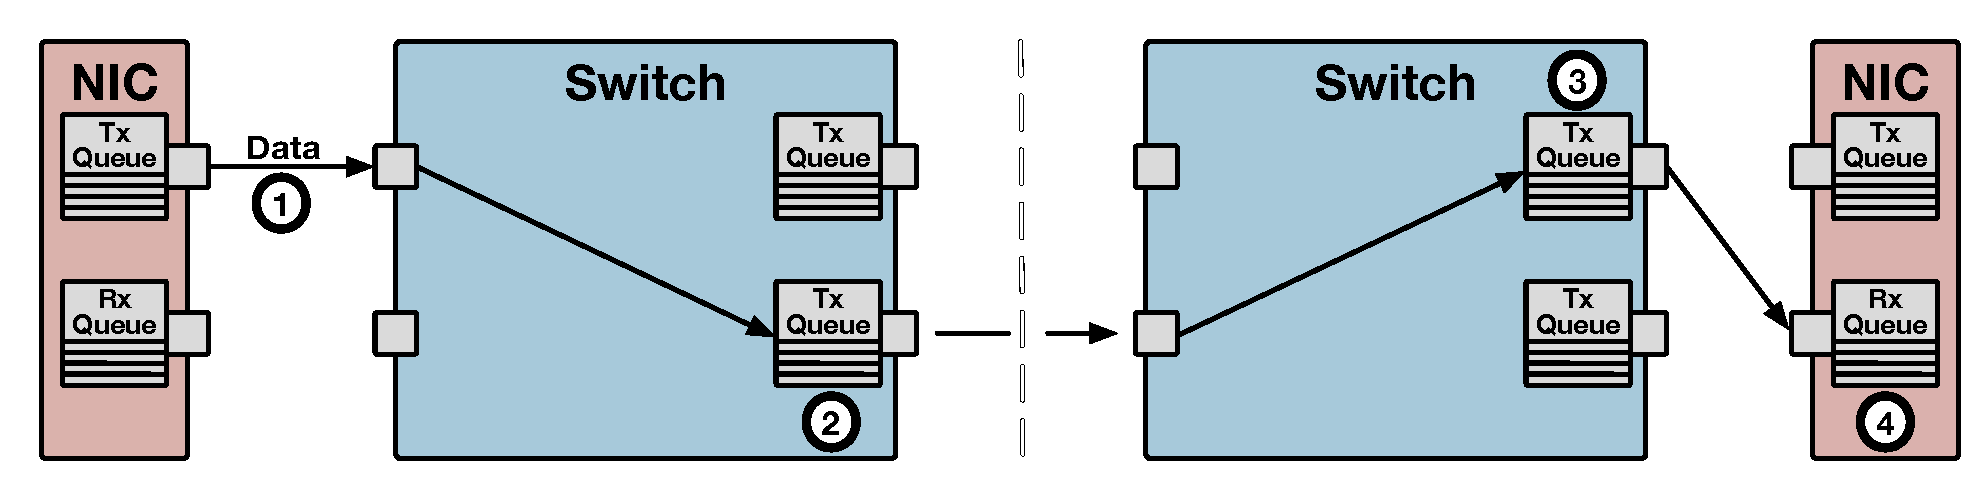
\includegraphics[width=0.9\textwidth]{figures/sculpin.pdf}
\caption[SCULPIN model]{SCULPIN (Simple Congestion Unbuffered Latency Packet Interconnection Network) models the main source of contention in today's networks occurring on the output port ser/des. For details on numbered steps, see text.}
\label{fig:sculpin}
\end{figure}

\subsection{SNAPPR}
Because of the coarse-grained mechanisms used in PISCES and SCULPIN, it can be difficult to model more advanced mechanisms like QoS or congestion control. 
SNAPPR (Simulator Network for Adaptive Priority Packet Routing) uses a coarse-grained cycle-based simulation that allows priority queues based on QoS or restricting injection rate for congestion control. The model is configured in much the same way as the other models.  SNAPPR is slightly more expensive than the other models, but provides by far the most flexibility and most detailed statistics.
An example file running a simple application can be found in the top-level examples folder.

\subsection{Flow}
\label{subsec:tutorial:flow}
The flow model, in simple cases, corrects the most severe problems of the packet model.
Instead of discrete chunks, messages are modeled as fluid flows moving through the network.
Congestion is treated as a fluid dynamics problem, sharing bandwidth between competing flows.
In contrast to LogP models, flow models can account fairly well for congestion.
Without congestion, a flow only requires a FLOW START and FLOW STOP event to be modeled (see tutorial on discrete event simulation in \ref{sec:tutorial:des}).
While the packet model would require many, many events to simulate a 1 MB message, the flow model might only require two.
With congestion, flow update events must be scheduled whenever congestion changes on a network link.  
For limited congestion, only a few update events must occur.
The flow model also corrects the latency and multiplexing problems in the PISCES simple model, providing higher-accuracy for coarse-grained simulation.

The flow model starts to break down for large systems or under heavy congestion.
In the packet model, all congestion events are ``local'' to a given router.  
The number of events is also constant in packet models regardless of congestion since we are modeling a fixed number of discrete units.
In flow models, flow update events can be ``non-local,'' propagating across the system and causing flow update events on other routers.
When congestion occurs, this ``ripple effect'' can cause the number of events to explode, overwhelming the simulator.
For large systems or heavy congestion, the flow model is actually much slower than the packet model. Support for this model has been completely removed.



%% !TEX root = manual.tex

\section{Basic MPI Program}
\label{sec:tutorial:basicmpi}
Let us go back to the simple send/recv skeleton and actually look at the code.  
This code should be compiled with SST compiler wrappers installed in the \inlineshell{bin} folder.

\begin{CppCode}
#include <stdlib.h>
#include <stdio.h>
#include <mpi.h>

int main(int argc, char **argv) 
{
  int message_size = 128;
  int me, nproc;
  int tag = 0;
  int dst = 1;
  int src = 0;
  MPI_Status stat;

  MPI_Init(&argc,&argv);
  MPI_Comm world = MPI_COMM_WORLD;
  MPI_Comm_rank(world,&me);
  MPI_Comm_size(world,&nproc);
\end{CppCode}
The starting point is creating a main routine for the application.
The simulator itself already provides a \inlinecode{main} routine.
The SST compiler automatically changes the function name to \inlinecode{userSkeletonMain},
which provides an entry point for the application to actually begin.
When \sstmacro launches, it will invoke this routine and pass in any command line arguments specified via the \inlinefile{app1.argv} parameter.  Upon entering the main routine, 
the code is now indistinguishable from regular MPI C++ code.  
In the parameter file to be used with the simulation, you must set

\begin{ViFile}
node {
 app1 {
  exe = <PATH_TO_EXE>
\end{ViFile}

While MPI would have produced an executable, SST works by loading shared object files using \inlinecode{dlopen}.
To get SST to load the skeleton, you must specify the path of the ``executable" in the input file.
Using \inlinecode{dlopen} tricks, SST finds the main function in the .so file and calls it to spawn the skeleton app.
Just as an executable can only have one main, SST shared object files can only have a single executable in them at a time.

At the very top of the file, the \inlineshell{mpi.h} header is actually mapped by the SST compiler to an \sstmacro header file.
This header provides the MPI API and configures MPI function calls to link to \sstmacro instead of the real MPI library.  
The code now proceeds:

\begin{CppCode}
  if (nproc != 2) {
    fprintf(stderr, "sendrecv only runs with two processors\n");
      abort();
  }
  if (me == 0) {
    MPI_Send(NULL, message_size, MPI_INT, dst, tag, world);
    printf("rank %i sending a message\n", me);
  }
  else {
    MPI_Recv(NULL, message_size, MPI_INT, src, tag, world, &stat);
    printf("rank %i receiving a message\n", me);
  }
  MPI_Finalize();
  return 0;
}
\end{CppCode}
Here the code just checks the MPI rank and sends (rank 0) or receives (rank 1) a message.

For more details on what exactly the SST compiler wrapper is doing, you can specify \inlineshell{SSTMAC_VERBOSE=1} as an environment variable to have SST print out detailed commands. Additionally, you can specify \inlineshell{SSTMAC_DELETE_TEMPS=0} to examine any temporary source-to-source files.

\subsection{DEPRECATED: App name macro}
Previously, applications had to be ``named'' by using the \inlinecode{sstmac_app_name} macro.
This macro can still be define just above main to give a descriptive name to the skeleton:

\begin{CppCode}
#include <mpi.h>

#define sstmac_app_name simple_test

int main(int argc, char **argv) 
{
\end{CppCode}

This was previously required for starting applications, but now is only used
for providing descriptive labels for certain applications.
It is not recommended for use anymore and is ignored. An equivalent naming can just be provided by:

\begin{ViFile}
node {
 app1 {
   exe = <PATH_TO_EXE>
   name = simple_test
 }
}
\end{ViFile}




%% !TEX root = manual.tex

\section{Launching, Allocation, and Indexing}
\label{sec:tutorial:launchetc}

\subsection{Launch Commands}
\label{subsec:tutorial:launch}
Just as jobs must be launched on a shared supercomputer using Slurm or aprun, 
SST/macro requires the user to specify a launch command for the application.
Currently, we encourage the user to use aprun from Cray, for which documentation can easily be found online.
In the parameter file you specify, e.g.

\begin{ViFile}
app1.name = user_mpiapp_cxx
app1.launch_cmd = aprun -n 8 -N 2
\end{ViFile}
which launches an external user C++ application with eight ranks and two ranks per node.
The aprun command has many command line options (see online documentation), some of which may be supported in future versions of SST/macro.  In particular, we are in the process of adding support for thread affinity, OpenMP thread allocation, and NUMA containment flags.  Most flags, if included, will simply be ignored.

\subsection{Allocation Schemes}
\label{subsec:tutorial:allocation}
In order for a job to launch, it must first allocate nodes to run on. Here we choose a simple 2D torus

\begin{ViFile}
topology.name = torus
topology.geometry = 3 3
topology.concentration = 1
\end{ViFile}
which has 9 nodes arranged in a 3x3 mesh.  
For the launch command \inlinefile{aprun -n 8 -N 2}, we must allocate 4 compute nodes from the pool of 9.
Our first option is to specify the first available allocation scheme (Figure \ref{fig:allocation:first_available})

\begin{ViFile}
app1.launch_allocation = first_available
\end{ViFile}
\begin{figure}[h]
\centering
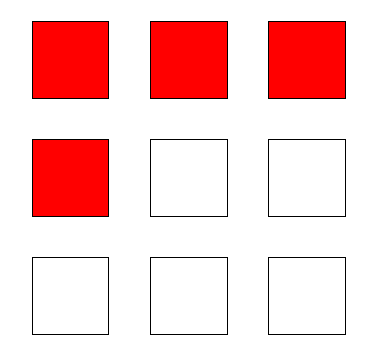
\includegraphics[width=0.35\textwidth]{figures/tikz/allocation/firstavailable.pdf}
\caption{First available Allocation of 4 Compute Codes on a 3x3 2D Torus}
\label{fig:allocation:first_available}
\end{figure}
In first available, the allocator simply loops through the list of available nodes as they are numbered by the topology object.
In the case of a 2D torus, the topology numbers by looping through columns in a row.
In general, first available will give a contiguous allocation, but it won't necessarily be ideally structured.

To give more structure to the allocation, a Cartesian allocator can be used (Figure \ref{fig:allocation:cartesian}).

\begin{ViFile}
app1.launch_allocation = cartesian
app1.cart_launch_sizes = 2 2
app1.cart_launch_offsets = 0 0
\end{ViFile}
\begin{figure}[h]
\centering
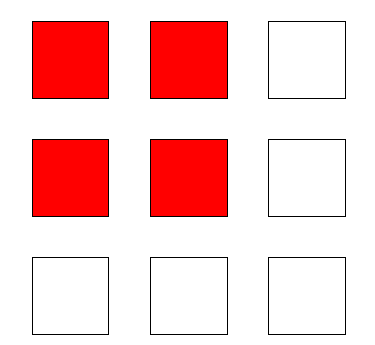
\includegraphics[width=0.35\textwidth]{figures/tikz/allocation/cartesian.pdf}
\caption{Cartesian Allocation of 4 Compute Codes on a 3x3 2D Torus}
\label{fig:allocation:cartesian}
\end{figure}
Rather than just looping through the list of available nodes, we explicitly allocate a 2x2 block from the torus.
If testing how ``topology agnostic'' your application is, you can also choose a random allocation.

\begin{ViFile}
app1.launch_allocation = random
\end{ViFile}
\begin{figure}[h]
\centering
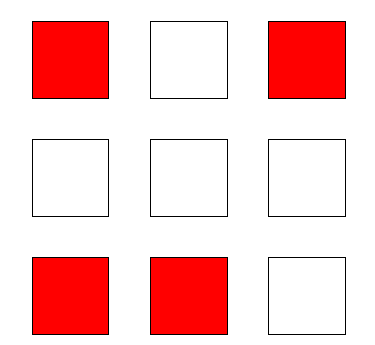
\includegraphics[width=0.35\textwidth]{figures/tikz/allocation/random.pdf}
\caption{Random Allocation of 4 Compute Codes on a 3x3 2D Torus}
\label{fig:allocation:random}
\end{figure}

In many use cases, the number of allocated nodes equals the total number of nodes in the machine.
In this case, all allocation strategies allocate the same \emph{set} of nodes, i.e. the whole machine.
However, results may still differ slightly since the allocation strategies still assign an initial numbering of the node,
which means a random allocation will give different results from Cartesian and first available.


\subsubsection{Indexing Schemes}
\label{subsec:tutorial:indexing}
Once nodes are allocated, the MPI ranks (or equivalent) must be assigned to physical nodes, i.e. indexed.
The simplest strategies are block and round-robin.  If only running one MPI rank per node, the two strategies are equivalent,
indexing MPI ranks in the order received from the allocation list.
If running multiple MPI ranks per node, block indexing tries to keep consecutive MPI ranks on the same node (Figure \ref{fig:indexing:block}).

\begin{ViFile}
app1.launch_indexing = block
\end{ViFile}
\begin{figure}[h]
\centering
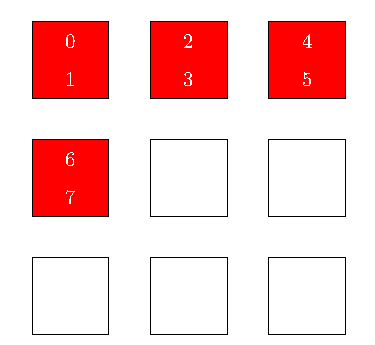
\includegraphics[width=0.4\textwidth]{figures/tikz/indexing/block.pdf}
\caption{Block Indexing of 8 MPI Ranks on 4 Compute Nodes}
\label{fig:indexing:block}
\end{figure}
In contrast, round-robin spreads out MPI ranks by assigning consecutive MPI ranks on different nodes (Figure \ref{fig:indexing:round_robin}).

\begin{ViFile}
app1.launch_indexing = round_robin
\end{ViFile}
\begin{figure}[h]
\centering
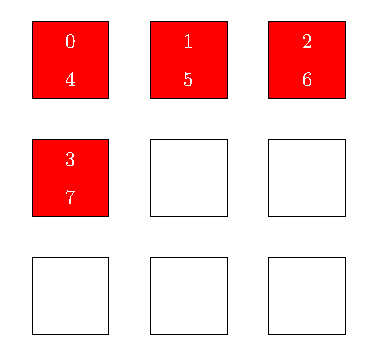
\includegraphics[width=0.4\textwidth]{figures/tikz/indexing/roundrobin.pdf}
\caption{Round-Robin Indexing of 8 MPI Ranks on 4 Compute Nodes}
\label{fig:indexing:round_robin}
\end{figure}
Finally, one may also choose

\begin{ViFile}
app1.launch_indexing = random
\end{ViFile}
Random allocation with random indexing is somewhat redundant.  
Random allocation with block indexing is \emph{not} similar to Cartesian allocation with random indexing.
Random indexing on a Cartesian allocation still gives a contiguous block of nodes,
even if consecutive MPI ranks are scattered around.
A random allocation (unless allocating the whole machine) will not give a contiguous set of nodes.

%% !TEX root = manual.tex

%\section{Configuring MPI}
%\label{sec:tutorial:mpi}
%
%The actual implementation of MPI collectives and even the underlying protocol of MPI send/recv operations is highly configurable.
%Here we introduce the MPI tuning parameters and what they mean for performance experiments.
%
%\subsection{MPI Implementation}
%\label{subsec:mpi:implementation}
%
%The MPI implementation itself is flexible to change depending on how you want to utilize the network hardware.
%The default parameter is \inlineshell{mpi_implementation = basic},
%which only uses basic eager and rendezvous protocols and does not use RDMA.
%The cutoff for eager to rendezvous can be tuned by specifying, e.g.
%
%\begin{ViFile}
%mpi_handshake_size = 8KB
%\end{ViFile}
%giving the cutoff as an arbitrary byte length.
%
%For more complicated protocols, we can specify \inlineshell{mpi_implementation = rdma},
%which now allows a fancier set of protocols that leverage RDMA.
%The parameters here are tuned, e.g.
%
%\begin{ViFile}
%smp_single_copy_size = 8KB
%max_eager_msg_size = 8KB
%max_vshort_msg_size = 1KB
%\end{ViFile}
%
%The details of these protocols are best explained in the presentation ``Tuning the MPI Runtime Environment and Best Practices for Message Passing on Hopper''
%at \url{https://www.nersc.gov/assets/NUG-Meetings/2012/HowardP-MPI-NUG2012.png}.
%The parameter \inlineshell{smp_single_copy_size} is for intranode message passing.
%For small messages below the cutoff, an eager protocol is used where the message is copied into an intermediate buffer.
%For larger messages wishing to have zero-copy, a rendezvous protocol is used and the message is directly copied from send to receive buffer.
%The parameter \inlineshell{max_eager_msg_size} controls the crossover from an eager protocol using send buffers to a rendezvous protocol with zero-copy.
%Both the eager and rendezvous protocol use RDMA, creating a bit of a latency overhead.
%For very small messages, a special pathway can be taken avoiding RDMA and just directly sending the small message into a pre-allocated mailbox on the receiver.
%The cutoff for very small messages is given by \inlineshell{max_vshort_msg_size}.
%
%\subsection{MPI Collectives}
%The implementation of individual collectives can vary widely depending on the platform, message size, or distribution.
%\sstmacro provides limited flexibility for tuning collectives, but infrastructure is being developed to allow very fine-grained tuning
%of which MPI collective algorithms are used.  Currently, only MPI\_Allgather and MPI\_Allreduce can have alternative implementations chosen.
%For MPI\_Allgather, in the input file, one can specify \inlineshell{mpi_allgather = ring} or \inlineshell{mpi_allgather = bruck}
%to use either a basic ring algorithm or to use the Br{\"u}ck algorithm.  In the same way, one can either specify
%\inlineshell{mpi_allgather = rabenseifner} or \inlineshell{mpi_allgather = wilke}.
%More details can be found in ``Optimization of Collective Communication Operations in MPICH'' by Rajeev Thakur and Rolf Rabenseifner.
%The Wilke algorithm is a variation binary blocks algorithm described therein.
%Future versions of \sstmacro are expected to include a more complete library of collective algorithms with the ability to tune which algorithms are selected for specific buffer sizes.
%
%\subsection{MPI Queue}
%The implementation of the progress engine in MPI can either be a service (asynchronous progress thread distinct from the application) or an integrated part of the application.
%Most current MPI implementations have integrated progress engines that only move forward inside MPI\_Wait or MPI\_Test calls.
%However, you may wish to experiment with what performance gains can be had with an asynchronous progress thread.
%For the parameter \inlineshell{mpi_queue_thread_type}, you can either specify \inlineshell{user}, integrated progress engine that is part of the user application,
%or \inlineshell{service}, progress engine on asynchronous thread.
%If using the call graph feature (Section \ref{sec:tutorials:callgraph}), far more detail is available if using the integrated engine with \inlineshell{user}.

%% !TEX root = manual.tex

\section{Discrete Event Simulation}
\label{sec:tutorial:des}
Although not necessary for using the simulator, a basic understanding of discrete event simulation can be helpful in giving users an intuition for network models and parameters.
Here we walk through a basic program that executes a single send/recv pair.
\sstmacro simulates many parallel processes, but itself runs as a single process with only one address space (\sstmacro can actually run in parallel mode, but we ignore that complication here).
\sstmacro manages each parallel process as a user-space thread (application thread), allocating a thread stack and frame of execution.
User-space threading is necessary for large simulations since otherwise the kernel would be overwhelmed scheduling thousands of threads.

\sstmacro is driven by a simulation thread which manages the user-space thread scheduling (Figure \ref{fig:des}).
In the most common (and simplest) use case, all user-space threads are serialized, running one at a time.
The main simulation thread must manage all synchronizations, yielding execution to process threads at the appropriate times.
The main simulation thread is usually abbreviated as the DES (discrete event simulation) thread.
The simulation progresses by scheduling future events.  
For example, if a message is estimated to take 5 $\mu$s to arrive,
the simulator will schedule a MESSAGE ARRIVED event 5 $\mu$s ahead of the current time stamp.
Every simulation starts by scheduling the same set of events: launch process 0, launch process 1, etc.

\begin{figure}[h!]
\centering
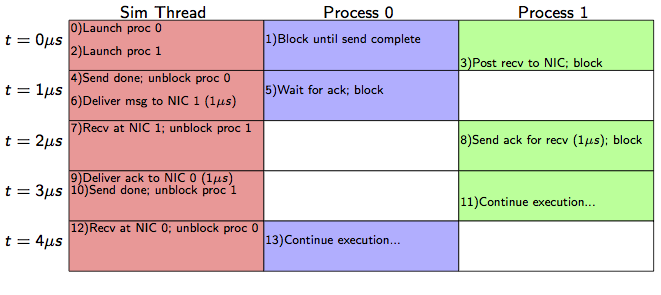
\includegraphics[width=0.95\textwidth]{figures/tikz/des/events.png}
\caption{Progression of Discrete Event Simulation for Simple Send/Recv Example}
\label{fig:des}
\end{figure}

The simulation begins at time $t=0\mu s$.  
The simulation thread runs the first event, launching process 0.
The context of process 0 is switched in, and \sstmacro proceeds running code as if it were actually process 0.
Process 0 starts a blocking send in Event 1.
For process 0 to perform a send in the simulator, it must \emph{schedule} the necessary events to simulate the send.
Most users of \sstmacro will never need to explicitly schedule events.
Discrete event details are always hidden by the API and executed inside library functions.
In this simple case, the simulator estimates the blocking send will take 1 $\mu$s.
It therefore schedules a SEND DONE (Event 4) 1 $\mu$s into the future before blocking.
When process 0 blocks, it yields execution back to the main simulation.

At this point, no time has yet progressed in the simulator.
The DES thread runs the next event, launching process 1, which executes a blocking receive (Event 3).
Unlike the blocking send case, the blocking receive does not schedule any events.
It cannot know when the message will arrive and therefore blocks without scheduling a RECV DONE event.
Process 1 just registers the receive and yields back to the DES thread.

At this point, the simulator has no events left at t=0 $\mu$s and so it must progress its time stamp.
The next event (Event 4) is SEND DONE at t=1 $\mu$s. The event does two things.
First, now that the message has been injected into the network, the simulator estimates when it will arrive at the NIC of process 1.
In this case, it estimates 1 $\mu$s and therefore schedules a MESSAGE ARRIVED event in the future at t=2 $\mu$s (Event 7).
Second, the DES thread unblocks process 0, resuming execution of its thread context.
Process 0 now posts a blocking receive, waiting for process 1 to acknowledge receipt of its message.

The simulator is now out of events at t=1 $\mu$s and therefore progresses its time stamp to t=2 $\mu$s.
The message arrives (Event 7), allowing process 1 to complete its receive and unblock.
The DES thread yields execution back to process 1, which now executes a blocking send to ack receipt of the message.
It therefore schedules a SEND DONE event 1 $\mu$s in the future (Event 10) and blocks, yielding back to the DES thread.
This flow of events continues until all the application threads have terminated.
The DES thread will run out of events, bringing the simulation to an end. 



%% !TEX root = manual.tex

\section{Using DUMPI}
\label{sec:tutorial:dumpi}

\subsection{Building DUMPI}
\label{subset:dump:build}
As noted in the introduction, \sstmacro is primarily intended to be an on-line simulator. Real application code runs, but \sstmacro  intercepts calls to communication (MPI) and computation functions to simulate time passing.  However, \sstmacro can also run off-line, replaying application traces collected from real production runs.  This trace collection and trace replay library is called DUMPI.

Although DUMPI is automatically included as a subproject in the \sstmacro download, trace collection can be easier if DUMPI is built independently from \sstmacro.  The code can be downloaded from \url{https://bitbucket.org/sst-ca/dumpi}. If downloaded through Mercurial, one must initialize the build system and create the configure script.

\begin{ShellCmd}
dumpi$ ./bootstraps.h
\end{ShellCmd}

DUMPI must be built with an MPI compiler.

\begin{ShellCmd}
dumpi/build$ ../configure CC=mpicc CXX=mpicxx \ 
	              --enable-libdumpi --prefix=$DUMPI_PATH
\end{ShellCmd}
The \inlineshell{--enable-libdumpi} flag is needed to configure the trace collection library.
After compiling and installing, a \inlineshell{libdumpi.\$prefix} will be added to \inlineshell{\$DUMPI_PATH/lib}.

Collecting application traces requires only a trivial modification to the standard MPI build.
Using the same compiler, simply add the DUMPI library path and library name to your project's \inlineshell{LDFLAGS}.

\begin{ShellCmd}
your_project/build$ ../configure CC=mpicc CXX=mpicxx \
                                  LDFLAGS=``-L$DUMPI_PATH/lib -ldumpi"
\end{ShellCmd}

\subsubsection{Trace Collection}
\label{subsec:dumpi:tracecollection}
DUMPI works by overriding \emph{weak symbols} in the MPI library.
In all MPI libraries, functions such as \inlinecode{MPI_Send} are only weak symbol wrappers to the actual function \inlinecode{PMPI_Send}.
DUMPI overrides the weak symbols by implementing functions with the symbol \inlinecode{MPI_Send}. 
If a linker encounters a weak symbol and regular symbol with the same name, it ignores the weak symbol.
DUMPI functions look like

\begin{CppCode}
int MPI_Send(...)
{
	/** Start profiling work */
	...
	int rc = PMPI_Send(...);
	/** Finish profiling work */
	...
	return rc;
}
\end{CppCode}
collecting profile information and then directly calling the PMPI functions.

We examine DUMPI using a very basic example program.

\begin{CppCode}
#include <mpi.h>
int main(int argc, char** argv)
{
    MPI_Init(&argc, &argv);
    MPI_Finalize();
    return 0;
}
\end{CppCode}
After compiling the program named \inlineshell{test} with DUMPI, we run MPI in the standard way.

\begin{ShellCmd}
example$ mpiexec -n 2 ./test
\end{ShellCmd}
After running, there are now three new files in the directory.

\begin{ShellCmd}
example$ ls dumpi*
dumpi-2013.09.26.10.55.53-0000.bin	
dumpi-2013.09.26.10.55.53-0001.bin	
dumpi-2013.09.26.10.55.53.meta
\end{ShellCmd}
DUMPI automatically assigns a unique name to the files from a timestamp.
The first two files are the DUMPI binary files storing separate traces for MPI rank 0 and rank 1.
The contents of the binary files can be displayed in human-readable form by running the \inlineshell{dumpi2ascii}
program, which should have been installed in \inlineshell{\$DUMPI_PATH/bin}.

\begin{ShellCmd}
example$ dumpi2ascii dumpi-2013.09.26.10.55.53-0000.bin
\end{ShellCmd}
This produces the output

\begin{ViFile}
MPI_Init entering at walltime 8153.0493, cputime 0.0044 seconds in thread 0.
MPI_Init returning at walltime 8153.0493, cputime 0.0044 seconds in thread 0.
MPI_Finalize entering at walltime 8153.0493, cputime 0.0045 seconds in thread 0.
MPI_Finalize returning at walltime 8153.0498, cputime 0.0049 seconds in thread 0.
\end{ViFile}

The third file is just a small metadata file DUMPI used to configure trace replay.
\begin{ViFile}
hostname=deepthought.magrathea.gov
numprocs=2
username=slartibartfast
startime=1380218153
fileprefix=dumpi-2013.09.26.10.55.53
version=1
subversion=1
subsubversion=0
\end{ViFile}

\subsubsection{Trace Replay}
\label{subsec:dumpi:tracereplay}
It is often useful to validate the correctness of a trace.  Sometimes there can be problems with trace collection. 
There are also a few nooks and crannies of the MPI standard left unimplemented.
To validate the trace, you can run in a special debug mode that runs the simulation with a very coarse-grained model
to ensure as quickly as possible that all functions execute correctly.
This can be done straightforwardly by running the executable with the dumpi flag: \inlineshell{sstmac --dumpi}.

To replay a trace in the simulator, a small modification is required to the example input file in \ref{sec:parameters}.
We have two choices for the trace replay.  First, we can attempt to \emph{exactly} replay the trace as it ran on the host machine.
Second, we could replay the trace on a new machine or different layout.

For exact replay, the key issue is specifying the machine topology.
For some architectures, topology information can be directly encoded into the trace.
This is generally true on Blue Gene, but not Cray.
When topology information is recorded, trace replay is much easier.
The parameter file then becomes, e.g.

\begin{ViFile}
launch_app1_type = dumpi
launch_indexing = dumpi
launch_allocation = dumpi
launch_app1 = parsedumpi
launch_dumpi_metaname = testbgp.meta
\end{ViFile}
We have a new parameter \inlinefile{launch_app1_type} set to \inlinefile{dumpi}.
This was implicit before, taking the default value of \inlinefile{skeleton}.
We also set indexing and allocation parameters to read from the DUMPI trace.
The application name in \inlinefile{launch_app1} is a special app that parses the DUMPI trace.
Finally, we direct \sstmacro to the DUMPI metafile produced when the trace was collected.
To extract the topology information, locate the \inlineshell{.bin} file corresponding to MPI rank 0.
To print topology info, run

\begin{ShellCmd}
traces$ dumpi2ascii -H testbgp-0000.bin 
\end{ShellCmd}
which produces the output

\begin{ViFile}
version=1.1.0
starttime=Fri Nov 22 13:53:58 2013
hostname=R00-M1-N01-J01.challenger
username=<none>
meshdim=3
meshsize=[4, 2, 2]
meshcrd=[0, 0, 0]
\end{ViFile}
Here we see that the topology is 3D with extent 4,2,2 in the X,Y,Z directions.
At present, the user must still specify the topology in the parameter file.
Even though \sstmacro can read the topology \emph{dimensions} from the trace file,
it cannot read the topology \emph{type}.  It could be a torus, dragonfly, or fat tree.
The parameter file therefore needs

\begin{ViFile}
topology_name = hdtorus
topology_geometry = 4 2 2
\end{ViFile}
Beyond the topology, the user must also specify the machine model with bandwidth and latency parameters.
Again, this is information that cannot be automatically encoded in the trace.
It must be determined via small benchmarks like ping-pong.
An example file can be found in the test suite in \inlineshell{tests/test_configs/testdumpibgp.ini}.

If no topology info could be recorded in the trace, more work is needed.
The only information recorded in the trace is the hostname of each MPI rank.
The parameters are almost the same, but with allocation now set to \inlinefile{hostname}.
Since no topology info is contained in the trace, 
a hostname map must be put into a text file that maps a hostname to the topology coordinates.
The new parameter file, for a fictional machine called deep thought

\begin{ViFile}
# Launch parameters
launch_app1_type = dumpi
launch_indexing = dumpi
launch_allocation = hostname
launch_app1 = parsedumpi
launch_dumpi_metaname = dumpi-2013.09.26.10.55.53.meta
launch_dumpi_mapname = deepthought.map
# Machine parameters
topology_name = torus
topology_geometry = 2 2
\end{ViFile}


In this case, we assume a 2D torus with four nodes.
Again, DUMPI records the hostname of each MPI rank during trace collection.
In order to replay the trace, the mapping of hostname to coordinates must be given in a node map file,
specified by the parameter \inlinefile{launch_dumpi_mapname}.
The node map file has the format

\begin{ViFile}
4 2
nid0 0 0
nid1 0 1
nid2 1 0
nid3 1 1
\end{ViFile}
where the first line gives the number of nodes and number of coordinates, respectively.
Each hostname and its topology coordinates must then be specified.
More details on building hostname maps are given below.

We can also use the trace to experiment with new topologies to see performance changes.
Suppose we want to test a crossbar topology.

\begin{ViFile}
# Launch parameters
launch_indexing = block
launch_allocation = first_available
launch_app1 = parsedumpi
launch_app1_size = 2
launch_dumpi_metaname = dumpi-2013.09.26.10.55.53.meta
# Machine parameters
topology_name = crossbar
topology_geometry = 4
\end{ViFile}
We no longer use the DUMPI allocation and indexing. 
We also no longer require a hostname map.
The trace is only used to generate MPI events and no topology or hostname data is used.
The MPI ranks are mapped to physical nodes entirely independent of the trace.

\subsubsection{Building the Hostname Map}
\label{subsec:dumpi:hostnamemap} 
Not all HPC machines support topology queries.  
The current scheme is only valid for Cray machines, which support topology queries via \inlineshell{xtdb2proc}.
NOTE: As of 01/15/2014, this command seems to be broken at NERSC.
\sstmacro comes with a script in the bin folder, \inlineshell{xt2nodemap.pl}, that parses the Cray file
into the DUMPI format.  We first run

\begin{ShellCmd}
cray$ xtdb2proc -f - > db.txt
\end{ShellCmd}
to generate a Cray-formatted file \inlineshell{db.txt}.
Next we run the conversion script

\begin{ShellCmd}
cray$ xt2nodemap.pl -t hdtorus < db.txt > nodemap.txt
\end{ShellCmd}
generating the hostname map.

%% !TEX root = manual.tex

\section{Using Score-P and OTF2 (Beta)}
\label{sec:tutorial:otf}

OTF2 is part of Score-P. Sources for both can be found here 
\begin{ViFile}
http://www.vi-hps.org/projects/score-p
\end{ViFile}


Trace collection requires both Score-P and OTF2 installations. Trace replay with SST/macro requires OTF2.


\subsection{Trace Collection}
\label{subsec:otf:traceCollection}
Score-P's default collection strategy will include every function call in the trace, making even small programs produce untenably large traces. Score-P supports collection filters, which can restrict collection at a minimum to MPI and OMP function calls. At the end of the program's runtime, traces from each rank are put in a common directory.  An MPI program must be compiled with Score-P to produce traces:

\begin{ShellCmd}
scorep-mpicxx -o test.exe test.cc
\end{ShellCmd}



To limit the size of the traces, run the program with:

\begin{ViFile}
# these environment variables are picked up by Score-P at runtime
export SCOREP_ENABLE_TRACING=true
export SCOREP_TOTAL_MEMORY=1G
export SCOREP_FILTERING_FILE='scorep.filter'

mpirun -n 2 test.exe
\end{ViFile}

The file \inlineshell{scorep.filter} should contain:
\begin{ViFile}
SCOREP_REGION_NAMES_BEGIN EXCLUDE *
\end{ViFile}


To view a plain-text representation of the trace after running, use the otf2-print tool.

\begin{ViFile}
otf2-print scorep-*/traces.otf2
\end{ViFile}

\subsection{Trace Replay}
\label{subsec:otf:traceReplay}
SST/macro will use a trace replay skeleton for OTF2 in much the same way as it does for dumpi. SST/macro trace replays configured using *.ini files. 

\begin{ViFile}
...

node {
 app1 {
  otf2_timescale = 1.0
  name = otf2_trace_replay_app
  size = N
  otf2_metafile = <trace-root>/scorep-20170309_1421_27095992608015568/traces.otf2
 # debugging output
  otf2_print_mpi_calls=false
  otf2_print_trace_events=false
  otf2_print_time_deltas=false
  otf2_warn_unknown_callback=false
 }
}

\end{ViFile}

%% !TEX root = manual.tex

\section{Outputing Statistics}


%% !TEX root = manual.tex

\section{OTF2 Trace Creation}
\label{sec:otf:traceEmission}
SST/macro can emmit OTF2 traces from MPI simulations. This gets activated by:

\begin{ViFile}
...

node {
 app1 {
  ...
    otf2 {
      fileroot = dump
    }
  ...
 }
}

\end{ViFile}



%% !TEX root = manual.tex

\section{Call Graph Visualization}
\label{sec:tutorials:callgraph}
Generating call graphs requires a special build of \sstmacro.

\begin{ShellCmd}
build> ../configure --prefix=$INSTALL_PATH --enable-graphviz
\end{ShellCmd}
The \inlineshell{--enable-graphviz} flag defines an instrumentation macro throughout the \sstmacro code.
This instrumentation must be \emph{compiled} into \sstmacro.
In the default build, the instrumentation is not added since the instrumentation has a high overhead.
However, \sstmacro only instruments a select group of the most important functions so the overhead should only be 10-50\%.
After installing the instrumented version of \sstmacro, a call graph must be activated as part of the OS component.

\begin{ViFile}
node {
  os {
    callGraph {
      fileroot = <fileroot>
    }
  }
}
\end{ViFile}
After running, a \inlineshell{<fileroot>.callgrind.out} file should appear in the folder.

To visualize the call graph, you must download KCachegrind: \url{http://kcachegrind.sourceforge.net/html/Download.html}.
KCachegrind is built on the KDE environment, which is simple to build for Linux but can be very tedious for Mac.
The download also includes a QCachegrind subfolder, providing the same functionality built on top of Qt.  
This is highly recommended for Mac users.

\begin{figure}[h]
\centering
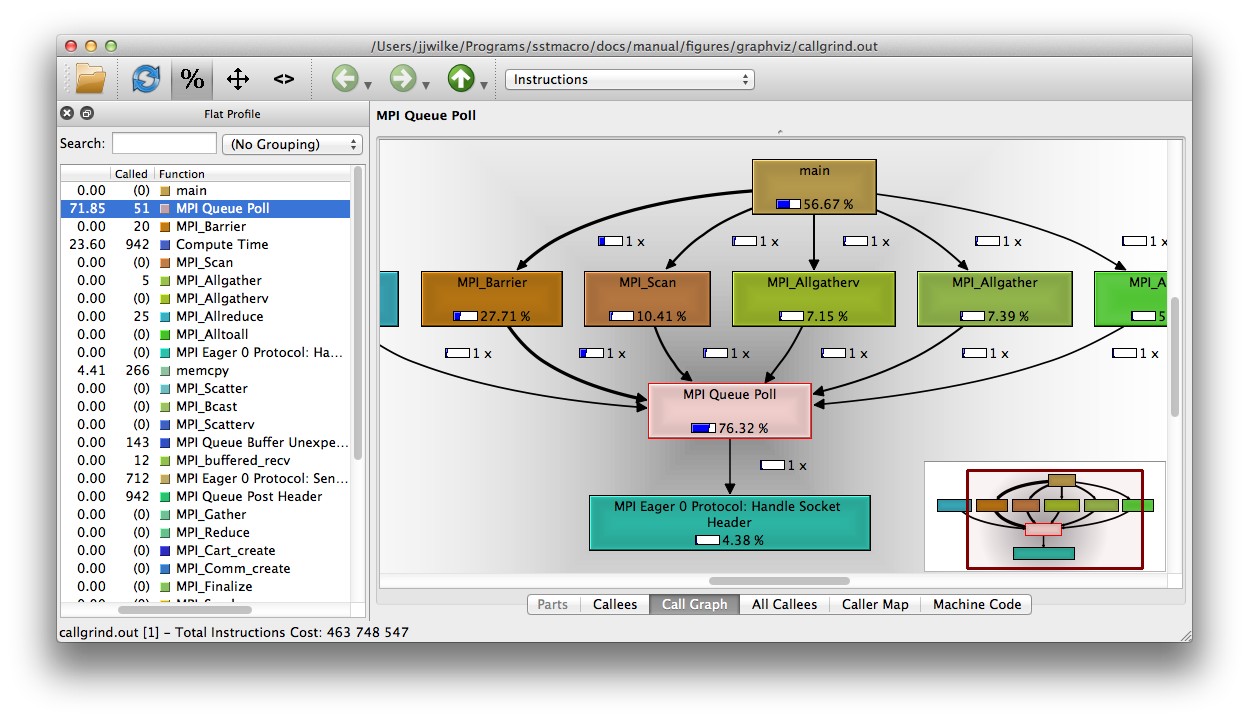
\includegraphics[width=0.95\textwidth]{figures/graphviz/gui.png}
\caption{QCachegrind GUI}
\label{fig:qcgui}
\end{figure}

The basic QCachegrind GUI is shown in Figure \ref{fig:qcgui}.  
On the left, a sidebar contains the list of all functions instrumented with the percent of total execution time spent in the function.
In the center pane, the call graph is shown.  
To navigate the call graph, a small window in the bottom right corner can be used to change the view pane.
Zooming into one region (Figure \ref{fig:qcgraphone}), we see a set of MPI functions (Barrier, Scan, Allgatherv).
Each of the functions enters a polling loop, which dominates the total execution time.  
A small portion of the polling loop calls the ``Handle Socket Header'' function.
Double-clicking this node unrolls more details in the call graph (Figure \ref{fig:qcgraphtwo}).
Here we see the function splits execution time between buffering messages (memcpy) and posting headers (Compute Time).

\begin{figure}[h!]
\centering
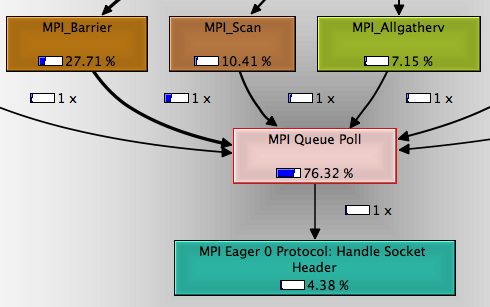
\includegraphics[width=0.55\textwidth]{figures/graphviz/callgraph1.png}
\caption{QCachegrind Call Graph of MPI Functions}
\label{fig:qcgraphone}
\end{figure}

\begin{figure}[h!]
\centering
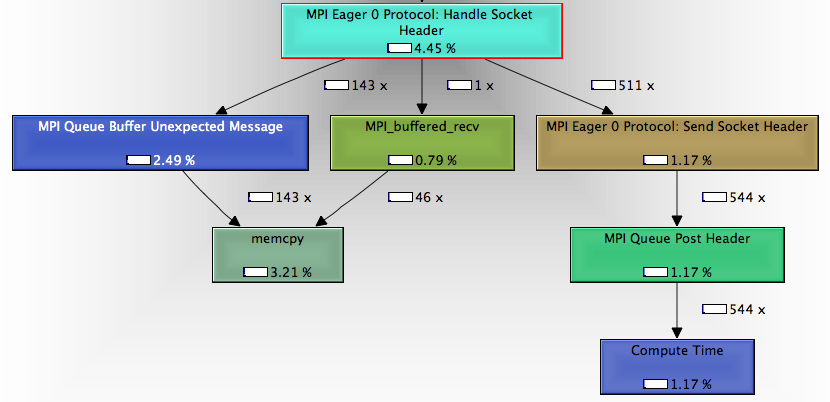
\includegraphics[width=0.75\textwidth]{figures/graphviz/callgraph2.png}
\caption{QCachegrind Expanded Call Graph of Eager 0 Function}
\label{fig:qcgraphtwo}
\end{figure}


%% !TEX root = manual.tex

\section{Spyplot Diagrams}
\label{sec:tutorials:spyplot}

Spyplots visualize communication matrices, showing either the number of messages or number of bytes sent between two network endpoints.
They are essentially contour diagrams, where instead of a continuous function $F(x,y)$ we are plotting the communication matrix $M(i,j)$.
An example spyplot is shown for a simple application that only executes an MPI\_Allreduce (Figure \ref{fig:spyplot}).
Larger amounts of data (red) are sent to nearest neighbors while decreasing amounts (blue) are sent to MPI ranks further away.

\begin{figure}[h]
\centering
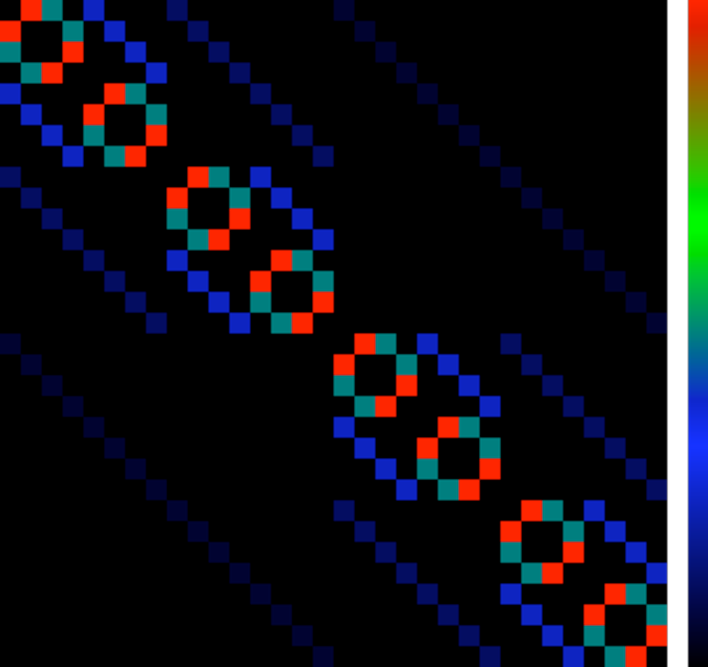
\includegraphics[width=0.4\textwidth]{figures/spyplot/mpi_spyplot.pdf}
\caption{Spyplot of Bytes Transferred Between MPI Ranks for MPI\_Allreduce}
\label{fig:spyplot}
\end{figure}

Various spyplots can be activated by boolean parameters in the input file.
The most commonly used are the MPI spyplots, for which you must add

\begin{ViFile}
mpi_spyplot = <fileroot>
\end{ViFile}

After running there will be a .csv and .png file in the folder, with e.g. \inlineshell{fileroot = test}

\begin{ShellCmd}
example> ls 
test.png
test.csv
\end{ShellCmd}
\inlineshell{test.png} shows the number of bytes exchanged between MPI ranks.
To extend the analysis you can specify

\begin{ViFile}
network_spyplot = <fileroot>
\end{ViFile}
A new csv/png will appear showing the number of bytes exchanged between physical nodes, 
accumulating together all MPI ranks sharing the same node.
This gives a better sense of spatial locality when many MPI ranks are on the same node.




%% !TEX root = manual.tex

\begin{figure}[h!]
\centering
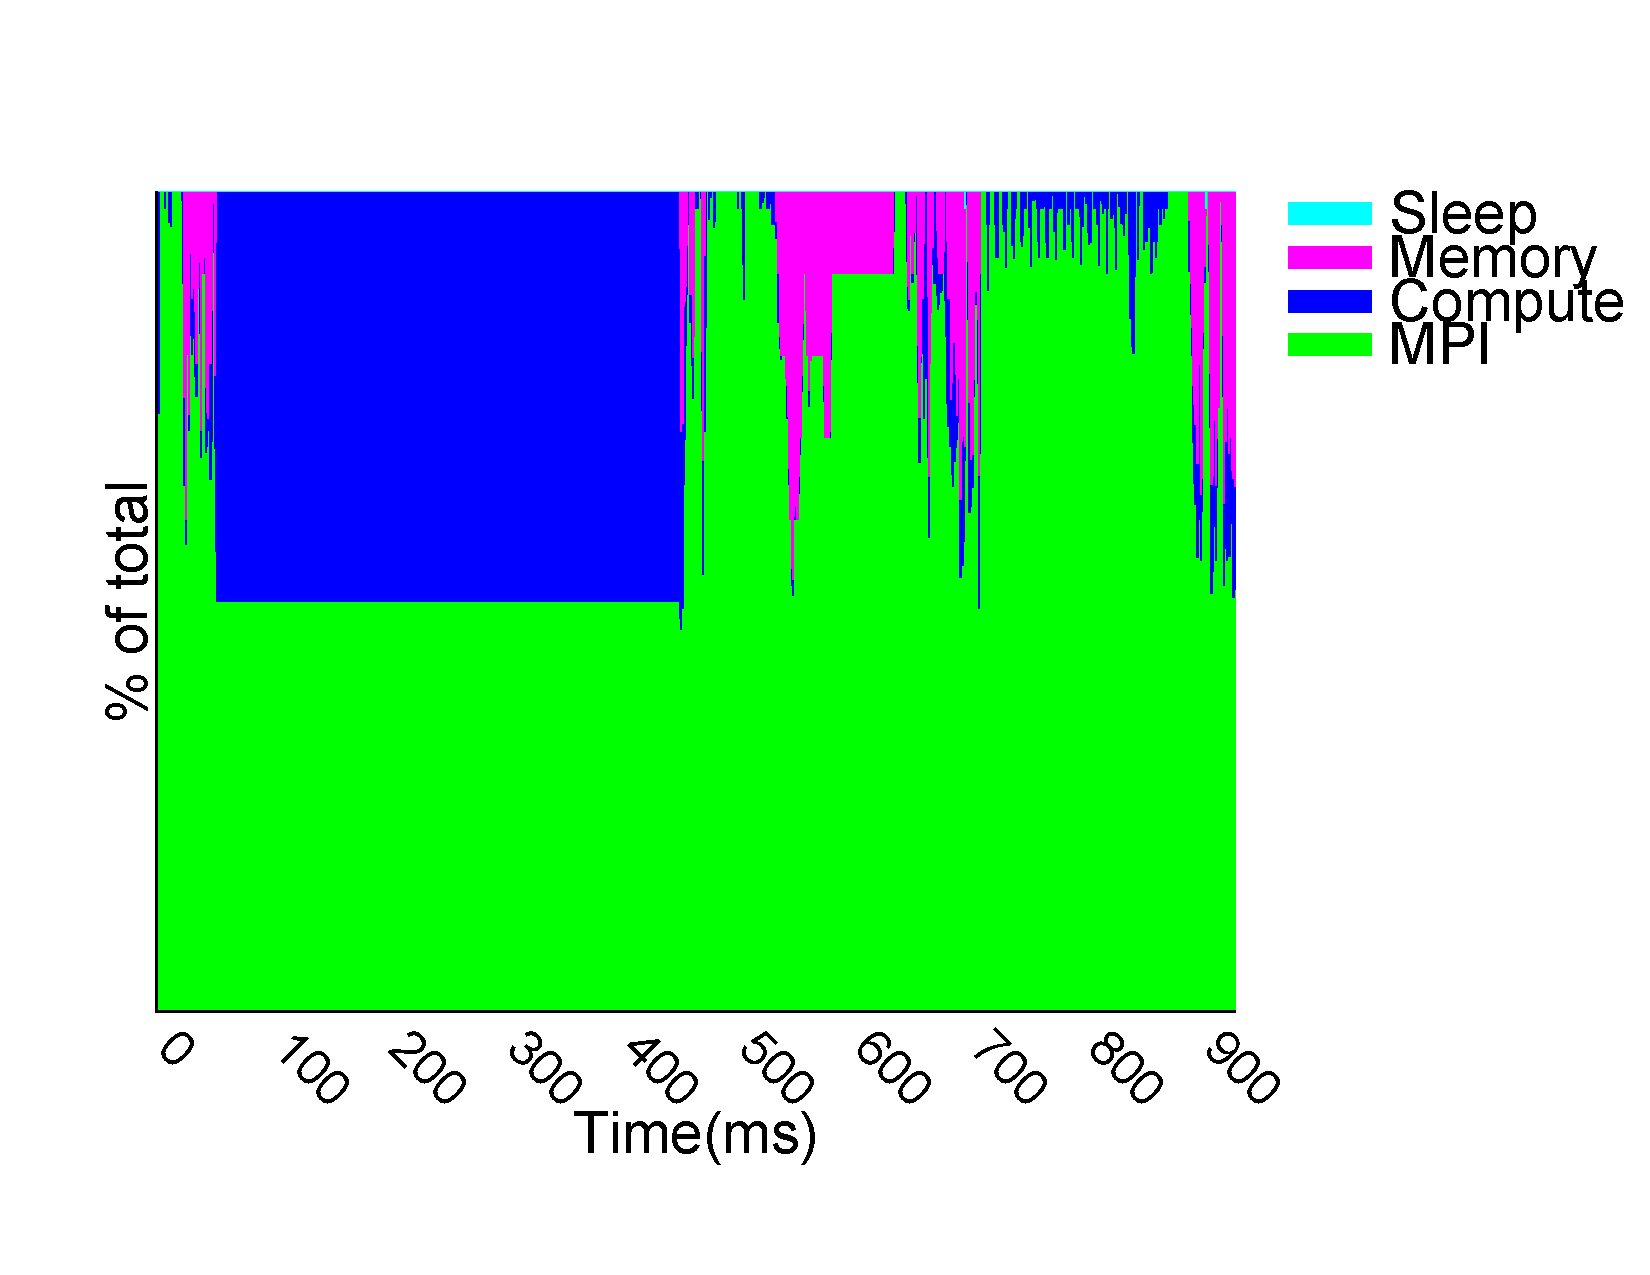
\includegraphics[width=0.6\textwidth]{figures/gnuplot/ftq/ftq.pdf}
\caption{Application Activity (Fixed-Time Quanta; FTQ) for Simple MPI Test Suite}
\label{fig:ftq}
\end{figure}
\section{Fixed-Time Quanta Charts}
\label{sec:tutorials:ftq}
Another way of visualizing application activity is a fixed-time quanta (FTQ) chart.
While the call graph gives a very detailed profile of what code regions are most important for the application, they lack temporal information.
The FTQ histogram gives a time-dependent profile of what the application is doing (Figure \ref{fig:ftq}).
This can be useful for observing the ratio of communication to computation.
It can also give a sense of how ``steady'' the application is, 
i.e. if the application oscillates between heavy computation and heavy communication or if it keeps a constant ratio.
In the simple example, Figure \ref{fig:ftq}, we show the FTQ profile of a simple MPI test suite with random computation mixed in.
In general, communication (MPI) dominates.  However, there are a few compute-intensive and memory-intensive regions.

The FTQ visualization is activated by another input parameter

\begin{ViFile}
ftq = <fileroot>
\end{ViFile}

where the \inlinefile{fileroot} parameter gives a unique prefix for the output files. 

After running, two new files appear in the folder: \inlineshell{<fileroot>_app1.p} and \inlineshell{<fileroot>_app1.dat}.
\inlineshell{plot_app1.p} is a Gnuplot script that generates the histogram as a postscript file.

\begin{ShellCmd}
your_project$ gnuplot plot_app1.p > output.ps
\end{ShellCmd}
Gnuplot can be downloaded from \url{http://www.gnuplot.info} or installed via MacPorts.
We recommend version 4.4, but at least 4.2 should be compatible.

The granularity of the chart is controlled by the \inlinefile{ftq_epoch} parameter in the input file. 
The above figure was collected with

\begin{ViFile}
ftq_epoch=5us
\end{ViFile}
Events are accumulated into a single data point per ``epoch.''
If the timestamp is too small, too little data will be collected and the time interval won't be large enough to give a meaningful picture.
If the timestamp is too large, too many events will be grouped togther into a single data point, losing temporal structure.


%% !TEX root = manual.tex

\section{Network Packet Statistics}
\label{sec:tutorials:packetStats}





%% !TEX root = manual.tex

\chapter{Topologies}
\label{chapter:topologies}

The torus topology is straightforward and easy to understand.
Here we introduce the basics of other topologies within SST that are more complex and require extra documentation to configure properly.
These are generally higher-radix or path-diverse topologies like fat tree, dragonfly, and flattened butterfly.
As noted in \ref{sec:tutorial:topology}, a more thorough and excellent discussions of these topologies is given in ``High Performance Datacenter Networks'' by Dennis Abts and John Kim.

%\section{Topology Query Utility}
%\label{sec:topologyQuery}
%Understanding topology inputs and geometries can sometimes be challenging.
%\sstmacro provides an executable for testing topology inputs and doing example coordinate computations.
%After making and installing, an executable \inlineshell{sstmac_top_info} will appear in the \inlineshell{bin} folder.
%The invocation of \inlineshell{sstmac_top_info} is exactly the same as the main \inlineshell{sstmac} executable.
%For the example parameter file named \inlineshell{machine.ini}:
%
%\begin{ViFile}
%topology.name = fat_tree
%topology.geometry = 4 3
%\end{ViFile}
%
%we run
%
%\begin{ShellCmd}
%bin> sstmac_top_info -f machine.ini
%\end{ShellCmd}
%which produces the output
%
%\begin{ViFile}
%Number of nodes:         81
%Number of leaf switches: 27
%Number of switches:      94
%\end{ViFile}
%
%detailing the produced geometry.  Here the fat tree has a total of 94 switches, 27 of which are ``leaf'' switches directly connected to compute nodes.
%The output is followed by the prompt
%
%\begin{ShellCmd}
%NextInput: 
%\end{ShellCmd}
%
%One can either enter a single number (switch ID) or set of coordinates.
%If given a switch ID, the coordinates are computed.
%If coordinates are given, the switch ID is computed.
%
%\begin{ShellCmd}
%NextInput: 32
%Switch ID maps to coordinates [ 2 0 1 2 ]
%NextInput: 2 0 1 2
%Coordinates map to switch ID 32
%\end{ShellCmd}
%
%The program is just exited with Ctrl-C.
%The meaning of the above coordinates is detail below for fat tree (Section \ref{sec:tutorial:fattree}).


% !TEX root = manual.tex
\section{Torus}
\label{subsec:tutorial:hypercube}

The torus is the simplest topology and fairly easy to understand.
We have already discussed basic indexing and allocation as well as routing.
More complicated allocation schemes with greater fine-grained control can be used such as the
coordinate allocation scheme (see hypercube below for examples) and the node ID allocation scheme (see fat tree below for examples).
More complicated Valiant and UGAL routing schemes are shown below for hypercube and dragonfly,
but apply equally well to torus.

For torus we illustrate here the Cartesian allocation for generating regular Cartesian subsets.
For this, the input file would look like 

\begin{ViFile}
topology.name = torus
topology.geometry = 4 4 4
app1.launch_cmd = aprun -n 8
app1.indexing = block
app1.allocation = cartesian
app1.cart_sizes = 2 2 2
app1.cart_offsets = 0 0 0
\end{ViFile}

This allocates a 3D torus of size 4x4x4.
Suppose we want to allocate all 8 MPI ranks in a single octant?
We can place them all in a 2x2x2 3D sub-torus by specifying the size of the sublock 
(\inlineshell{cart_sizes}) and which octant (\inlineshell{cart_offsets}).
This applies equally well to higher dimensional analogs.
This is particularly useful for allocation on Blue Gene machines
which always maintain contiguous allocations on a subset of nodes.

This allocation is slightly more complicated if we have multiple nodes per switch.
Even though we have a 3D torus, 
we treat the geometry as a 4D coordinate space with the 4th dimension referring to nodes connected to the same switch, 
i.e. if two nodes have the 4D coordinates [1 2 3 0] and [1 2 3 1] they are both connected to the same switch.
Consider the example below:

\begin{ViFile}
topology.name = torus
topology.geometry = 4 4 4
topology.concentration = 2
app1.launch_cmd = aprun -n 8
app1.indexing = block
app1.allocation = cartesian
app1.cart_sizes = 2 2 1 2
app1.cart_offsets = 0 0 0 0
\end{ViFile}

We allocate a set of switches across an XY plane (2 in X, 2 in Y, 1 in Z for a single plane).
The last entry in \inlineshell{cart_sizes} indicates that both nodes on each switch should be used.



% !TEX root = manual.tex
\section{Hypercube}
\label{subsec:tutorial:hypercube}

Although never used at scale in a production system, the generalized hypercube is an important topology to understand, particularly for flattened butterfly and dragonfly.
The (k,n) generalized hypercube is geometrically an N-dimensional torus with each dimension having size k (although dimension sizes need not be equal).
Here we show a (4,2) generalized hypercube (Figure \ref{fig:topologies:hypercubeConnected}).  This would be specified in SST as:

\begin{ViFile}
topology_name = hypercube
topology_geometry = 4 4 
\end{ViFile}
indicating size 4 in two dimensions. 

While a torus only has nearest-neighbor connections, a hypercube has full connectivity within a row and column (Figure \ref{fig:topologies:hypercubeConnected}).
Any switches in the same row or same column can send packets with only a single hop.

\begin{figure}[h!]
\centering
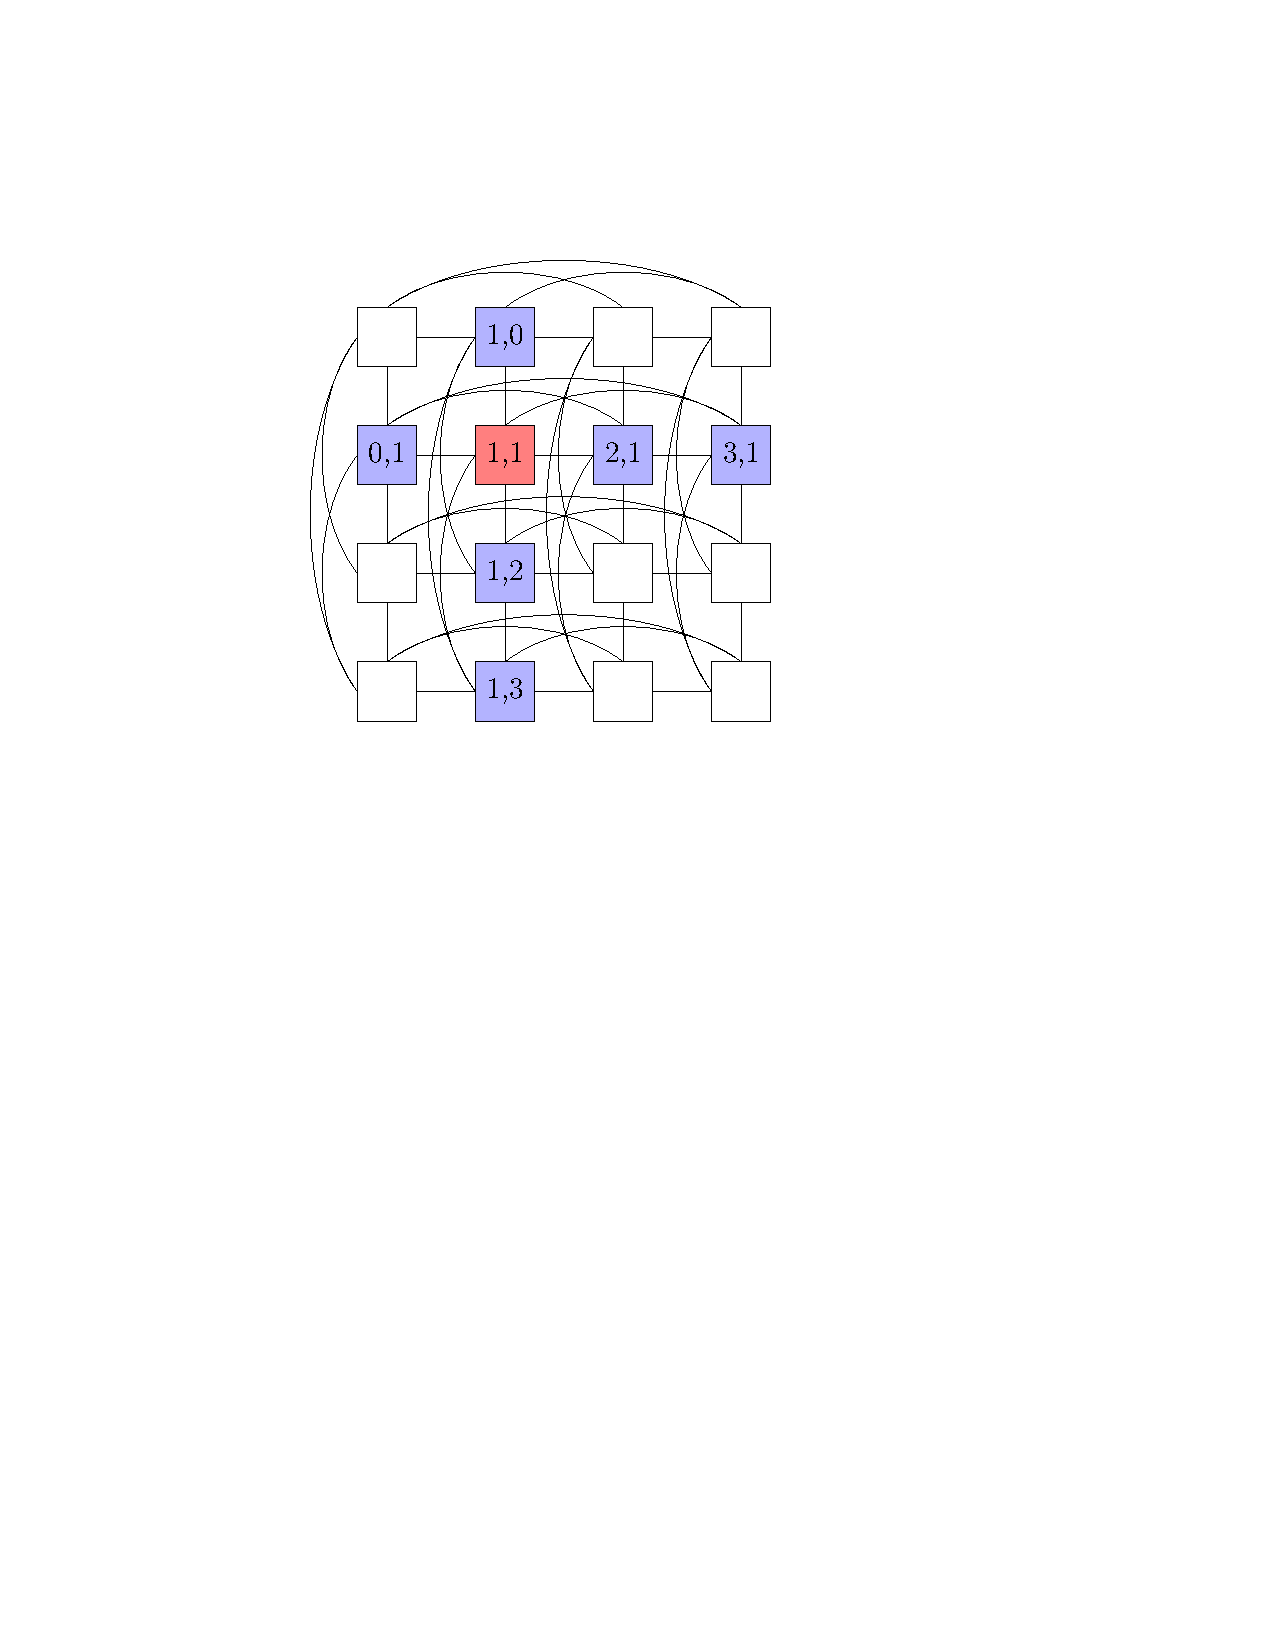
\includegraphics[width=0.5\textwidth]{figures/tikz/hypercube/hypercube_connected.pdf}
\caption{Hypercube with links and connections within a row/column}
\label{fig:topologies:hypercubeConnected}
\end{figure}

This extra connectivity leads to greater path diversity and higher radix switches.
The cost tradeoff is that each link has lower bandwidth than a torus. 
Whereas a torus has a few fat links connecting switches, a hypercube has many thin links.
A hypercube can have more dimensions and be asymmetric, e.g.

\begin{ViFile}
topology_name = hypercube
topology_geometry = 4 5 6
\end{ViFile}

where now we have full connections within horizontal rows, horizontal columns, and vertical columns.
Here each switch has radix 12 (3 connections in X, 4 connections in Y, 5 connections in Z). 

\subsection{Allocation and indexing}
A hypercube has the same coordinate system as a torus. For example, to create a very specific, irregular allocation on a hyerpcube:

\begin{ViFile}
launch_app1_cmd = aprun -n 5
launch_indexing = coordinate
launch_allocation = coordinate
launch_coordinate_file = coords.txt
\end{ViFile}

and then a coordinate file named \inlineshell{coords.txt}
\begin{ViFile}
5 2
0 0
0 1
1 1
2 0
3 3
\end{ViFile}
The first line indicates 5 entries each with 2 coordinates.
Each line then defines where MPI ranks 0-4 will be placed

\begin{figure}[h!]
\centering
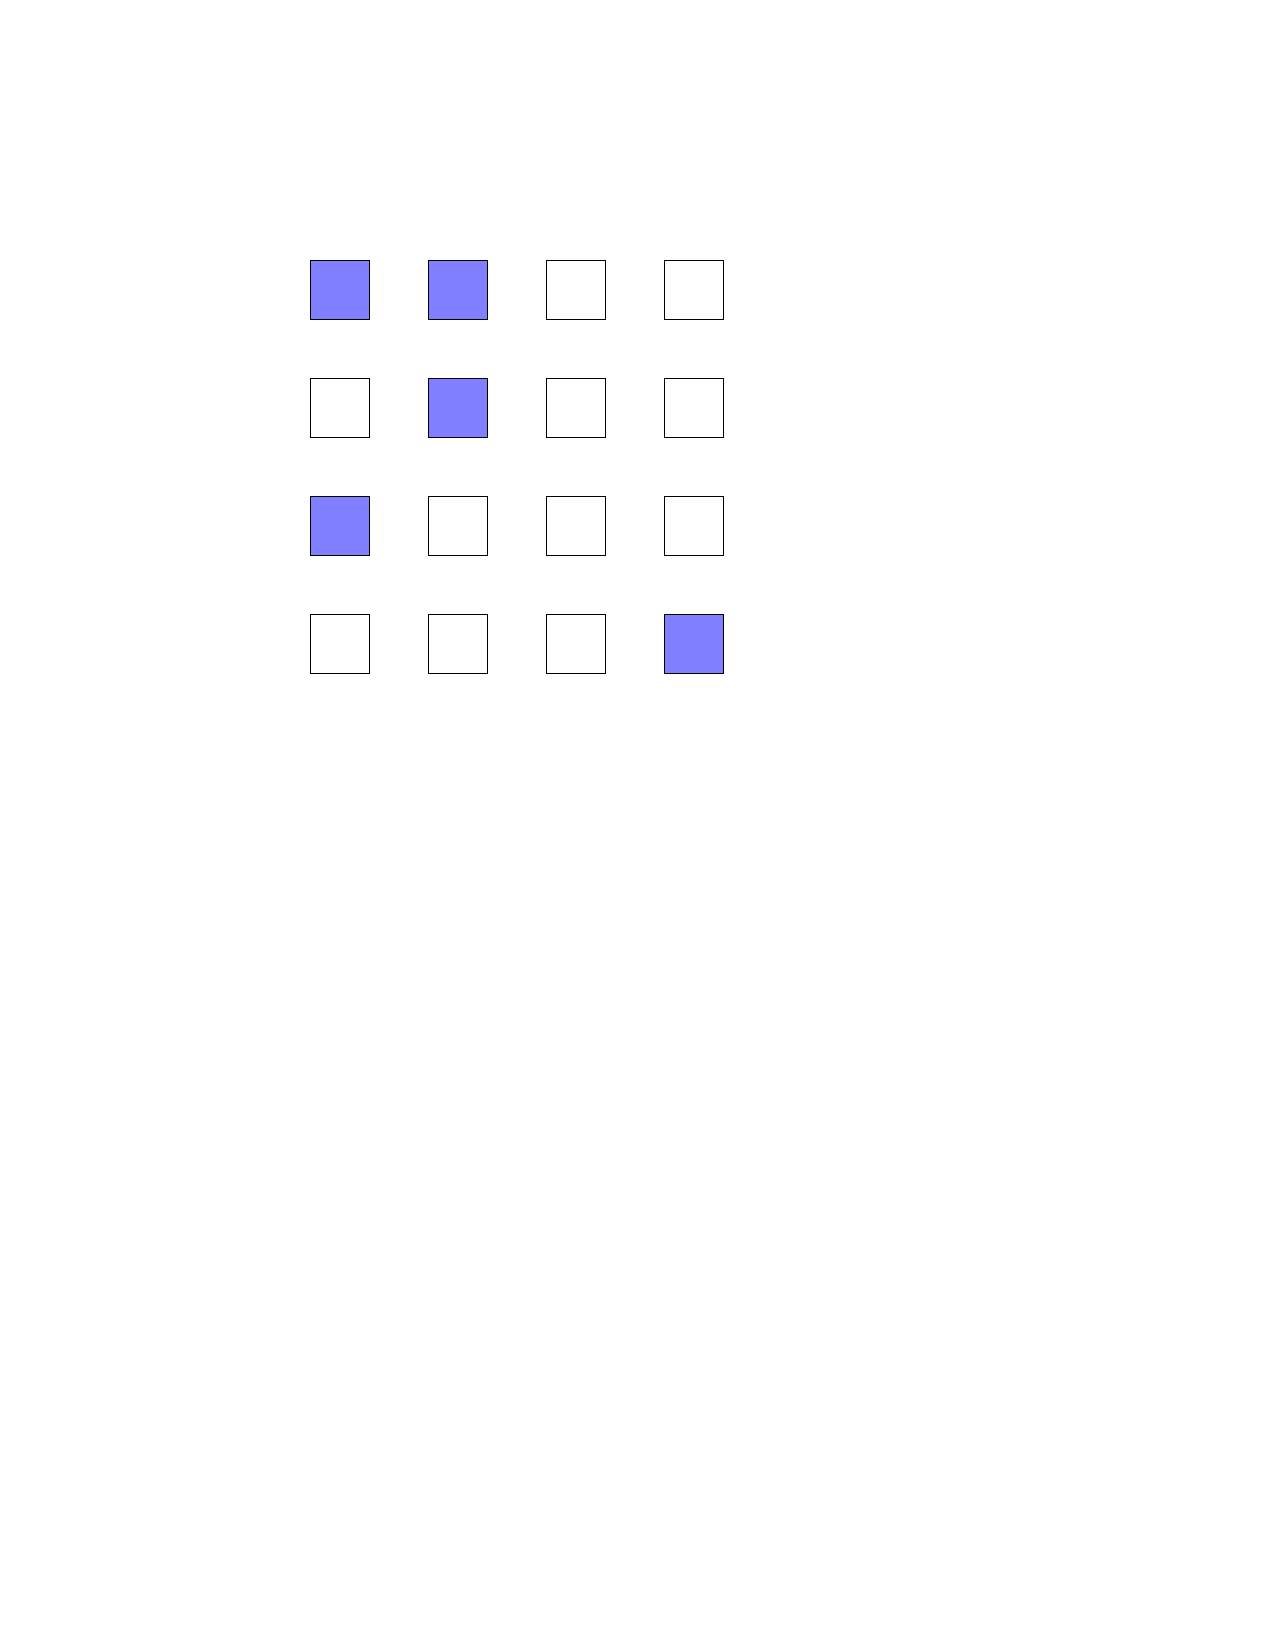
\includegraphics[width=0.5\textwidth]{figures/tikz/hypercube/hypercube_allocation.pdf}
\caption{Hypercube allocation for given set of coordinates}
\label{fig:topologies:hypercubeAllocation}
\end{figure}

\subsection{Routing}
Hypercubes allow very path-diverse routing because of its extra connections.
In the case of minimal routing (Figure \ref{fig:topologies:hypercubePath}), two different minimal paths from blue to red are shown.
While dimension order routing would rigorously go X then Y, you can still route minimally over two paths either randomly selecting to balance load or routing based on congestion.

\begin{figure}[h!]
\centering
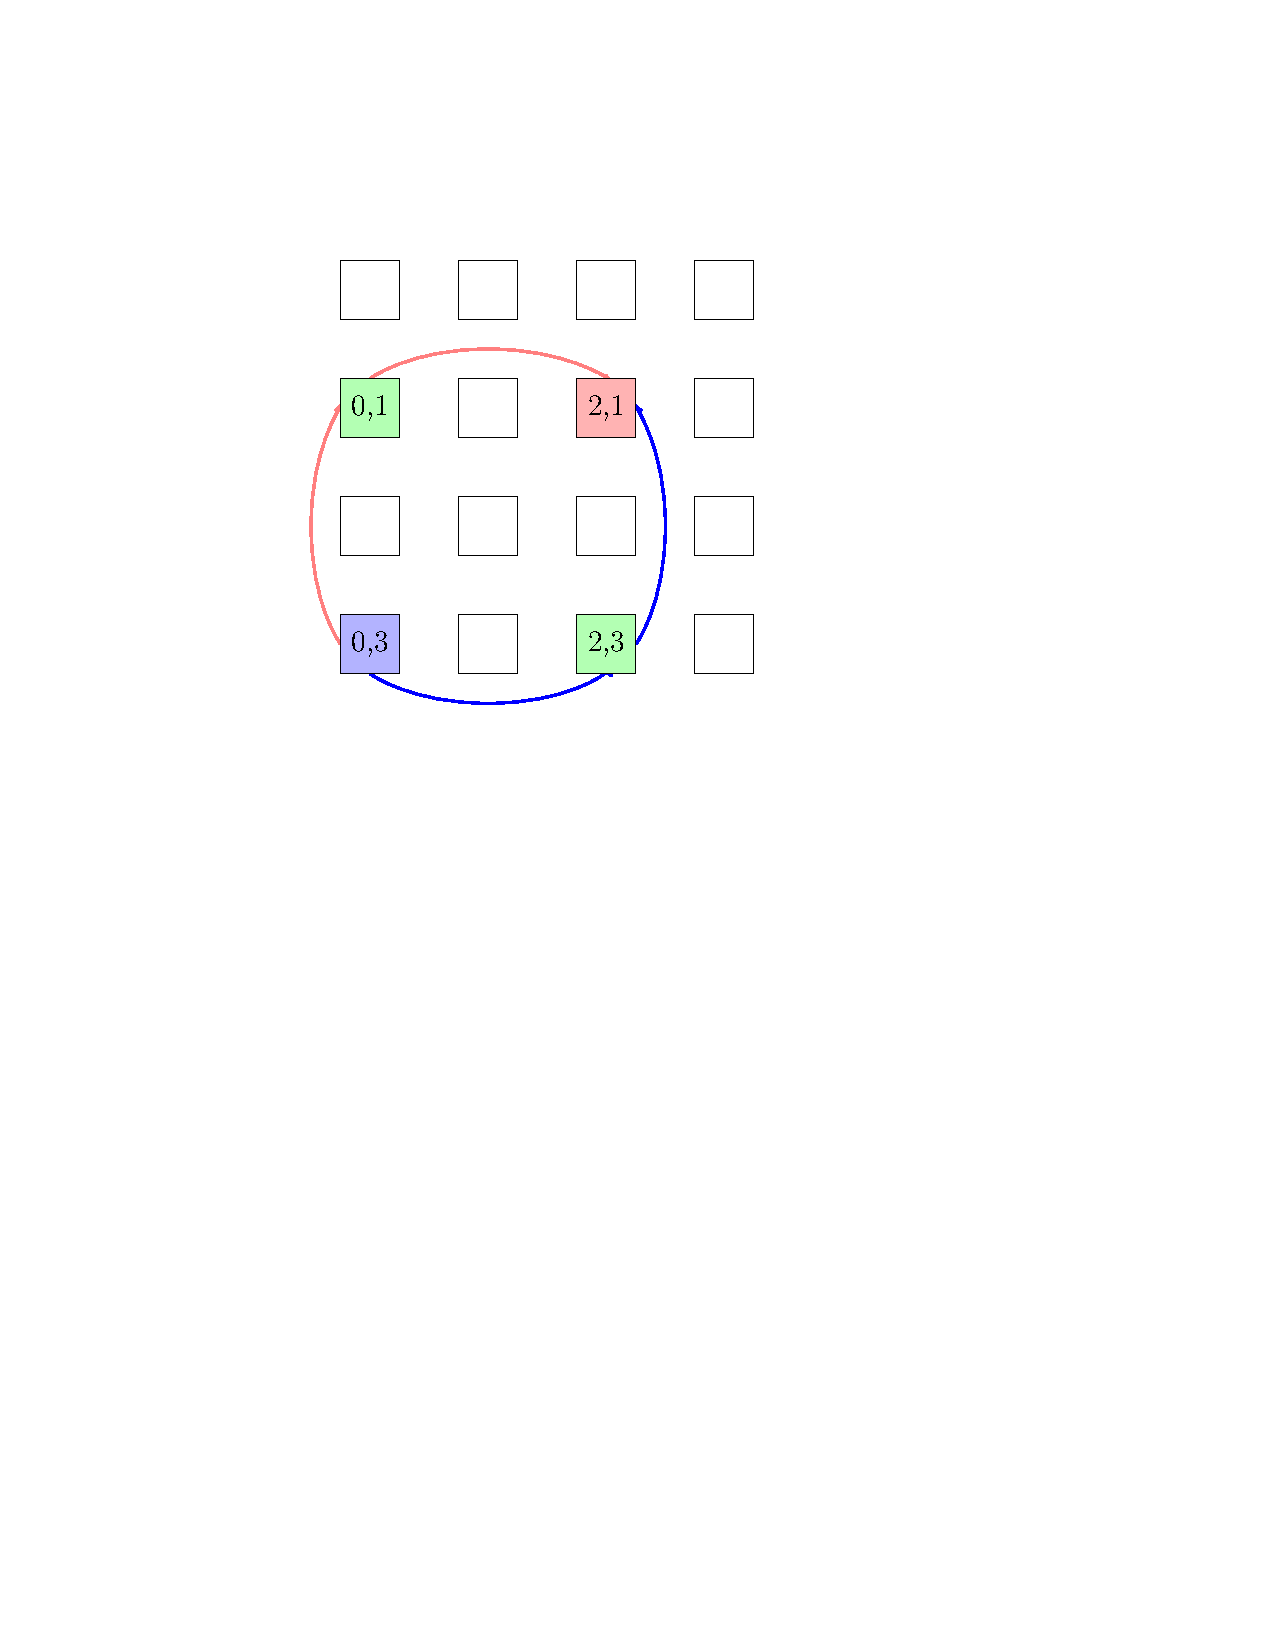
\includegraphics[width=0.5\textwidth]{figures/tikz/hypercube/hypercube_path.pdf}
\caption{Minimal routing within a hypercube showing path diversity. Packet travels from blue to red, passing through green intermediate switches.}
\label{fig:topologies:hypercubePath}
\end{figure}

To fully maximize path diversity on adversarial traffic patterns, though, path-diverse topologies can benefit from Valiant routing.
Here, rather than directly routing to the final destination, packets first route to random intermediate switches on a minimal path.
Then they route again from the intermediate switch to the final destination also on a minimal path (Figure \ref{fig:topologies:hypercubeValiant}).
Although it increases the hop count and therefore the point-to-point latency, it utilizes more paths and therefore increases the effective point-to-point bandwidth.

\begin{figure}[h!]
\centering
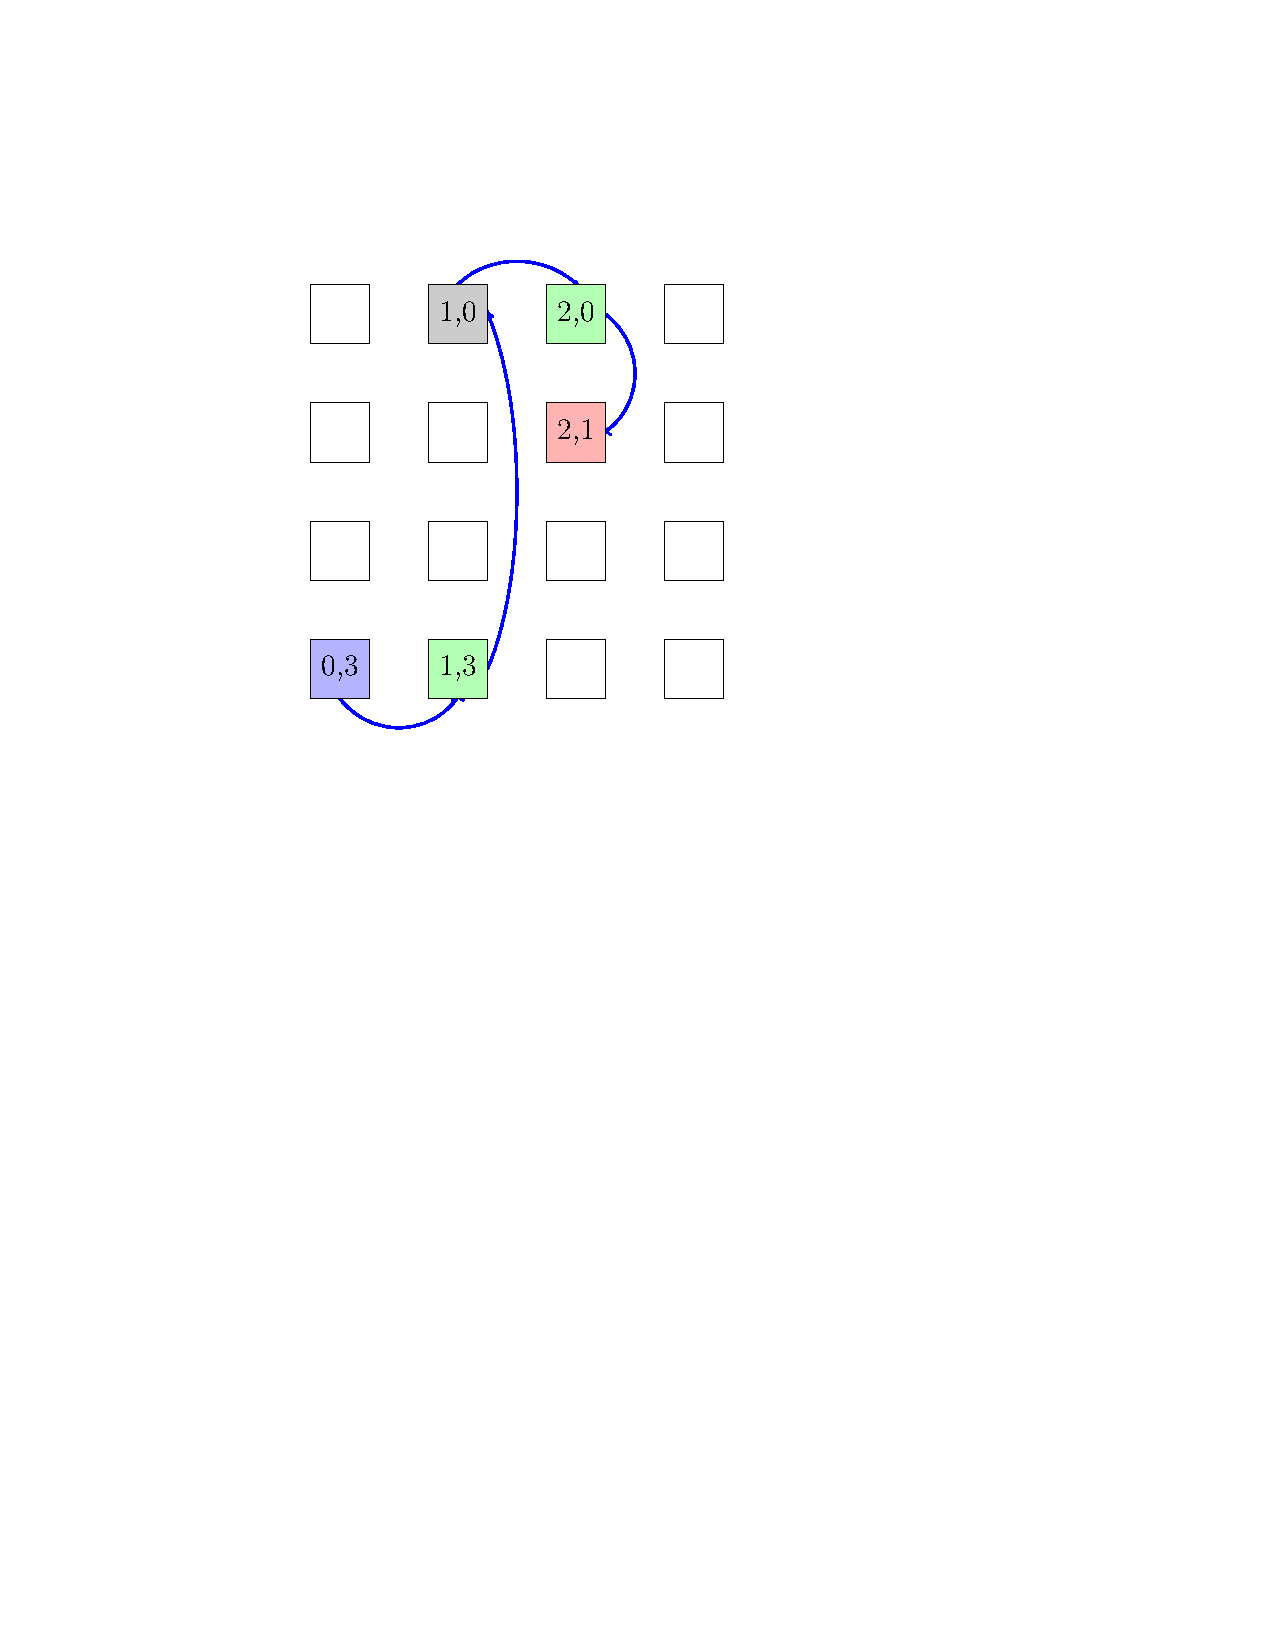
\includegraphics[width=0.5\textwidth]{figures/tikz/hypercube/hypercube_valiant.pdf}
\caption{Valiant routing within a hypercube.  Packet travels from blue to red via a random intermediate destination shown in gray. Additional intermediate switches are shown in green.}
\label{fig:topologies:hypercubeValiant}
\end{figure}

%% !TEX root = manual.tex

\section{Fat Tree}
\label{sec:tutorial:fattree}

SST provides a very flexible fat-tree topology which allows both full bandwidth and tapered bandwidth configurations using either uniform or non-uniform switches.  
This flexibility requires a farily complicated set of input parameters which are best introduced by examining a couple of example configurations.  Consider the full-bandwidth topology in Figure~\ref{fig:topologies:fullfattree} which uses uniform 8-port switches throughout.

\begin{figure}[h!]
\centering
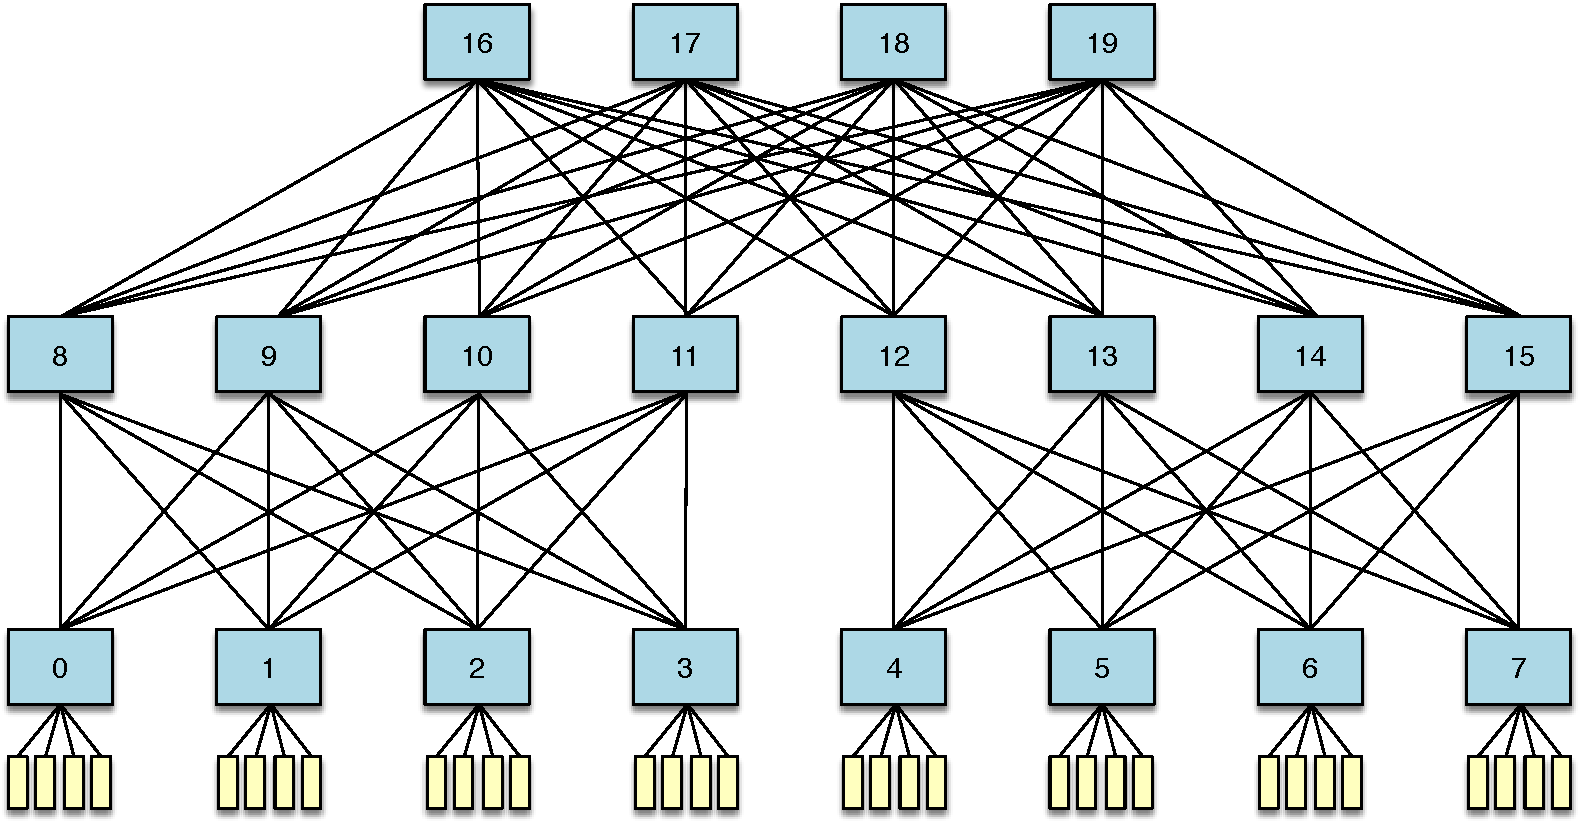
\includegraphics[width=0.7\textwidth]{figures/topologies/fattree4.pdf}
\caption{Full-bandwidth fat-tree topology using uniform 8-port switches.}
\label{fig:topologies:fullfattree}
\end{figure}

The SST fat-tree is strictly a 3-level topology, with the switch levels refered to as leaf (bottom), aggregation (middle), and core (top).
Interconnected leaf and aggregation switches form an aggregation subtree, which forms the basic unit of a fat-tree topology.
The structure of the aggregation subtree is, itself, flexible and places few constraints on the number of subtrees or the way they are connected to the core level.
In Figure~\ref{fig:topologies:fullfattree}, there are 4 leaf switches and 4 aggregation switches per subtree, and each leaf switch has a concentration of four nodes per switch.
Balancing bandwidth, there are 4 ports going up from each leaf switch and 4 ports going down from each aggregation switch.
This subtree can be specified as follows:

\begin{ViFile}
topology.leaf_switches_per_subtree = 4
topology.agg_switches_per_subtree = 4
topology.concentration = 4
topology.up_ports_per_leaf_switch = 4
topology.down_ports_per_agg_switch = 4
\end{ViFile}

In this example we have 2 aggregation subtrees.
There are four ports going up from each aggregation switch.
All of the ports on the core switches go down, so the number of core switches required (4) is only half the number of total aggregation switches (8).
This core configuration can be specified as follows:

\begin{ViFile}
topologies.num_agg_subtrees = 2
topologies.num_core_switches = 4
topologies.up_ports_per_agg_switch = 4
topologies.down_ports_per_core_switch = 8
\end{ViFile}

Putting it all together with the topology name results in:

\begin{ViFile}
topology.name = fat_tree
logy.leaf_switches_per_subtree = 4
topology.agg_switches_per_subtree = 4
topology.concentration = 4
topology.up_ports_per_leaf_switch = 4
topology.down_ports_per_agg_switch = 4
topologies.num_agg_subtrees = 2
topologies.num_core_switches = 4
topologies.up_ports_per_agg_switch = 4
topologies.down_ports_per_core_switch = 8
\end{ViFile}

The next example, though somewhat contrived, better demonstrates the fat-tree input flexibility.
Suppose that one wanted to use the same 8-port switches to construct a 3-level fat-tree that was both cheaper and had more endpoints (nodes), at the cost of interswitch bandwidth.
One possible configuration is shown in Figure~\ref{fig:topologies:taperedfattree}.

\begin{figure}[h!]
\centering
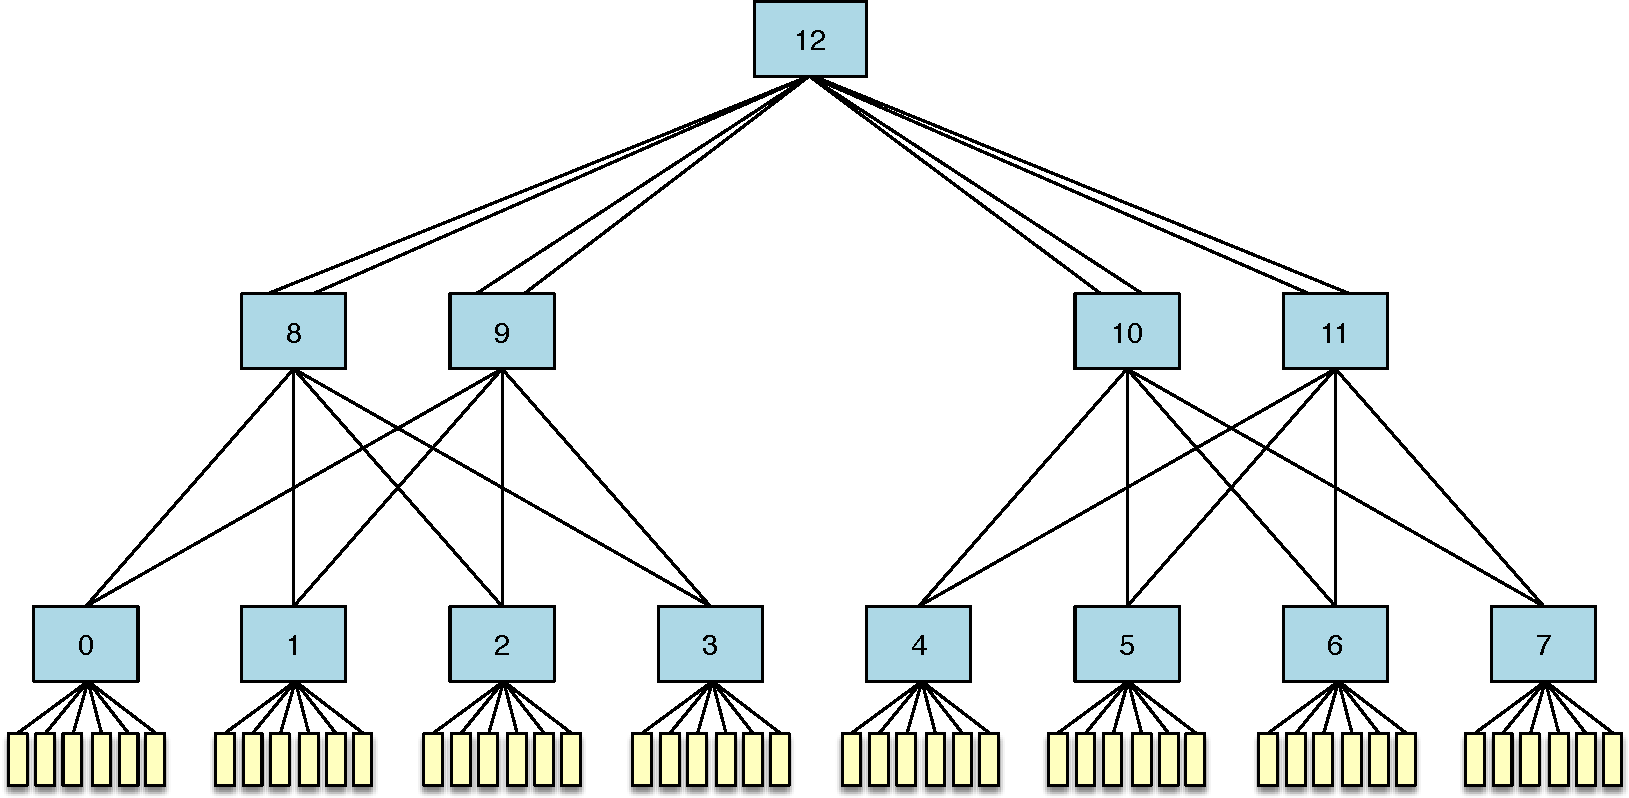
\includegraphics[width=0.7\textwidth]{figures/topologies/fattree4-tapered.pdf}
\caption{A tapered fat-tree topology using uniform 8-port switches.}
\label{fig:topologies:taperedfattree}
\end{figure}

Here the concentration has been increased to 6 nodes per leaf switch, leaving only two up ports per leaf switch.
Thus an aggregation subtree has a total of only 8 leaf up ports, which requires at least two aggregation switches (in order to have any ports left to connect into the core).
Each aggregation switch is then required to have 4 ports heading down.
The subtree can be configured as follows:

\begin{ViFile}
topology.leaf_switches_per_subtree = 4
topology.agg_switches_per_subtree = 2
topology.concentration = 6
topology.up_ports_per_leaf_switch = 2
topology.down_ports_per_agg_switch = 4
\end{ViFile}

There are a total of four aggregation switches.
If the bandwidth is allowed to taper again, a single 8-port core switch can accomodate 2 ports coming up from each aggregation switch.
This core configuration can be specified as follows:

\begin{ViFile}
topologies.num_agg_subtrees = 2
topologies.num_core_switches = 1
topologies.up_ports_per_agg_switch = 2
topologies.down_ports_per_core_switch = 8
\end{ViFile}

This is a heavily tapered tree and also has the downside of using only 6 ports per switch in the aggregation level.
This example was chosen more for its illustrative rather than practical value, though there are certainly applications where it would be perfectly adequate. 
More practical tapering becomes an option when you increase the number of ports per switch, but visualizations become more difficult to grasp.

The following constraints must be met for a valid configuration.
\begin{itemize}
\renewcommand{\labelitemii}{$\circ$}
\item Down ports must equal up ports: leaf up ports (\inlineshell{leaf_switches_per_subtree} $\cdot$ \inlineshell{up_ports_per_leaf_switch}) must equal aggregation down ports (\inlineshell{agg_switches_per_subtree} $\cdot$ \inlineshell{down_ports_per_agg_switch}), and total aggregation up ports (\inlineshell{up_ports_per_agg_switch} $\cdot$ \inlineshell{agg_switches_per_subtree} $\cdot$ \inlineshell{num_agg_subtrees}) must equal total core down ports (\inlineshell{num_core_switches} $\cdot$ \inlineshell{down_ports_per_core_switch}).
\item Need enough down ports -- each switch must have at least one link into each "unit" (subtree or switch, depending on level) below it:  \inlineshell{down_ports_per_core_switch} must be $\geq$ \inlineshell{num_agg_subtrees}, and \inlineshell{down_ports_per_agg_switch} must be $\geq$ \inlineshell{leaf_switches_per_subtree}.
\item Need enough up ports -- each "unit" (subtree or switch) must have at least one link into each switch above it: \inlineshell{up_ports_per_agg_switch} $\cdot$ \inlineshell{agg_switches_per_subtree} must be $\geq$ \inlineshell{num_core_switches}, and \inlineshell{up_ports_per_leaf_switch} must be $\geq$ \inlineshell{agg_switches_per_subtree}.
\item Connections need to be regular:
  \begin{itemize}
  \item \inlineshell{down_ports_per_core_switch} $\bmod$ \inlineshell{num_agg_subtrees} must equal zero
  \item \inlineshell{down_ports_per_agg_switch} $\bmod$ \inlineshell{leaf_switches_per_subtree} must equal zero
  \item \inlineshell{up_ports_per_leaf_switch} $\bmod$ \inlineshell{agg_switches_per_subtree} must equal zero
  \end{itemize}
\end{itemize}

\subsection{Switch Crossbar Bandwidth Scaling}
\label{subsec:fattree:xbarbw}

Allowing non-uniform switches in the topology implies that switch crossbar bandwidth should be non-uniform as well.
By default, SST assumes \inlineshell{switch.xbar.bandwidth} specifies the bandwidth for the switch type with the lowest port count.
The crossbar bandwidth is scaled by the total number of ports for all other switch types. 
Input keywords are provided to override this default behavior.
For the tapered-bandwidth example above, uniform switch bandwidth can be maintained by setting all bandwidth scaling to 1.0:

\begin{ViFile}
topology.leaf_bandwidth_multiplier = 1.0
topology.agg_bandwidth_multiplier = 1.0
topology.core_bandwidth_multiplier = 1.0
\end{ViFile}

\subsection{Routing}
\label{subsec:fattree:routing}

The fat-tree topology should be used in conjunction with \inlineshell{router = fat_tree}, which will maximize the utilization of path diversity.
There is a \inlineshell{fat_tree_minimal} router which will use the lowest numbered valid port for any destination; this will result in poor network performance and is primarily useful for testing and perhaps experiments where network contention is desired.

%% !TEX root = manual.tex

\section{cascade}
\label{sec:tutorial:cascade}

\begin{figure}[h!]
\centering
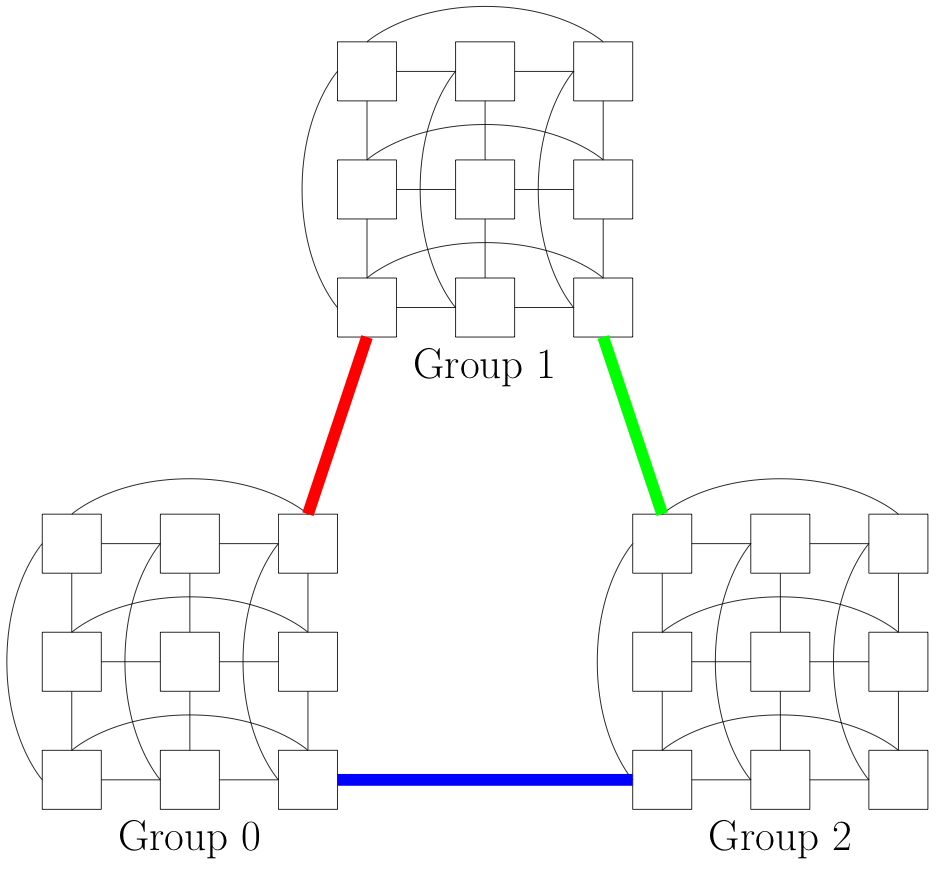
\includegraphics[width=0.7\textwidth]{figures/tikz/cascade/cascade.png}
\caption{Schematic of cascade with three groups showing hypercube intragroup links and high bandwidth intergroup global links}
\label{fig:topologies:cascade}
\end{figure}

As bandwidth per pin increases, arguments can be made that optimal topologies should be higher radix.
A 3D torus is on the low-radix extreme while a hypercube is a high-radix extreme.
A variation on the dragonfly is the cascade topology implemented by Cray on their Aries interconnects.
A cascade is sometimes viewed as a generalization of flattened butterfly and hypercube topologies with ``virtual'' switches of very high radix,
not dissimilar from the fat-tree implementation with many physical commodity switches composing a single virtual switch.
The cascade topology (Figure \ref{fig:topologies:cascade}) is actually quite simple.
Small groups are connected as a generalized hypercube with full connectivity within a row or column.
Intergroup connections (global links) provide pathways for hopping between groups.
A cascade is usually understood through three parameters:
\begin{itemize}
\item $p$: number of nodes connected to each router
\item $a$: number of routers in a group
\item $h$: number of global links that each switch has
\end{itemize}

For simplicity, only three example global links are show for clarity in the picture.
For the Cray X630, $a = 96$, $h=10$, and $p=4$ so that each router is connected to many other ($h=10$) groups.
The caveat is that in many implementations global links are grouped together for $h=2$ or $3$ fat global links.
These demonstrate well-balanced ratios.
In general, scaling out a cascade should not increase the size of a group, only the number of groups.

\subsection{Allocation and indexing}
\label{subsec:cascade:allocatoin}

The cascade coordinate system is essentially the same as a 3D torus.
The group 2D hypercube layout defines $X$ and $Y$ coordinates.
The group number defines a $Z$ or $G$ coordinate.
Thus the topology in Figure \ref{fig:topologies:cascade} would be specified as

\begin{ViFile}
topology.name = cascade
topology.geometry = 3 3 3
\end{ViFile}
for groups of size $3 \times 3$ with a total of 3 groups.
To complete the specification, the number of global links ($h$) for each router must be given

\begin{ViFile}
topology.group_connections = 10
\end{ViFile}

\subsection{Routing}
\label{subsec:cascade:routing}

It is important to understand the distinction between link bandwidth, channel bandwidth, and pin bandwidth.
All topologies have the same pin bandwidth and channel bandwidth (assuming they use the same technology).
Each router in a topology is constrained to have the same number of channels (called radix, usually about $k=64$).
The number of channels per link changes dramatically from topology to topology.
Low radix topologies like 3D torus can allocate more channels per link, 
giving higher bandwidth between adjacent routers.
cascade is higher radix, having many more connections but having lower bandwidth between adjacent routers.
While minimal routing is often sufficient on torus topologies because of the high link bandwidth,
cascade will exhibit very poor performance with minimal routing.
To effectively utilize all the available bandwidth, packets should have a high amount of path diversity.
Packets sent between two routers should take as many different paths as possible to maximize the effective bandwidth point-to-point.

\begin{figure}[h!]
\centering
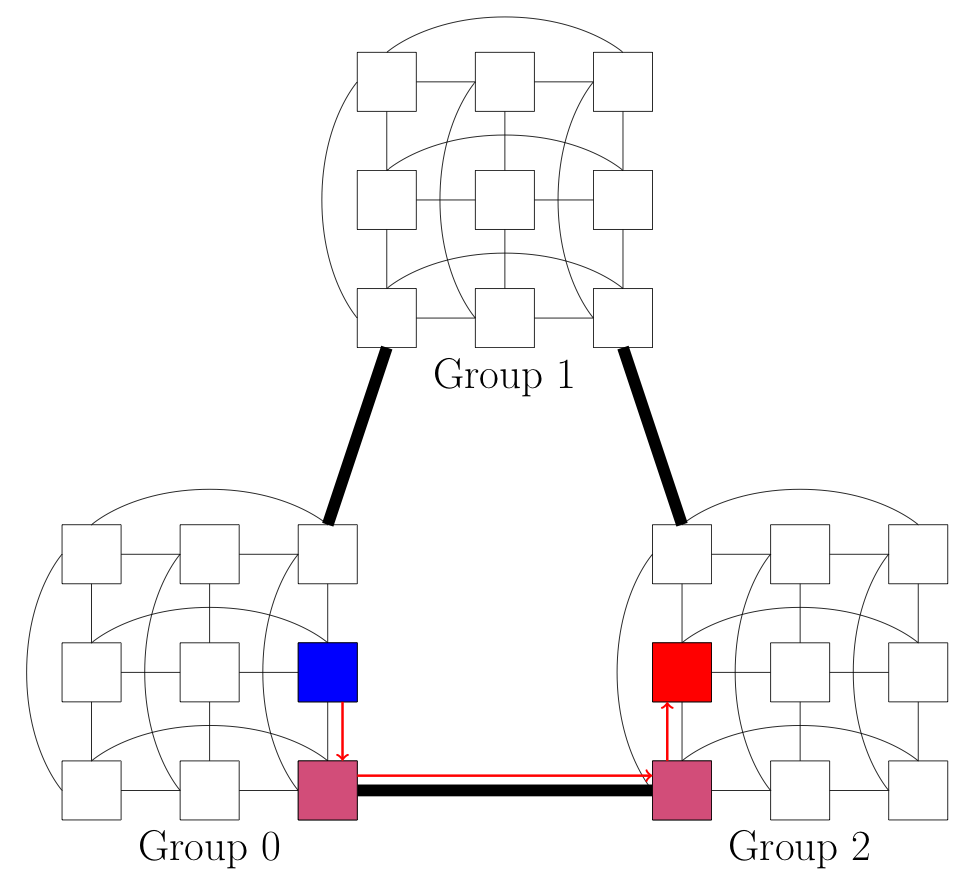
\includegraphics[width=0.7\textwidth]{figures/tikz/cascade/dflyminroute.png}
\caption{Schematic of cascade showing minimal route. Traveling between groups requires routing to the correct global link, hopping the global link, then routing within a group to the correct final node.}
\label{fig:topologies:dflyminroute}
\end{figure}

Minimal routing itself has a few complications (Figure \ref{fig:topologies:dflyminroute}).  
Each router only has a few global links.  
Thus, traveling from e.g. the blue router at X=3,Y=2,G=0 to the red router at X=1,Y=2,G=2, there is no direct link between the routers.
Furthermore, there is no direct link between Groups 0 and 2.
Thus packets must route through the purple intermediate nodes.
First, the packet hops to X=3,Y=3, G=0.  
This router has a global link to Group 2, allowing the packet to hop to the next intermediate router at X=1, Y=3, G=2.
Finally, the minimal route completes by hopping within Group 2 to the final destination.

\begin{figure}[h!]
\centering
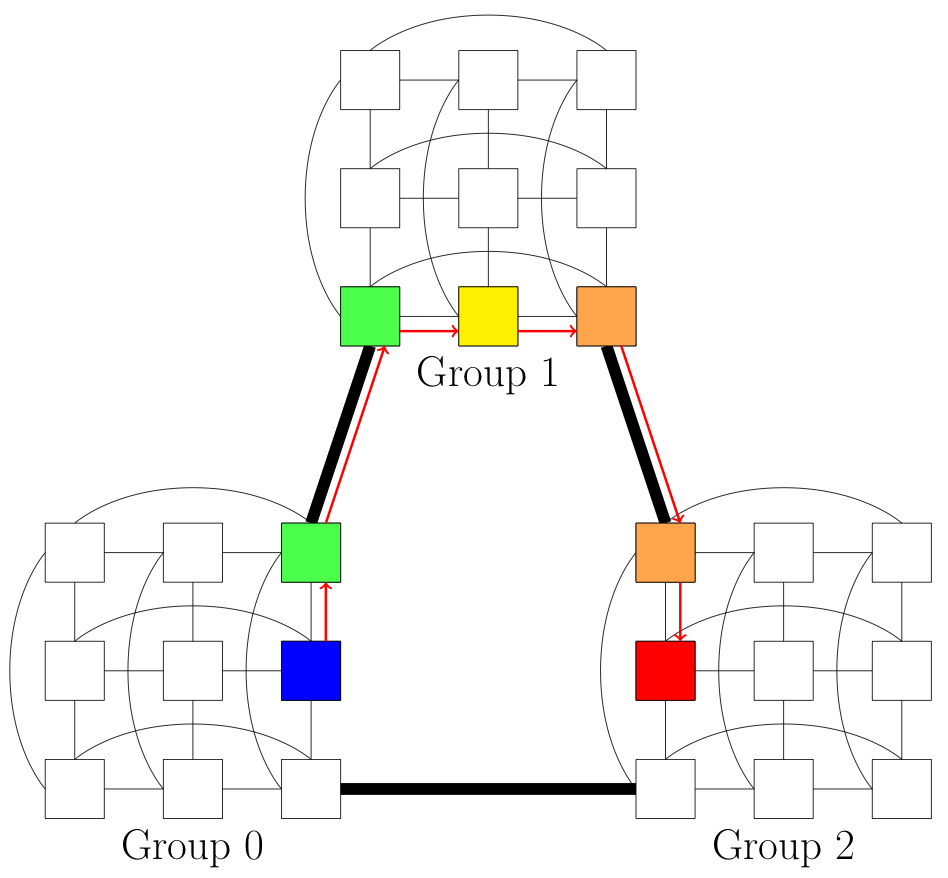
\includegraphics[width=0.7\textwidth]{figures/tikz/cascade/dflyvaliant.png}
\caption{Schematic of cascade showing Valiant route. Traveling between groups requires routing to a random intermediate node, then routing minimally to the final destination.}
\label{fig:topologies:dflyvaliantroute}
\end{figure}

To improve on minimal routing, global routing strategies are required (global routing is distinguished here from adaptive routing).  
Global essentially means ``not minimal'' and spreads packets along many different paths.
The simplest global routing strategy is Valiant routing, which falls in the global, oblivious category (Figure \ref{fig:topologies:dflyvaliantroute}).
Oblivious simply means packets are scattered randomly without measuring congestion.
In Valiant routing, each packet does the following:
\begin{itemize}
\item Pick a random intermediate node 
\item Route minimally to random node
\item Route minimally from random node to destination node
\end{itemize}
This is somewhat counterintuitive at first.
Rather than go directly to the destination node, packets go out of their way to a random node, shown in Figure \ref{fig:topologies:dflyvaliantroute} as the yellow router.
Thus, routing from the blue router in Group 0 to the red router in Group 2 first follows the minimal path (green routers) to the randomly selected yellow router in Group 1. 
From there, a second minimal path is taken through the orange routers to the final destination.
In cases with high congestion or even for large messages on a quiet network, this actually improves performance.
If a point-to-point message is composed of ten packets,
all ten packets will follow different paths to the final destination.
This essentially multiplies the maximum bandwidth by a factor of ten.
Valiant routing can be specified as

\begin{ViFile}
router = valiant
\end{ViFile}

In contrast, UGAL routing is a global, adaptive strategy, making decisions based on congestion.
Because Valiant is oblivious, it often sends too many packets to far away random nodes.
Following a Valiant path is only relevant when enough packets fill up router queues, creating congestion.
UGAL does the following steps:
\begin{itemize}
\item Start routing minimally
\item On each step, check congestion (buffer queue depth)
\item If congestion is too heavy, switch to Valiant and re-route to random intermediate node. Otherwise stay on minimal path.
\end{itemize}
UGAL packets stay on a minimal path until congestion forces them to use a Valiant strategy.
This routing can be specified as:

\begin{ViFile}
router = ugal
\end{ViFile}





% !TEX root = manual.tex

\chapter{Applications and Skeletonization}
\label{sec:skeletonization}

\section{Basic Application porting}
\label{sec:skel:basic}
There are three parts to successfully taking a C++ code and turning it into a running application.
\begin{itemize}
\item Redirected linkage: Rather than linking to MPI, pThreads, or other parallel libraries (or even calling \inlinecode{hostname}), these functions must be redirected to \sstmacro rather than actually executing.
If you compiled with the \inlineshell{--enable-replacement-headers} flag, you get all redirected linkage for free by using
the SST compiler wrappers \inlineshell{sst++} and \inlineshell{sstcc} installed in the \inlineshell{bin} folder.
\item Skeletonization: While \sstmacro can run in emulation mode, executing your entire application exactly, this is not scalable.  To simulate at scale (i.e. 100K or more MPI ranks) you must strip down or ``skeletonize'' the application to the minimal amount of computation.  The energy and time cost of expensive compute kernels are then simulated via models rather than explicitly executed. 

\item Process encapsulation: Each virtual process being simulated is not an actual physical process. It is instead modeled as a lightweight user-space thread.  This means each virtual process has its own stack and register variables, but that is it.
Virtual processes share the same address space and the same global variables.  Some refactoring may be necessary if you have global variables.

\end{itemize}

\section{Redirected linkage}
\label{sec:skel:linkage}
As stated above, in contrast to previous versions, this is essentially automatic now if using the SST compiler wrappers.
The only minor wrinkle is potentially changing the application's entry point, i.e. \inlinecode{main}.
The SST/macro framework has already taken the \texttt{main} function, and consequently the user application becomes a sub-routine within the simulation environment. As introduced in Section~\ref{sec:tutorial:basicmpi}, one needs to change the entry function from \texttt{main} to \texttt{user\_skeleton\_main}, which has the same function signature as the \texttt{main} function.  This refactoring happens automatically in the SST compiler wrappers. 

If you need to use more than one application in the simulator at a time, you need multiple application entry points.
It is no longer possible to do automatic refactoring.  You must explicitly use the macro \inlinecode{sstmac_register_app}
and change the name of your \inlinecode{main}.  Thus, a code might look like

\begin{CppCode}
sstmac_register_app(my_app);

int my_app_main(int argc, char** argv)
{
...
\end{CppCode}
where the refactored \inlinecode{main} function matches the name of the declared application.


\section{Skeletonization}

A program skeleton is a simplified program derived from a parent application. The purpose of a skeleton application is to retain the performance characteristics of interest. At the same time, program logic that is orthogonal to performance properties is removed.  The rest of this chapter will talk about skeletonizing an MPI program, but the concepts mostly apply regardless of what programming/communication model you're using. 

The default method for skeletonizing an application is \textit{manually}. In other words, going through your application and removing all the computation that is not necessary to produce the same communication/parallel characteristics.   Essentially, what you're doing is visually backtracing variables in MPI calls to where they are created, and removing everything else.  

Skeletonization falls into three main categories:

\begin{itemize}
\item \textit{Data structures} - Memory is a precious commodity when running large simulations, so get rid of every memory allocation you can.
\item \textit{Loops} - Usually the main brunt of CPU time, so get rid of any loops that don't contain MPI calls or calculate variables needed in MPI calls.
\item \textit{Communication buffers} - While you can pass in real buffers with data to \sstmacro MPI calls and they will work like normal, it is relatively expensive. If they're not needed, get rid of them.
\end{itemize}

A decent example of skeletonization is HPCCG\_full (the original code) and HPCCG\_skel (the skeleton) in sstmacro/skeletons.  

\subsection{Basic compute modeling}

By default, even if you don't remove any computation, \textit{simulation time doesn't pass between MPI or other calls implemented by \sstmacro} unless you set

\begin{ViFile}
host_compute_modeling = true
\end{ViFile}

in your parameter file.  In this case, \sstmacro will use the wall time that the host takes to run code between MPI calls and use that as simulated time.  This only makes sense, of course, if you didn't do any skeletonization and the original code is all there. 

If you do skeletonize your application and remove computation, you need to replace it with a model of the time or resources necessary to perform that computation so that \sstmacro can advance simulation time properly. 
These functions are all accessible by using the SST compiler wrappers or by adding \inlinefile{#include <sstmac/compute.h>} to your file.

You can describe the time it takes to do computation by inserting calls to 

\begin{ViFile}
void sstmac_compute(double seconds)
\end{ViFile}
Usually, this would be parameterized by some value coming from the application, like loop size.   You can also describe memory movement with 

\begin{ViFile}
void sstmac_memread(long bytes);
void sstmac_memwrite(long bytes);
void sstmac_memcpy(long bytes);
\end{ViFile}
again usually parameterized by something like vector size.  
Using these two functions is the simplest and least flexible way of compute modeling.

\subsection{Detailed compute modeling}
The basic compute modeling is not very flexible.  
In particular, simply computing based on time does not account for congestion delays introduced by things like memory contention.
The highly recommended route is a more detailed compute model (but still very simple) that uses the operational intensity (essentially bytes/flops ratio) for a given compute kernel.
This informs \sstmacro how much stress a given code region puts on either the processor or the memory system.
If a kernel has a very high operational intensity, then the kernel is not memory-bound.
The means multiple threads can be running the kernel with essentially no memory contention.
If a kernel has a very low operational intensity, the kernel is memory bound.
A single thread will have good performance, but multiple threads will compete heavily for memory bandwidth.
If a kernel has a medium operational intensity, a few concurrent threads may be possible without heavy contention, 
but as more threads are added the contention will quickly increase.

The function prototype is

\begin{CppCode}
void
sstmac_compute_detailed(long nflops, long nintops, long bytes);
\end{CppCode}
Here \inlinecode{flops} is the number of floating point operations and \inlinecode{bytes} is the number of bytes that hit the memory controller.
\inlinecode{bytes} is \emph{not} simply the number of writes/reads that a kernel performs.
This is the number of writes/reads that \emph{miss the cache} and hit the memory system.
For now, \sstmacro assumes a single-level cache and does not distinguish between L1, L2, or L3 cache misses.
Future versions may incorporate some estimates of cache hierarchies.
However, given the coarse-grained nature of the simulation, explicit simulation of cache hierarchies is not likely to provide enough improved accuracy or physical insight to justify the increased computational cost. 
Additional improvements are likely to involve adding parameters for pipelining and prefetching.
This is currently the most active area of \sstmacro development.

The characterization of a compute kernel must occur outside \sstmacro using performance analysis tools like Vtune or PAPI.
For the number of flops, it can be quite easy to just count the number of flops by hand.
The number of bytes is much harder.
For simple kernels like a dot product or certain types of stencil computation, 
it may be possible to pen-and-paper derive estimates of the number of bytes read/written from memory since every read is essentially a cache miss.
In the same way, certain kernels that use small blocks (dense linear algebra), it may be possible to reason \textit{a priori} about the cache behavior.
For more complicated kernels, performance metrics might be the only way.
Further discussion and analysis of operational intensity and roofline models can be found in ``Roofline Model Toolkit: A Practical Tool for Architectural and Program Analysis'' by Yung Ju Lo et al.  The PDF is available at \url{http://www.dcs.warwick.ac.uk/~sdh/pmbs14/PMBS14/Workshop_Schedule.html}.

\subsection{Skeletonization Issues}

The main issue that arises during skeletonization is data-dependent communication.  In many cases, it will seem like you can't remove computation or memory allocation because MPI calls depend somehow on that data.  The following are some examples of how we deal with those:

\begin{itemize}
\item \textit{Loop convergence} - In some algorithms, the number of times you iterate through the main loop depends on an error converging to near zero, or some other converging mechanism.  This basically means you can't take out anything at all, because the final result of the computation dictates the number of loops.  In this case, we usually set the number of main loop iterations to a fixed (parameterized) number.  Do we really care exactly how many loops we went through?  Most of the time, no, it's enough just to produce the behavior of the application.  
\item \textit{Particle migration} - Some codes have a particle-in-cell structure, where the spatial domain is decomposed among processes, and particles or elements are distributed among them, and forces between particles are calculated.  When a particle moves to another domain/process (because it's moving through space), this usually requires communication that is different from the force calculation, and thus depends entirely on the data in the application.  We can handle this in two ways:
\begin{enumerate}
\item \textit{Ignore it} - If it doesn't happen that often, maybe it's not significant anyway.  So just remove the communication, recognizing that the behavior of the skeleton will not be fully reproduced.
\item \textit{Approximate it} - If all we need to know is that this migration/communication happens sometimes, then we can just make it happen every so many iterations, or even sample from a probability distribution.  
\end{enumerate}
\item \textit{AMR} - Some applications, like adaptive mesh refinement (AMR), exhibit communication that is entirely dependent on the computation.  In this case, skeletonization is basically impossible, so you're left with the following options:
\begin{itemize}
\item \textit{Traces}  - revert to DUMPI traces, where you will be limited by existing machine size.  Trace extrapolation is also an option here.
\item \textit{Run it} - get yourself a few servers with a lot of memory, and run the whole code in \sstmacro.
\item \textit{Synthetic} - It may be possible to replace communication with randomly-generated data and decisions, which emulate how the original application worked. This hasn't been tried yet.
\item \textit{Hybrid} - It is possible to construct meta-traces that describe the problem from a real run, and read them into \sstmacro to reconstruct the communication that happens.  Future versions of this manual will have more detailed descriptions as we formalize this process.
\end{itemize}
\end{itemize}

\section{Process Encapsulation}

As mentioned above, virtual processes are not real, physical processes inside the OS.
They are explicitly managed user-space threads with a private stack, but without a private set of global variables.
When porting an application to SST/macro, global variables used in C programs will not be mapped to separate memory addresses causing incorrect execution or even segmentation faults.
If you have avoided global variables, there is no major issue.  
If you have read-only global variables with the same value on each machine, there is still no issue.
If you have mutable global variables or read-only variables such as \inlinecode{mpi_rank} that differ across processes,
there is so minor refactoring that needs to be done.

\subsection{Manually refactoring global variables}
\label{sec:skel:globals}
\sstmacro provides a complete set of global variable replacements from 
\inlinecode{\#include <sstmac/sstmac\_global.h>}, which is automatically included the SST compiler wrappers.
Then replace the variable type declaration with the ones that have a \inlinecode{global\_} prefix in the header file.
To use this file, you must compile your application with a C++ compiler as a C++ program.  While most of C++ is backwards-compatible, there are some things that are not, and will require either a compiler flag to relax strictness or quick refactor of some of your syntax.

When printing a global variable with \inlinecode{printf}, the user should explicitly invoke a cast to the primitive type in the function call:

\begin{CppCode}
print("Hello world on rank %d", int(rank));
\end{CppCode}
If not explicitly cast, the \inlinecode{va\_args} function will be misinterpreted and produce an ``Illegal instruction" error.  
This still follows the ``single-source'' principle since whether compiling for \sstmacro or a real machine, the code is still valid.

\subsection{Automatically refactoring global variables}
Tools are currently in use by developers to automatically refactor codes to use no global variables.
This involves running the source code through a compiler tool chain that then creates a \inlinecode{struct}
encapsulating all global variables into thread-specific classes.
This process is only for advanced users and requires developer help.

%\section{Eiger}
%
%The most flexible, but most complex, method for modeling computation is to use the Eiger Statistical Modeling framework to generate performance models that are polled at runtime. These models take as parameters application-level metrics and map them to performance based on statistical models generated from instrumentation data collected off-line from simulation with SST/macro. These models are generated based off empirical data; patterns about the effect variations in the input values have on performance appear as the sample size grows. This means that by collecting instrumentation data for a large range of application problem sizes, the models are capable of extrapolating performance as problem size grows. Typically the input metrics for these models are any values that may have a direct or indirect effect on the performance of the application. For example, it would be safe to assume that the matrix sizes for a matrix multiplication kernel would correlate with execution time, and therefore would be a good candidate for inclusion in instrumentation. The Eiger framework is robust to handling large sets of input metrics, so the rule of thumb is to be liberal when deciding what to include.
%
%The method for polling Eiger models is through
%\begin{ViFile}
%void SSTMAC_compute_eiger(std::map<std::string, double> values, std::string model_name)
%\end{ViFile}
%The \textit{values} parameter maps metric names to their associated values to poll the model \textit{model\_name}. We also provide convenience functions
%\begin{ViFile}
%void SSTMAC_compute_eiger1(std::string model_name, std::string prefix, 
%                           std::string name1, double val1);
%void SSTMAC_compute_eiger2(std::string model_name, std::string prefix, 
%                           std::string name1, double val1, std::string name2, double val2);
%void SSTMAC_compute_eiger3(std::string model_name, std::string prefix, 
%                           std::string name1, double val1, std::string name2, double val2,
%                           std::string name3, double val3);
%\end{ViFile}
%and so on up to 7. For these versions, the \textit{prefix} parameter allows annotating a prefix to the file name containing the model.
%
%Example usage of Eiger in a skeleton is minimd-cpu, found in sstmacro/skeletons.
%
%Please visit \url{https://bitbucket.org/eanger/eiger} for more information on getting, installing, and using Eiger to generate models, as well as methodology for adding instrumentation to your code.
%
%
%
%
%
%\section{Semi-Automatic Skeletonization}
%\label{sec:skel:method}
%
%\noindent The skeletonization process described here is an iterative process to generate a program skeleton from source code. The skeleton extraction process consists of several sub-processes:
%
%\begin{enumerate}
%\item Static code analysis.
%\item User guidance to augment analysis.
%\item API Specification of skeletonization target characteristics.
%\item Code transformation and generation.
%\end{enumerate}
%
%\subsection{Building the Auto-skeletonizer}
%The latest version of the auto-skeletonizer is shipped as part of the ROSE compiler project. It will be build automatically when building the ROSE compiler from source, which can be obtained from GitHub:
%
%\begin{ShellCmd}
%$ git co https://github.com/rose-compiler/edg4x-rose.git
%\end{ShellCmd}
%For detailed instructions on how to build the ROSE compiler, please refer to the ROSE documentation on:\\\url{http://rosecompiler.org/}.
%If an old version of ROSE installation is avaible to your enviroment, the auto-skeletonizer might also be build separeately using the existing ROSE installation.
%First, obtain the source code of the stand alone auto-skeletonizer using git:
%
%\begin{ShellCmd}
%$ git co https://github.com/mjsottile/rose-mpi-skeletons.git rose-mpi-skeletons
%\end{ShellCmd}
%Then modify the makefile inside the \texttt{rose-mpi-skeletons} folder making it pointing to the existing ROSE installation. Edit the first two lines of the makefile as follows:
%
%\begin{ViFile}
%ROSEINSTALL=/path/to/your/rose/installation/dir/
%BOOSTINTALL=/path/to/your/boost/installation/dir/
%\end{ViFile}
%Last, building the executables with the default makefile:
%
%\begin{ShellCmd}
%$ make
%\end{ShellCmd}
%A successful build using either approach should give your three executables: extractMPISkeleton, generateSignatures, and summarizeSignatures. The use of these executables to generate skeleton source code is explained in the following section.
%
%\subsection{Static Analysis}
%
%\noindent In the static analysis phase, the compilation analysis is performed in three parts:
%
%\begin{enumerate}
%
%\item[1.1] Generating summary information for each function in a given compilation unit.
%
%\item[1.2] Combining individual summary files into a larger summary of the program.
%
%\item[1.3] Extraction of the MPI skeleton using the combined summary information.
%
%\end{enumerate}
%
%\noindent In 1.1, in order to generate the summary information of a source program, we can invoke the following tool:
%
%\begin{ShellCmd}
%$  generateSignatures [options] file...
%\end{ShellCmd}
%
%\noindent The command-line options are as follows:
%
%\begin{CppCode}
% -signature:(o|output) filename - Use 'filename' as the output.
% -signature:(d|debug)           - Print debugging messages.
%\end{CppCode}
%
%\noindent In 1.2, we can combine several compilation units from 1.1 to generate a combined signature by invoking the following tool: 
%
%\begin{ShellCmd}
%$  summarizeSignatures [options] <signature files>
%\end{ShellCmd}
%
%\noindent The command-line options are as follows:
%
%\begin{CppCode}
% -summarize:(o|output) filename - Use 'filename' as the output.
% -summarize:(s|spec) filename   - Use 'filename' as API specification.
% -summarize:(d|debug)           - Print debugging messages.
%\end{CppCode}
%
%\noindent The last two options are only needed for debugging.
%
%\noindent The user should specify all the signature files from the previous step of the analysis in a single step. While the generation of the summary is additive, the overall analysis is more efficient if performed in a single step. \\
%
%\noindent In 1.3, the user can extract the program skeleton using the summarized signature file from 1.2 by invoking the following tool: 
%
%\begin{ShellCmd}
%$  extractMPISkeleton [options] file...
%\end{ShellCmd}
%
%\noindent The filenames are skeletonized and the output is written to files with `rose ' prepended to the filenames. \\
%
%\noindent The command line options are these: 
%
%\begin{CppCode}
% -skel:(o|outline)       - Outline everything not in the skeleton.                   
% -skel:(s|spec) filename - Use 'filename' as the specification of the API.
% -skel:(g|sig)  filename - Use 'filename' as the summary information.
% -skel:(d|debug)         - Print debugging messages.
% -skel:(p|pdf)           - Generate PDF of the generated AST.
%\end{CppCode}
%
%\noindent The last two options are only needed for debugging. In order for the analysis to be complete, a signature file generated from the summarizeSignatures tool must be provided.\\
%
%\noindent Current limitations:
%\noindent The skeleton generator supports C and C++ only. Fortran is not supported with this version of the program skeletonization tool.
%
%%%%%%%%%%%%%%%%%%%%%%%%%%%%%%%%%%%%%%%%%%%%%%%%%%%%%%%%%%%%%%%%%%%%%%%%%%%%%
%
%\subsection{User guidance to augment analysis}
%
%In this phase, users can annotate the program skeleton file to augment the code analysis. \\
%
%\noindent Annotations used by this tool are specified in the following format:
%
%\begin{CppCode}
%#pragma skel [specific pragma text here]
%\end{CppCode}
%
%\noindent Currently, three types of data annotation are supported:
%
%\subsubsection{Loop annotations}
%
%It is not uncommon for skeletonized code to no longer have the looping behavior of the parent application. 
%
%To fix any problems stemming from the modified loop behavior, three options for loop annotations are available:
%
%\begin{CppCode}
%#pragma skel loop iterate exactly(n)
%#pragma skel loop iterate atmost(n)
%#pragma skel loop iterate atleast(n)
%\end{CppCode}
%
%These options correspond to forcing an exact, upper, and lower bound on the iteration count. The pragma must be placed immediately preceding the loop of interest. Loops constructed with 'for', 'while', or 'do while' are all supported as well as loops containing break and continue statements.
%
%\subsubsection{Data declaration annotations}
%
%If a program contains an array that should be preserved in the skeleton, it is useful to have control over how it is initialized since often the skeleton will not contain the computation code that populates the array elements.  The initializer pragma allows these element values to be specified.
%
%\begin{CppCode}
%#pragma skel initializer repeat(x)
%int myArray[14];
%\end{CppCode}
%
%(Where 'x' is a C-expression interpreted in the current scope of the program.)
%
%\subsubsection{Conditional statement annotations}
%
%The conditional annotation currently allows programmers to experiment with skeletons that will randomly branch one way or the other with a specified probability.
%
%The general case is:
%
%\begin{CppCode}
%#pragma skel condition prob(p)
%\end{CppCode}
%
%(Where 'p' is a C-expression interpreted in the current scope of the program
%which should be a floating point number between 0 and 1.0.  As noted above,
%floating point constants are not allowed due to current limitations of
%ROSE.)
%
%%%%%%%%%%%%%%%%%%%%%%%%%%%%%%%%%%%%%%%%%%%%%%%%%%%%%%%%%%%%%%%%%%%%%%
%
%\subsection{API Specification of skeletonization points}
%
%The skeleton generator skeletonizes programs relative to one or more API specifications. 
%
%\noindent APIs are specified in a configuration file that uses an s-expression format. Each API call is a sub-expression with the format:
%
%\begin{CppCode}
%(API_FUNCTION_NAME ARGUMENT_COUNT (deptype argA ..) (deptype argB ..) ...)
%\end{CppCode}
%
%The API collection file is specified using the -skel:s
%command line option:
%
%\begin{ShellCmd}
%$ extractMPISkeleton -skel:s /where/is/the/collection/file
%\end{ShellCmd}
%
%\subsection{Outlining}
%
%The skeleton generator can work in an alternate mode, Outlining.  This mode is specified with the following command-line option:
%
%\begin{CppCode}
%  -skel:o
%  -skel:outline
%\end{CppCode}
%
%In this mode, rather than removing the non-skeleton code, the tool will "outline" (move into separate functions, the converse of inlining) all non-skeleton code.
%
%\subsection{Skeleton Behavior Validation}
%\label{sec:skel:validation}
%Skeleton correctness is important in studying the scalability of an application using the skeleton-driven approach. Based on the trace files produced by the DUMPI library in Section~\ref{sec:tutorial:dumpi}, the trace analysis tool creates a statistical report of various metrics and characteristics of the program skeleton.
%
%The trace analysis tool is built as part of the SST/macro package and can be found in the installation directory. The following command will invoke the trace analysis tool on an existing trace file:
%\begin{ShellCmd}
%$ <SSTMAC_INSTALL>/bin/traceanalyzer -v -o report.xml dumpitracer.meta
%\end{ShellCmd}
%A XML report file will be generated after the analyzing process is done. When comparing the report file with one generated from the original applicaiton, the MPI message and traffic count can be used to verify if the desired communication behavior is preserved.

%% !TEX root = manual.tex

\chapter{Detailed Parameter Listings}
\label{chapter:parameters}
The following chapter is organized by parameter namespaces. Tables in each namespace are organized as
\def\arraystretch{1.5}%  1 is the default, change whatever you need

\begin{tabular}{\tableConfig}
\hline
Name (type) & Default if not given & Allowed \newline Values & Description \\
\hline
\end{tabular}

which lists the possible parameter names, allowed values, and brief descriptions.
More detailed descriptions of particular parameter values are found in the documentation in previous chapters.

The allowed parameter types are:

\begin{tabular}{| l | l |}
\hline
int & Any integer \\
\hline
long & Any integer value, but guaranteed not to overflow for long integers \\
\hline
bool & Either ``true'' or ``false'' as lowercase string \\
\hline
time & Any valid float value followed by time units (s,ms,us,ns,ps) \\
\hline
freq & Any valid float value followed by frequency units (Hz, MHz, GHz) \\
\hline
bandwidth & Any valid float value followed by bandwidth units (b/s, B/s, Mb/s, MB/s, etc) \\
\hline
byte length & Any positive integer followed by length units (B, KB, MB, GB,TB) \\
\hline
string & An arbitrary string \\
\hline
vector of X & A vector of type X with entries separated by spaces \\
\hline
filepath & A valid filepath to an \emph{existing} file, either absolute or relative \\
\hline
quantiy & A catch-all for a quantity with units. Any of frequency, bandwidth, byte length, or time can be given \\
\hline
\end{tabular}

\section{Global namespace}
\label{sec:globalParams}

\openTable
\hline
sst\_nthread \paramType{int} & 1 & Positive int & Only relevant for multi-threading. Specifying more threads than cores can lead to deadlock. \\
\hline
timestamp\_resolution \paramType{time} & 1ps & & Specifies the length of time occupied by 1 timestamp tick - the smallest resolvable time difference. Numerical stability depends on this parameter matching the time scales of the simulation. \\
\hline
serialization\_buffer\_size \paramType{byte length} & 16 KB & & Size to allocate for buffering point-to-point sends in parallel. This should set be large enough to handle serialization of all messages in a given time window, but not so large that significant space is wasted. \\
\hline
backup\_buffer\_size \paramType{byte length} & 1 MB & & Size to allocate for special overflow buffers when the standard buffer is overrun. This is the base size and continues to grow if buffers overflow again in a time window. This should be large enough so that buffers do not continuously overflow, but not so large that memory gets filled up. \\
\hline
cpu\_affinity \paramType{vector of int} & No default & Invalid cpu IDs give undefined behavior & When in multi-threading, specifies the list of core IDs that threads will be pinned to. \\
\hline
\end{tabular}

\section{Namespace ``topology''}
\label{sec:topologyParams}

\openTable
\hline
geometry \paramType{vector of int} & No default & See Topology section & Geometry configuration of the topology. For details of the keyword, users should refer to Section \ref{chapter:topologies} \\
\hline 
auto \paramType{bool} & false & Whether to auto-generate the topology based on the application size. \\
\hline
name \paramType{string} & No default & torus, cascade, dragonfly, fat\_tree, crossbar, tapered\_fat\_tree & The name of the topology to build. For details, see Section \ref{chapter:topologies} \\
\hline 
seed \paramType{long} & System time & & If no value given, random numbers for topology will be generated from system time \\
\hline
concentration \paramType{int} & 1 & Positive int & The number of nodes per network switch. For indirect networks, this is the number of nodes per leaf switch. \\
\hline
num\_leaf\_switches \paramType{int} & No default & Positive int & Only relevant for fat trees. This is the number of switches at the lowest level of the tree that are connected to compute nodes. Depending on how the fat tree is specified, this number may not be required. \\
\hline
k \paramType{int} & No default & int >= 2 & The branching fraction of a fat tree. k=2 is a binary tree. k=4 is a quad-tree. \\
\hline
l \paramType{int} & No default & Positive int & The number of levels in a fat tree. \\
\hline
num\_inj\_switches\_per\_subtree & No default & Positive int & For a tapered tree, the number of injection switches, $N_{inj}$, within an aggregation tree that connect directly toc ompute nodes. \\
\hline
num\_agg\_switches\_per\_subtree & No default & Positive int & For a tapered tree, the number of aggregations witches per aggregation tree linking injection switches to the core. \\
\hline
num\_agg\_subtrees & No default & Positive int & For a tapered fat tree with 3 levels (injection, aggregation, core), this gives the number, $N_{agg}$, of aggregation subtrees. To find the total number, $N_{tot}$ of injection (leaf) switches, we have $N_{tot} = N_{agg} \times N_{inj}$. \\
\hline
num\_core\_switches & No default & Positive int & The total number of core switches in a tapered tree linking the individual aggregation trees. \\
\hline
group\_connections \paramType{int} & No default & Positive int & For cascase ir dragonfly, the number of intergroup connections on each switch in a Dragonfly group \\
\hline
redundant \paramType{vector of int} & vector of 1's & Positive ints & For Cartesian topologies (hypercube, cascadem, dragonfly, torus) this specifies a bandwidth (redundancy) multiplier for network links in each dimension. \\
\hline
\end{tabular}

\section{Namespace ``node''}
\label{sec:nodeParams}

\openTable
\hline
name \paramType{string} & simple & simple & The type of node model (level of detail) for node-level operations \\
\hline
services \paramType{vector of strings} & Empty & Valid service names & For  details, see section on distributed services in developer's manual. Advanced feature. \\
\hline
\end{tabular}

\subsection{Namespace ``node.nic''}
\label{subsec:node:nic:Params}

\openTable
\hline
name \paramType{string} & No default & pisces, logP & The type of NIC model (level of detail) for modeling injection of messages (flows) to/from the network. \\
\hline
packetizer \paramType{string} & cut\_through & merlin, simple, cut\_through & The type of packetizer for injecting flows into the network. Merlin is part of sst-elements. Simple and cut-through use PISCES \\
\hline
negligible\_size \paramType{byte length} & 256B & & Messages (flows) smaller than size will not go through detailed congestion modeling. They will go through a simple analytic model to compute the delay. \\
\hline
\end{tabular}

\subsubsection{Namespace ``node.nic.delay\_histogram''}
\label{subsubsec:node:nic:delayHistogram:Params}
\openTable{8cm}
\hline
fileroot & string & No default & & 
  The path of a file to be created (or overwritten) where results from the statistics will be placed.  \\
\hline
bin\_size & quantiy & No default & Positive value & For the quantity being collected (bytes,time,etc), this determines how large a value range should be binned together. \\
\hline
num\_bins & int & 20 & Positive int & Determines the number of initial bins to allocate. If number is too small, simulation will allocate more. This is just a guess for optimization. \\
\hline
logarithmic & bool & false & & Whether to use a logarithmic axis for binning. \\
\hline
\end{tabular}


\subsubsection{Namespace ``node.nic.congestion\_spyplot''}
\label{subsubsec:node:nic:congestionSpyplot:Params}
\openTable{8cm}
\hline
fileroot & string & No default & & 
  The path of a file to be created (or overwritten) where results from the statistics will be placed.  \\
\hline
normalization & long & Ignored & Positive int & Determines a normalization value that will effect the color scales of an output PNG file. By default, if not specified, the spyplot will determine the largest value and normalize all values for the output PNG to be 0.0-1.0. Values larger than 1.0 will have the same color as 1.0. Useful for having two PNG files with different values have the same color scales. \\
\hline
\end{tabular}


\subsubsection{Namespace ``node.nic.traffic\_matrix''}
\label{subsubsec:node:nic:trafficMatrix:Params}
\openTable{8cm}
\hline
fileroot & string & No default & & 
  The path of a file to be created (or overwritten) where results from the statistics will be placed.  \\
\hline
normalization & long & Ignored & Positive int & Determines a normalization value that will effect the color scales of an output PNG file. By default, if not specified, the spyplot will determine the largest value and normalize all values for the output PNG to be 0.0-1.0. Values larger than 1.0 will have the same color as 1.0. Useful for having two PNG files with different values have the same color scales. \\
\hline
\end{tabular}


\subsubsection{Namespace ``node.nic.local\_bytes\_sent''}
\label{subsubsec:node:nic:localSent:Params}
\openTable
\hline
fileroot & string & No default & & 
  The path of a file to be created (or overwritten) where results from the statistics will be placed.  \\
\hline
\end{tabular}


\subsubsection{Namespace ``node.nic.global\_bytes\_sent''}
\label{subsubsec:node:nic:globalSent:Params}
\openTable
\hline
fileroot & string & No default & & 
  The path of a file to be created (or overwritten) where results from the statistics will be placed.  \\
\hline
\end{tabular}


\subsubsection{Namespace ``node.nic.message\_size\_histogram''}
\label{subsubsec:node:nic:sizeHistogram:Params}
\openTable{8cm}
\hline
fileroot & string & No default & & 
  The path of a file to be created (or overwritten) where results from the statistics will be placed.  \\
\hline
bin\_size & quantiy & No default & Positive value & For the quantity being collected (bytes,time,etc), this determines how large a value range should be binned together. \\
\hline
num\_bins & int & 20 & Positive int & Determines the number of initial bins to allocate. If number is too small, simulation will allocate more. This is just a guess for optimization. \\
\hline
logarithmic & bool & false & & Whether to use a logarithmic axis for binning. \\
\hline
\end{tabular}


\subsubsection{Namespace ``node.nic.ejection"}
\label{subsubsec:node:nic:ejection:Params}
These parameters do not need to be specified, but can be given.
Generally, the simulation assumes an infinite buffer size (unlimited memory) and no latency.
All other parameters can be filled in from \inlinefile{node.nic.injection}.

\openTable
\hline
stats \paramType{string} & null & 
	delay\_histogram,
  congestion\_spyplot,
  multi,
	null 
 & The type of statistics to collect from packets leaving or arriving at the NIC.
   Null indicates no statistics collected. For details on the other types of statistics, see Section \ref{sec:tutorials:packetStats} \\
\hline
callbacks \paramType{vector of string} & No default & Any valid stats name & If \inlinefile{stats} is set to \inlinefile{multi},then multiple different stats can be given here \\
\hline
arbitrator \paramType{string} & cut\_through & null, simple, cut\_through & Bandwidth arbitrator for PISCES congestion modeling. Null uses simple delays with no congestion. Simple uses store-and-forward that is cheap to compute, but can have severe latency errors for large packets. Cut-through approximates pipelining of flits across stages.  \\
\hline
latency \paramType{time} & No default & & If given, overwrites the send and credit latency parameters. Depending on component, the entire latency may be put on either the credits or the send. \\
\hline
bandwidth & No default & & The bandwidth of the arbitrator \\
\hline
send\_latency \paramType{time} & No default & & The latency to send a packet to the next stage in the network. This can be omitted if the generic latency parameter is given (see above). \\
\hline
credit\_latency \paramType{time} & No default & & The latency to send a credit to the previous network stage. This can be omitted if the generic latency parameter is given (see above). \\
\hline
credits \paramType{byte length} & No default & & The number of initial credits for the component. Corresponds to an input buffer on another component. In many cases, SST/macro can compute this from other parameters and fill in the value. In some cases, it will be required. \\
\hline
mtu \paramType{byte length} & 1024B & & The packet size. All messages (flows) will be broken into units of this size. \\

 
\hline
\end{tabular}

\subsubsection{Namespace ``node.nic.injection"}
\label{subsubsec:node:nic:injection:Params}

\openTable
\hline
stats \paramType{string} & null & 
	delay\_histogram,
	null 
 & The type of statistics to collect from packets leaving or arriving at the NIC.
   Null indicates no statistics collected. For details on the other types of statistics, see Section \ref{sec:tutorials:packetStats} \\
arbitrator \paramType{string} & cut\_through & null, simple, cut\_through & Bandwidth arbitrator for PISCES congestion modeling. Null uses simple delays with no congestion. Simple uses store-and-forward that is cheap to compute, but can have severe latency errors for large packets. Cut-through approximates pipelining of flits across stages.  \\
\hline
latency \paramType{time} & No default & & If given, overwrites the send and credit latency parameters. Depending on component, the entire latency may be put on either the credits or the send. \\
\hline
bandwidth & No default & & The bandwidth of the arbitrator \\
\hline
send\_latency \paramType{time} & No default & & The latency to send a packet to the next stage in the network. This can be omitted if the generic latency parameter is given (see above). \\
\hline
credit\_latency \paramType{time} & No default & & The latency to send a credit to the previous network stage. This can be omitted if the generic latency parameter is given (see above). \\
\hline
credits \paramType{byte length} & No default & & The number of initial credits for the component. Corresponds to an input buffer on another component. In many cases, SST/macro can compute this from other parameters and fill in the value. In some cases, it will be required. \\
\hline
mtu \paramType{byte length} & 1024B & & The packet size. All messages (flows) will be broken into units of this size. \\

 
\hline
\end{tabular}


\subsection{Namespace ``node.memory''}
\label{subsec:node:memory:Params}

\openTable
\hline
model \paramType{string} & No default & logP, pisces & The type of memory model (level of detail) for modeling memory transactions. \\
\hline
arbitrator \paramType{string} & cut\_through & null, simple, cut\_through & The type of arbitrator. See arbitrator descriptions above. \\
\hline
latency \paramType{time} & No default & & The latency of single memory operation \\
\hline
total\_bandwidth & No default &  & The total memory bandwidth possible across all memory controllers. \\
\hline
max\_single\_bandwidth & Computed & & The maximum memory bandwidth of a single stream of requests. Essentially the bandwidth of a single memory controller. If not given, this defaults the value of total\_bandwidth. \\
\hline
\end{tabular}

\subsection{Namespace ``node.os"}
\label{subsec:node:os:Params}

\openTable
\hline
compute\_scheduler \paramType{string} & simple & simple, cpuset & The level of detail for scheduling compute tasks to cores. Simple looks for any empty core. cpuset allows bitmasks to be set for defining core affinities. \\
\hline
stack\_size \paramType{byte length} & 64 KB & & The size of user-space thread stack to allocate for each virtual application \\
\hline
stack\_chunk\_size \paramType{byte length} & 1 MB & & The size of memory to allocate at a time when allocating new thread stacks. Rather than allocating one thread stack at a time, multiple stacks are allocated and added to a pool as needed.  \\
\hline
\end{tabular}

\subsubsection{Namespace ``node.os.call\_graph"}
\label{subsubsec:node:os:callGraph:Params}
\openTable
\hline
fileroot & string & No default & & 
  The path of a file to be created (or overwritten) where results from the statistics will be placed.  \\
\hline
\end{tabular}

\subsubsection{Namespace ``node.os.ftq"}
\label{subsubsec:node:os:ftq:Params}
\openTable
\hline
fileroot & string & No default & & 
  The path of a file to be created (or overwritten) where results from the statistics will be placed.  \\
\hline 
epoch \paramType{time} & No default & & The length of simulation time to treat as a single interval. This is much like a histogram bin, except the bin is partitioned into multiple categories. If too small, not enough data will be collected per interval to give reasonable looking results. If too large, significant changes in system activity over time will not be resolved. \\
\hline
\end{tabular}

\subsection{Namespace ``node.proc''}
\label{subsec:node:proc:Params}
\openTable
\hline
ncores \paramType{int} & No default & Positive int & The number of cores contained in a processor (socket). Total number of cores for a node is $ncores \times nsockets$. \\
\hline
frequency & No default & & The baseline frequency of the node \\
\hline
parallelism \paramType{double} & 1.0 & Positive number & Fudge factor to account for superscalar processor. Number of flops per cycle performed by processor. \\
\hline
\end{tabular}

\section{Namespace ``mpi"}
\label{sec:mpi:Params}

\openTable
\hline
test\_delay \paramType{time} & 0 & & The minimum time spent by MPI on each MPI\_Test call \\
\hline
iprobe\_delay \paramType{time} & 0 & & The minimum time spent by MPI on each MPI\_Iprobe call \\
\hline
otf2\_dir\_basename \paramType{time} & empty string & & Enables OTF2 and combines this parameter with a timestamp to name the archive \\
\hline
\end{tabular}

\subsection{Namespace ``mpi.queue''}
\label{subsec:mpi:queue:Params}

\openTable
\hline
max\_vshort\_msg\_size \paramType{byte length} & 512B & & The maximum size to use the very short message protocol. Small messages are sent eagerly using special pre-allocated mailbox buffers. Sends complete immediately. \\
\hline
max\_eager\_msg\_size \paramType{byte length} & 8KB & & The maximum size to use the RDMA eager protocol. This also uses buffers to send message, but instead of using pre-allocated mailboxes, it coordinates an RDMA get. Sends complete immediately. \\
\hline
post\_rdma\_delay \paramType{time} & 0 & & The minimum time spent by MPI posting each RDMA operation \\
\hline
post\_header\_delay \paramType{time} & 0 & & The mimimum time spent by MPI sending headers into pre-allocated mailboxes \\
\hline
poll\_delay (time) & 0 & & The minimum time spent by MPI each time it polls for incoming messages \\
\hline
\end{tabular}

\section{Namespace ``switch''}
\label{subsec:switch:Params}

\openTable
\hline
model \paramType{string} & No default & logP, pisces & The type of switch model (level of detail) for modeling network traffic. \\
\hline
buffer\_size \paramType{byte length} & No default & & The size of input and output buffers on each switch. This determines the number of credits available to other components \\
\hline
\end{tabular}

\subsection{Namespace ``switch.router''}
\label{subsec:switch:router:Params}

\openTable
\hline
name \paramType{string} & No default & minimal, valiant, ugal, dragonfly\_minimal, fat\_tree & The name of the routing algorithm to use for routing packets. \\
\hline
ugal\_threshold \paramType{int} & 0 & & The minimum number of network hops required before UGAL is considered. All path lengths less than value automatically use minimal. \\
\hline
\end{tabular}

\subsection{Namespace ``switch.output\_buffer"}
\label{subsec:switch:outputBuffer:Params}

\openTable
\hline
stats \paramType{string} & null & 
	delay\_histogram,
  byte\_hops,
	null 
 & The type of statistics to collect from packets leaving or arriving at the switch output buffers.
   Null indicates no statistics collected. For details on the other types of statistics, see Section \ref{sec:tutorials:packetStats} \\
\hline
\end{tabular}

\subsubsection{Namespace ``switch.output\_buffer.delay\_histogram''}
\label{subsubsec:switch:outputBuffer:delayHistogram:Params}
\openTable{8cm}
\hline
fileroot & string & No default & & 
  The path of a file to be created (or overwritten) where results from the statistics will be placed.  \\
\hline
bin\_size & quantiy & No default & Positive value & For the quantity being collected (bytes,time,etc), this determines how large a value range should be binned together. \\
\hline
num\_bins & int & 20 & Positive int & Determines the number of initial bins to allocate. If number is too small, simulation will allocate more. This is just a guess for optimization. \\
\hline
logarithmic & bool & false & & Whether to use a logarithmic axis for binning. \\
\hline
\end{tabular}


\subsubsection{Namespace ``switch.output\_buffer.byte\_hops''}
\label{subsubsec:switch:outputBuffer:delayHistogram:Params}
\openTable
\hline
fileroot & string & No default & & 
  The path of a file to be created (or overwritten) where results from the statistics will be placed.  \\
\hline
\end{tabular}


\subsection{Namespace ``switch.xbar"}
\label{sec:switch:outputBuffer:delayHistogram:Params}

\openTable
\hline
stats \paramType{string} & null & 
	bytes\_sent,
	null 
 & The type of statistics to collect from packets leaving or arriving at the switch crossbar.
   Null indicates no statistics collected. For details on the other types of statistics, see Section \ref{sec:tutorials:packetStats} \\
\hline
arbitrator \paramType{string} & cut\_through & null, simple, cut\_through & Bandwidth arbitrator for PISCES congestion modeling. Null uses simple delays with no congestion. Simple uses store-and-forward that is cheap to compute, but can have severe latency errors for large packets. Cut-through approximates pipelining of flits across stages.  \\
\hline
latency \paramType{time} & No default & & If given, overwrites the send and credit latency parameters. Depending on component, the entire latency may be put on either the credits or the send. \\
\hline
bandwidth & No default & & The bandwidth of the arbitrator \\
\hline
send\_latency \paramType{time} & No default & & The latency to send a packet to the next stage in the network. This can be omitted if the generic latency parameter is given (see above). \\
\hline
credit\_latency \paramType{time} & No default & & The latency to send a credit to the previous network stage. This can be omitted if the generic latency parameter is given (see above). \\
\hline
credits \paramType{byte length} & No default & & The number of initial credits for the component. Corresponds to an input buffer on another component. In many cases, SST/macro can compute this from other parameters and fill in the value. In some cases, it will be required. \\
\hline
mtu \paramType{byte length} & 1024B & & The packet size. All messages (flows) will be broken into units of this size. \\


\hline
\end{tabular}

\subsubsection{Namespace ``switch.xbar.bytes\_sent''}
\label{subsubsec:switch:xbar:bytesSent:Params}
\openTable
\hline
fileroot & string & No default & & 
  The path of a file to be created (or overwritten) where results from the statistics will be placed.  \\
\hline
\end{tabular}


\subsection{Namespace ``switch.link''}
\label{subsec:switch:link:Params}
\openTable{8cm}
\hline
arbitrator \paramType{string} & cut\_through & null, simple, cut\_through & Bandwidth arbitrator for PISCES congestion modeling. Null uses simple delays with no congestion. Simple uses store-and-forward that is cheap to compute, but can have severe latency errors for large packets. Cut-through approximates pipelining of flits across stages.  \\
\hline
latency \paramType{time} & No default & & If given, overwrites the send and credit latency parameters. Depending on component, the entire latency may be put on either the credits or the send. \\
\hline
bandwidth & No default & & The bandwidth of the arbitrator \\
\hline
send\_latency \paramType{time} & No default & & The latency to send a packet to the next stage in the network. This can be omitted if the generic latency parameter is given (see above). \\
\hline
credit\_latency \paramType{time} & No default & & The latency to send a credit to the previous network stage. This can be omitted if the generic latency parameter is given (see above). \\
\hline
credits \paramType{byte length} & No default & & The number of initial credits for the component. Corresponds to an input buffer on another component. In many cases, SST/macro can compute this from other parameters and fill in the value. In some cases, it will be required. \\
\hline
mtu \paramType{byte length} & 1024B & & The packet size. All messages (flows) will be broken into units of this size. \\


\hline
\end{tabular}


\subsection{Namespace ``switch.ejection''}
\label{subsec:switch:ejection:Params}
This namespace is not actually required. 
If unspecified, all of the values here will be filled in from \inlinefile{nic.injection}.

\openTable{8cm}
\hline
arbitrator \paramType{string} & cut\_through & null, simple, cut\_through & Bandwidth arbitrator for PISCES congestion modeling. Null uses simple delays with no congestion. Simple uses store-and-forward that is cheap to compute, but can have severe latency errors for large packets. Cut-through approximates pipelining of flits across stages.  \\
\hline
latency \paramType{time} & No default & & If given, overwrites the send and credit latency parameters. Depending on component, the entire latency may be put on either the credits or the send. \\
\hline
bandwidth & No default & & The bandwidth of the arbitrator \\
\hline
send\_latency \paramType{time} & No default & & The latency to send a packet to the next stage in the network. This can be omitted if the generic latency parameter is given (see above). \\
\hline
credit\_latency \paramType{time} & No default & & The latency to send a credit to the previous network stage. This can be omitted if the generic latency parameter is given (see above). \\
\hline
credits \paramType{byte length} & No default & & The number of initial credits for the component. Corresponds to an input buffer on another component. In many cases, SST/macro can compute this from other parameters and fill in the value. In some cases, it will be required. \\
\hline
mtu \paramType{byte length} & 1024B & & The packet size. All messages (flows) will be broken into units of this size. \\


\hline
\end{tabular}


\section{Namespace ``appN''}
\label{sec:appN:Params}
This is a series of namespaces \inlineshell{app1}, \inlineshell{app2}, and so on for each of the launched applications. These should be contained within the \inlineshell{node} namespace.

\openTable
\hline
name \paramType{string} & No default & parsedumpi, cxx\_full\_main, cxx\_empty\_main & The name of the application to launch. Very few applications are built-in. Registration of external apps is shown starting in Section \ref{sec:tutorial:basicmpi}. \\
\hline
size \paramType{int} & No default & Positive int & The number of procs (MPI ranks) to launch. If launch\_cmd given, this parameter is not required. \\
\hline
start \paramType{int} & 0 & & The time at which a launch request for the application will be made \\
\hline
concentration \paramType{int} & 1 & Positive int & The number of procs (MPI ranks) per compute node \\
\hline
core\_affinities \paramType{vector of int} & Empty & & \\
\hline
launch\_cmd \paramType{string} & No default & Valid aprun or srun & This uses a launch command as would be found with ALPS or SLURM launchers on real systems, e.g. aprun -n 4 -N 1 \\
\hline
indexing \paramType{string} & block & block, random, cart, node\_id, coordinate & The indexing scheme for assign proc ID (MPI rank number) to compute nodes \\
\hline
node\_id\_mapper\_file \paramType{filepath} & No default & & If using Node ID indexing, the file containing the node ID index list \\
\hline 
random\_indexer\_seed \paramType{long} & System time & & The seed to use for a random allocation. If not specified, system time is used. \\
\hline
allocation \paramType{string} & first\_available & first\_available, random, cart, node\_id, coordinate & The scheme to use for allocating compute nodes to a given job. \\
\hline
random\_allocation\_seed \paramType{long} & System time & & For random allocation policy. If unspecified, system time is used as the seed.  \\
\hline
node\_id\_allocation\_file \paramType{filepath} & No default & & If using Node ID allocation, the file containing the list of node IDs to allocate for the job \\
\hline
dumpi\_metaname \paramType{filepath} & No default & & If running DUMPI trace, the location of the metafile for configuring trace replay \\ 
\hline
coordinate\_file \paramType{filepath} & No default & & If running using coordinate allocation or indexing, the path to the file containing the node coordinates of each proc (MPI rank) \\ 
\hline
cart\_sizes \paramType{vector of int} & No default & & Launch a contiguous block of nodes in a Cartesian topology. This gives the size of each dimension in the block. \\
\hline 
cart\_offsets \paramType{vector of int} & No default & & Launch a contiguous block nodes in a Cartesian topology. This gives the offset in each dimension where the block begins. \\
\hline
parsedumpi\_timescale \paramType{double} & 1.0 & Positive float & If running DUMPI traces, scale compute times by the given value. Values less than 1.0 speed up computation. Values greater than 1.0 slow down computation. \\
\hline
parsedumpi\_terminate\_percent \paramType{int} & 100 & 1-100 & Percent of trace. Can be used to terminate large traces early \\
\hline
host\_compute\_timer \paramType{bool} & False & & Use the compute time on the host to estimate compute delays \\
\hline
\end{tabular}

\openTable
\\
\hline
otf2\_metafile \paramType{string} & No default & string & The root file of an OTF2 trace. \\
\hline
otf2\_timescale \paramType{double} & 1.0 & Positive float & If running OTF2 traces, scale compute times by the given value. Values less than 1.0 speed up computation. Values greater than 1.0 slow down computation. \\
\hline
otf2\_print\_mpi\_calls \paramType{bool} & false & & Print MPI calls found in the OTF2 trace
\\
\hline
otf2\_print\_trace\_events \paramType{bool} & false & & Debugging flag that printsindividual trace events (which includes details such as when an MPI call begins, ends, and when a collective begins and ends
\\
\hline
otf2\_print\_time\_deltas \paramType{bool} & false & & Debugging flag that prints compute delays injected by the simulator
\\
\hline
otf2\_warn\_unknown\_callback \paramType{bool} & false & & Debugging flag the prints unknown callbacks
\\
\hline
\end{tabular}



%% !TEX root = manual.tex

\chapter{Clang Source-to-Source Auto-Skeletonization via Pragmas}
\label{clangTutorial}

There are three main examples of auto-skeletonization with pragmas in the \sstmacro source code in the \inlineshell{skeletons} directory.
These applications are Lulesh, HPCG, and CoMD.
The auto-skeletonizing compiler is designed to do three main things:

\begin{itemize}
\item Redirect global variable accesses to thread-specific values
\item Turn off large memory allocations that would prevent scalable simulation
\item Estimate time of compute-intensive kernels instead of executing them
\end{itemize}

\section{Pragma Overview}

\begin{figure}[h!]
\centering
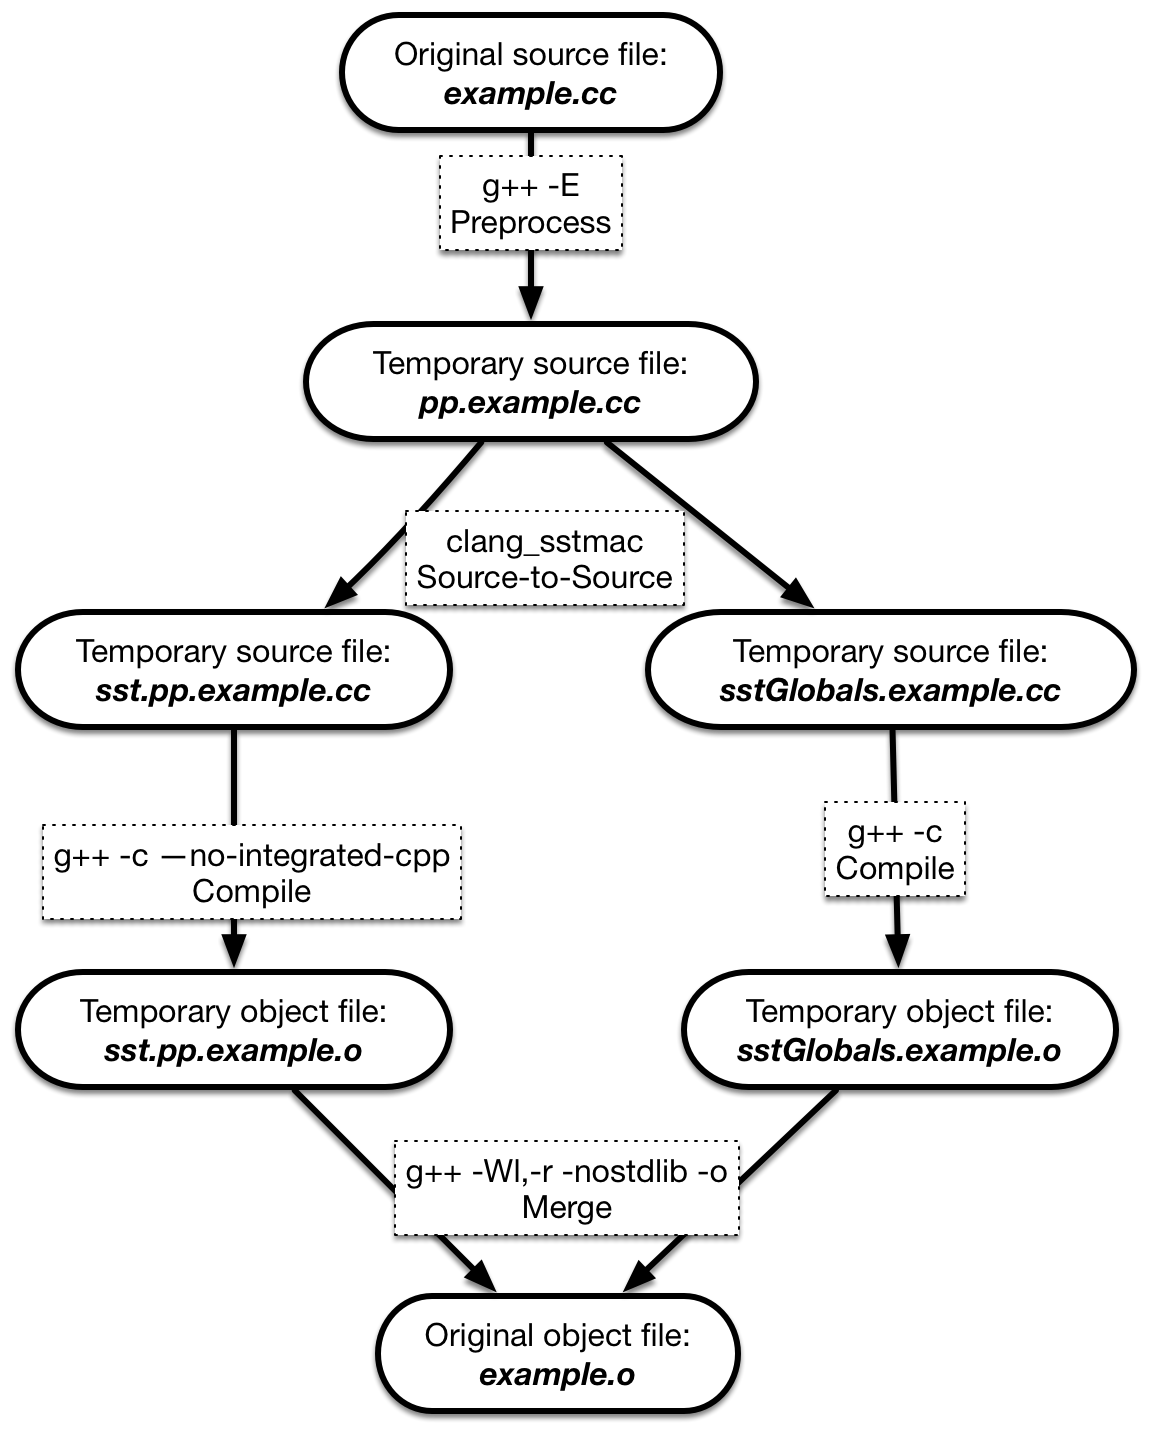
\includegraphics[width=0.66\textwidth]{figures/compilerWorkflow}
\caption{Source-to-source transformation workflow for SST compiler. For C source files, g++ can be swapped with gcc. The choice of underlying compiler is actually arbitrary and can be clang, gcc, icc, etc.}
\label{fig:compilerWorkflow}
\end{figure}

\subsection{Compiler workflow}
The source-to-source compiler operates on a pre-processed source file.
The source code transformation generates a temporary source file.
This temporary source file is then compiled into the target object file.
Global variables require static registration of C++ variables.
Here another temporary C++ source file (even if the original file is C)
is generated that has all static global variable registrations.
The corresponding object file is merged with the original object file,
creating a complete \sstmacro object file with the transformed code and C++ static registrations.
This workflow is shown in Figure \ref{fig:compilerWorkflow}.

\subsection{Compiler Environment Variables}

\subsubsection{SSTMAC\_SRC2SRC: Default 1}
If set to zero, deactivates the source-to-source transformation. 
The compiler wrapper will then compile the code into the simulator, but will not redirect any global variable accesses or perform any skeletonization.

\subsubsection{SSTMAC\_SKELETONIZE: Default 0}
If set to zero, deactivates skeletonization. 
This does not deactivate global variable redirection.
Thus, with \inlineshell{SSTMAC_SRC2SRC=1} and \inlineshell{SSTMAC_SKELETONIZE=0},
\sstmacro will act as an MPI emulator executing a full code but with global variables refactored to maintain correctness.

\subsubsection{SSTMAC\_MEMOIZE: Default 0}
If set to nonzero, activates memoization hooks. 
This deactivates all global variable refactoring, all symbol interception, and all skeletonization.

\subsubsection{SSTMAC\_HEADERS: No default}
The compiler wrapper will only redirect global variables that it knows should definitely be modified.
All global variables found in source files will be redirected.
\inlinecode{extern} global variables found in header files are more difficult.
Certain system global variables like \inlinecode{stderr} should not be modified and so are left as global variable constants.
By default, global variables in a header file are NOT redirected unless explicitly specified in a header configuration file.
The variable \inlineshell{SSTMAC_HEADERS} should give the full path of a file containing the list of header files.
Header file paths in the file should be one per line and should be the full path, not a relative path.

\subsubsection{SSTMAC\_DELETE\_TEMPS: Default 1}
If non-zero, the compiler cleans up all temporary files. 
If you wish to keep temporary files to view them for debugging, set to zero.
All temporary, intermediate source files will otherwise be deleted at the end of compilation.

\section{Basic Replacement Pragmas}
When skeletonization is active (see \inlineshell{SSTMAC_SKELETONIZE}), these pragmas will cause replacements in the original source code.
Pragmas appy to the next statement in the source code.
For compound statements such as a for-loop with a multi-statement body, the pragma applies to the entire for-loop.
\subsection{pragma sst delete: no arguments}
This deletes the next statement from the source code.
If the statement declares a variable that is used later in the code, this will cause a compile error.
Consider an example from the Lulesh source code.

\begin{CppCode}
#pragma sst delete
    testnorms_data.values[i] = normr/normr0;
\end{CppCode}
In the skeleton, the residual is not actually computed and the \inlinecode{testnorms_data} array is not actually allocated.
Thus this statement should be deleted and not actually executed in the skeleton.

\subsection{pragma sst replace [to\_replace:string] [new\_text:C++ expression]}
This applies a string replace to a variable or function call in the next statement.
Consider an example from Lulesh.

\begin{CppCode}
#pragma sst replace volo 1
   deltatime() = (Real_t(.5)*cbrt(volo(0)))/sqrt(Real_t(2.0)*einit);
\end{CppCode}
The function call \inlinecode{volo(0)} is not valid in the skeleton since volumes are not actually computed.
Here we simply estimate that all cells have unit volume replacing \inlinecode{volo(0)} with \inlinecode{1}.

\subsection{pragma sst init [new\_value:string]}
This pragma can only apply to a binary equals operator assigning a value.
The pragma changes the right-hand side to use the given new value.
For example, in Lulesh:

\begin{CppCode}
#pragma sst init nullptr
  destAddr = &domain.commDataSend[pmsg * maxPlaneComm] ;
\end{CppCode}
The send buffer \inlinecode{domain.commDataSend} is not allocated in the skeleton and thus is not valid to use.
The pragma causes the skeleton to simply set \inlinecode{destAddr} to \inlinecode{nullptr}.

\subsection{pragma sst return [new\_value:C++ expression]}
Pragma is equivalent to \inlinecode{pragma sst init}. This replaces the target of a return statement with the given expression.
This produces a compiler error if applied to anything but a return statement.

\subsection{pragma sst keep}
During the skeletonization process, some transformations occur automatically even without pragmas. 
For example, all MPI calls have input buffers converted to null pointers to indicate a simulated MPI call.
If the MPI call should be emulated with real payloads, the MPI call must be explicitly marked with \inlinecode{pragma keep}.
An example can be found in the HPCG skeleton:

\begin{CppCode}
#pragma sst keep
  MPI_Allreduce(&localNumberOfNonzeros, &totalNumberOfNonzeros, ...)
\end{CppCode}
The actual allreduce operation is carried out, summing the the local number into the total number of nonzeroes.

\subsection{pragma sst keep\_if [condition:C++ bool expression]}
More control over whether transformations are skipped is provided by \inlinecode{keep_if}.
An example is found in CoMD.

\begin{CppCode}
#pragma sst keep_if count < 16
   MPI_Allreduce(sendBuf, recvBuf, count, MPI_DOUBLE, MPI_SUM, MPI_COMM_WORLD);
\end{CppCode}
Any small allreduce operations are kept. 
Any allreduce operations larger than a given cutoff are simulated without emulating the actual buffer operations.

\subsection{pragma sst empty}
This pragma is applied to functions. The function prototype is kept, but an empty body is inserted instead of the actual code.
This can be useful for deleting large blocks of computation inside a function.

\subsection{pragma sst branch\_predict [condition:C++ expression]}
The branch prediction pragma can be applied in two different contexts.
We will revisit the pragma in the context of compute skeletonization below.
The branch prediction pragma should only be applied to an if-statement.
Much like the replace pragmas, it swaps out the given if condition with a new expression.

The branch prediction pragmas become necessary when skeletonizing.
Certain values may not be computed or certain variables marked null.
If these values are then used in an if predicate,
the skeletonizing compiler cannot deduce the correct behavior for the application.
When an ambiguous predicate is found, the compiler will usually print a warning and just assume the predicate is false.
Predicates are often almost always true or almost always false. 
Thus most uses of this pragma will simply supply \inlinecode{true} or \inlinecode{false} as the replacement.
However, any arbitrary C++ boolean expression can be given as the replacement.
The new predicate expression (like the original), must not involve any null variables.

\section{Memory Allocation Pragmas}
\subsection{pragma sst malloc}
Applied to any statement in which the right-hand side is a malloc. This sets the left-hand side to \inlinecode{NULL}.
This is critical for turning off large memory allocations on data structures not required for control-flow.


\subsection{pragma sst new}
Applied to any statement in which the right-hand side a C++ operator new. This sets the left-hand side to \inlinecode{nullptr}.
This is critical for turning off large memory allocations on data structures not required for control-flow.

\section{Data-Driven Type Pragmas}
\subsection{pragma sst null\_variable}
This applies to variable declarations. If pragma is not applied to a declaration, a compiler error is given.
A null variable is one in which all operations involving the variable should be deleted.
This usually applies to large data arrays that should never be allocated and therefore never dereferenced.
An example can be seen in CoMD:

\begin{CppCode}
#pragma sst null_variable
   int* nAtoms;         //!< total number of atoms in each box
\end{CppCode}
The array is not allocated and all statements operating on the array are deleted.

This pragma is much more powerful than simply using \inlinecode{pragma sst new}.
\inlinecode{pragma sst new} simply turns off a given memory allocation setting it to a null value.
If the array is dereferenced later in code, this causes a segmentation fault.
By marking a declaration as null, the compiler can flag where segmentation faults would occur when running the skeleton.

In most cases, all operations involving the null variable are deleted.
However, there may be cases where the compiler may decide deleting an operation cannot be done automatically since
it may affect control flow, e.g., if the variable is used inside an if-statement.
When this occurs, a compiler error is thrown flagging where the ambiguity occurs.
Another pragma must then be applied to that statement to tell the compiler how to proceed.

\subsection{pragma sst null\_type [type alias] [list allowed functions]}
This applies to C++ class variable declarations. If pragma is not applied to a declaration, a compiler error is given.
This essentially works the same way as \inlinecode{null_variable}, but allows certain member functions to be kept instead of deleted.
Consider an example from Lulesh:

\begin{CppCode}
#pragma sst null_type sstmac::vector size resize empty
   std::vector<Real_t> m_x ;  /* coordinates */
\end{CppCode} 
Here we wish to indicate the vector is ``null'' and should not actually allocate memory or allow array accesses.
However, we still wish to track the vector size and whether it is empty.
The first argument to the pragma is a new type name that implements the ``alias'' functionality.
For \inlinecode{std::vector}, \sstmacro automatically provides the alias.
For illustration, that code is reproduced here:

\begin{CppCode}
namespace sstmac {
class vector {
 public:
  void resize(unsigned long sz){
    size_ = sz;
  }

  unsigned long size() const {
    return size_;
  }

  template <class... Args>
  void push_back(Args... args){
    ++size_;
  }

  template <class... Args>
  void emplace_back(Args... args){
    ++size_;
  }

  bool empty() const {
    return size_ == 0;
  }

 private:
  unsigned long  size_;
};
}
\end{CppCode}
This empty vector class allows the type to track its size, but not actually hold any data.
All places in the Lulesh code that an \inlinecode{std::vector} is used are substituted with the new type.

The remaining arguments to the pragma are the list of functions we wish to mark as valid.
In this case, even though the alias vector class provides more functions, we only allow \inlinecode{size}, \inlinecode{resize}, and \inlinecode{empty} to be called.



\section{Compute Pragmas}
\subsection{pragma sst compute and pragma omp parallel}
Compute-intensive should not be executed natively.
Instead, a compute model should be used to estimate the elapsed time.
Compute model replacements are automatically triggered by any OpenMP parallel pragmas.
The corresponding block or for-loop is not executed, instead calling out to a compute model to estimate time.
Currently, compute modeling is done via a very basic static analysis.
The static analysis attempts to count the number of integer and floating point operations.
It also estimates the number of memory reads and writes.
These four counters are passed to a coarse-grained processor model for time estimates.
For more details, see \inlinecode{sstmac_compute_detailed} in the source code.
Numerous examples can be found in the Lulesh, HPCG, and CoMD skeleton applications.

\subsection{pragma sst loop\_count [integer: C++ expression]}
If the \inlinecode{sst compute} or \inlinecode{omp parallel} pragma are applied to an outer loop with one or more inner loops,
the compute model static analysis might fail.
This occurs when the inner loop control flow depends on the actual execution.
Any variables declared \emph{inside} the compute block are not valid to use in the compute estimate since they will be skeletonized and deleted.
Only variables in scope at the beginning of the outer loop are safe to use in compute modeling.

When the static analysis fails, a corresponding compiler error is thrown.
This usually requires giving a loop count hint.
Consider the example from HPCG:

\begin{CppCode}
#pragma omp parallel for
  for (local_int_t i=0; i< localNumberOfRows; i++) {
    int cur_nnz = nonzerosInRow[i];
   #pragma sst loop_count 27
    for (int j=0; j<cur_nnz; j++) mtxIndL[i][j] = mtxIndG[i][j];
  }
\end{CppCode}
The static analysis fails on \inlinecode{cur_nnz}.
However, that value is almost always 27.
Thus we can safely tell the compiler to just assume the loop count is 27.

\subsection{pragma sst branch\_predict [float: C++ expression]}
Similar to the way that loop counts can break the static analysis, if statements inside a loop skeletonized with \inlinecode{omp parallel} or \inlinecode{sst compute} can also be problematic.
If the predicate depends on a variable declared \emph{inside} the skeletonzied block,
the static analysis will break since it cannot predict when and how often to assume true or false.
In contrast to the branch prediction pragma previously used, branch prediction pragmas inside a compute block must give a number between 0 and 1.
This can either be a literal float or expression that computes a float value.
Consider an example from CoMD:

\begin{CppCode}
#pragma sst branch_predict 0.2
  if(r2 <= rCut2 && r2 > 0.0){
\end{CppCode}
Inside the compute block, a compute may or may not occur depending on whether a particle distance is less than a cutoff.
Based on the way CoMD constructs unit cells and halo regions, running CoMD shows that about 1 in 5 neighbor interactions are actually below the cutoff.
Thus we given the branch prediction the hint 0.2.

\subsection{pragma sst advance\_time [units] [time to advance by]}
This pragma advances the simulator time by the specified amounts of time. It can be placed before any statement. The units can be the following: sec, msec, usec or nsec for Seconds, milliseconds, microseconds and nanoseconds respectively. 

% !TEX root = manual.tex

\section{Memoization pragmas}\label{sec:memoization}

\subsection{Memoization models}
To understand the memoization pragmas, we first introduce how models get constructed in the SST/macro runtime.
Source-to-source transformations based on the pragmas causes the following hooks to get inserted:

\begin{CppCode}
int sstmac_startMemoize(const char* token, const char* model);
void sstmac_finish_memoize0(int tag, const char* token);
void sstmac_finish_memoize1(int tag, const char* token, double p1);
void sstmac_finish_memoize2(int tag, const char* token, double p1, double p2);
...
\end{CppCode}
A start call begins a memoization region for a specific name.
The start function must return an integer tag identifying the memoization instance.
This tag gets passed back into the finish function above.
This is primarily useful for thread-safe collection, but can be generally more useful.
The finish functions take input parameters. 
Given input parameters $x$,$y$ causes a function $F(x,y)$ to be fit to the timer or performance counters.

If building a skeleton application that uses memoization data, a different hook gets inserted:
\begin{CppCode}
void sstmac_compute_memoize0(const char* token);
void sstmac_compute_memoize1(const char* token, double p1);
void sstmac_compute_memoize2(const char* token, double p1, double p2);
...
\end{CppCode}
Assuming a model $F(x,y)$ has been fit in a memoization pass,
that function is invoked with the given parameters to estimate a time or performance counter.

Memoization models are implemented by inheriting from a standard class

\begin{CppCode}
struct RegressionModel {
...
virtual double compute(int n_params, const double params[], ImplicitState* state) = 0;
virtual int StartCollection() = 0;
virtual void finishCollection(int n_params, const double params[], ImplicitState* state) = 0;
...
\end{CppCode}
A call to \inlinecode{sstmac_finish_memoize2} causes \inlinecode{finishCollection(2,..)} to get invoked on the model.
The \inlinecode{states} object is discussed more later in \ref{subsec:implicitStates}.
For now, \inlinecode{compute} only returns a double (total time).
Generalized performance models are planned for future versions.
Models are registered using the SST/macro factory system. 
If wanting to add a least-squares model, factory register as:

\begin{CppCode}
struct least_squares : public regression model {
 FactoryRegister("least_squares", OperatingSystem::RegressionModel, least_squares)
\end{CppCode}

\subsection{pragma sst memoize [skeletonize(...)] [model(...)] [inputs(...)] [name(...)]}
\begin{itemize}
\item skeletonize: boolean for whether code block should still be executed or remove entirely (default: true)
\item model: string name for a type of model (e.g. linear, kmeans) specifying which model to construct and fit (no default)
\item inputs: a comma-separated list of C++ expressions that are the numeric inputs
\item name: a unique name to use for identifying the memoization region (default: see below)
\end{itemize}
If the \inlinecode{name} parameter is not given, the file and line number is used for basic expressions while the function name is used if applied to a function.
Consider the example:

\begin{CppCode}
#pragma sst memoize skeletonize(true) model(least_squares) inputs(ncol,nlink,nrow) 
void dgemm(int ncol, int nlink, int nrow, double* left, double* right);
\end{CppCode}
When running the memoization pass, the memoization hooks get invoked as:

\begin{CppCode}
int tag = sstmac_startMemoize("dgemm", "least_squares");
dgemm(....);
sstmac_finish_memoize3(tag, "dgemm", ncol, nlink, nrow);
\end{CppCode}
With \inlinecode{skeletonize} set to true, the skeleton app would be:

\begin{CppCode}
sstmac_computeMemoize("dgemm", ncol, nlink, nrow);
\end{CppCode}
With skeletonize set to false:

\begin{CppCode}
sstmac_computeMemoize("dgemm", ncol, nlink, nrow);
dgemm(...);
\end{CppCode}
Both the memoization function and the original function would both get invoked.

\subsection{pragma sst implicit\_state X(Y) ...}\label{subsec:implicitStates}
The implicit state pragma sets certain hardware or software states not captured by the inputs to the memoization pragma.
This might involve DVFS states, different runs of a task in which data is ``cold'' or ``hot'' in cache, or different types of cores.
The implicit state lasts for the scope of the statement:

\begin{CppCode}
#pragma sst implict_state ...
{
 //all statements here have that state
}

#pragma sst ImplicitState ...
fxn(...) //implicit state lasts the entire function
\end{CppCode}

The arguments to the pragma are best understood by example:

\begin{CppCode}
#pragma sst ImplicitState dvfs(1) cache(hot)
fxn(...)
\end{CppCode}
This causes a source code transformation to:

\begin{CppCode}
sstmac_set_ImplicitState2(dvfs,1,cache,hot);
fxn(...);
sstmac_unset_ImplicitState2(dvfs,cache);
\end{CppCode}
For now, the functions take integer arguments (this may get relaxed to arbitrary strings).
Thus, e.g. enums must be available or compilation will fail:

\begin{CppCode}
enum states {
 dvfs=0,
 cache=1
};
enum cache_states {
 cold=0,
 hot=1
};
\end{CppCode}

If a \inlinecode{sstmac_finish_memoize} function got invoked, the states could be read.
The class \inlinecode{ImplicitState} is a base class only and carries no data by default.
Specific memoization models are intended to be used only with known implicit state classes.
As such, the memoization model \inlinecode{collect}, etc, functions must dynamic cast to an expected type.
A library of standard implicit state implementations is planned for future releases.

%% !TEX root = manual.tex

\chapter{Issues and Limitations}
\section{Polling in applications}

Use of probe non-blocking functions in a loop, such as:


\begin{CppCode}
while(!flag){
 MPI_Iprobe( 0, 0, MPI_COMM_WORLD, &flag, &status );
}
\end{CppCode}
creates problems for the simulation. Virtual time never advances in the MPI\_Iprobe call. 
This causes an infinite loop that never returns to the discrete event manager. 
Even if configured so that time progresses, the code will work but will take a very long time to run.

\section{Fortran}
\label{subsec:issues:fortran}

\sstmacro previously provided some experimental support for Fortran90 applications. 
This has been discontinued for the foreseeable future.
For profiling existing apps written with Fortran, DUMPI traces can still be generated. 






%%% End document
\end{document}
